\documentclass[final]{beamer} 
\usetheme[headheight=10cm,footheight=5cm]{boxes}
\usetheme{toby}
\usepackage{booktabs}
\usepackage{etex}
\usepackage{amsmath,amssymb}
\usepackage[latin1]{inputenc}
\usepackage[english]{babel}
\usepackage{helvet}
\usepackage[T1]{fontenc}
\usepackage{textcomp}
\usepackage[orientation=landscape,size=a0,scale=1.4,debug]{beamerposter}   % e.g. for DIN-A0 poster
\usepackage{exscale}
\usepackage{pst-plot}
\usepackage{pstricks-add}
\usepackage{epsfig}
\usepackage{eulervm}
\usepackage{tikz}
\usepackage{array}
\usepackage{subfigure}
\usepackage{graphicx}
  
% \usepackage[size=custom,width=3.0,height=120,scale=2,debug]{beamerposter}  % e.g. custom size poster

\usepackage{beamerthemetoby}

\def\x{{\mathbf x}}
\def\z{{\mathbf z}}
\def\l{{\ell}}
\def\1{{\mathbf 1}}
\def\0{{\mathbf 0}}
\def\a{{\mathbf a}}
%\def\c{{\mathbf c}}
\def\p{{\mathbf p}}
\def\v{{\mathbf v}}
\def\n{{\mathbf n}}
\def\X{{\mathbf X}}
\def\Z{{\mathbf Z}}
\def\eg{e.g.}
\def\ZZ{{\mathcal Z}}
\def\hatx{{\mathbf {\hat x}}}
\def\hatf{{ \hat f}}
\def\hatw{{\bf \hat w}}
\def\hati{{\hat{\imath}}}
\def\tildej{\tilde{\jmath}}
\def\tildel{\tilde{\ell}}
\def\hatX{{\bf \hat X}}
\def\hatb{{\hat b}}
\def\ae{\text{~~a.e.}}
\def\as{\text{~~a.s.}}
\def\hatalpha{\mbox{\boldmath${\hat \alpha}$}}
\def\tildealpha{\mbox{\boldmath${\tilde \alpha}$}}
\def\tildebeta{\mbox{\boldmath${\tilde \beta}$}}
\def\hatDelta{\mbox{\boldmath${\hat \Delta}$}}
\def\Lambdab{{\boldsymbol\Lambda}}
\def\lambdab{{\boldsymbol\lambda}}
\def\kappab{{\boldsymbol\kappa}}
\def\rhob{{\boldsymbol\rho}}
\def\taub{{\boldsymbol\tau}}

\def\xib{{\boldsymbol\xi}}
\def\xibbar{\tilde{\boldsymbol{\xi}}}
\def\nub{{\boldsymbol\nu}}
\def\Gammab{{\boldsymbol\Gamma}}
\def\Thetab{{\boldsymbol\Theta}}
\def\Sigmab{{\boldsymbol\Sigma}}
\def\Deltab{{\boldsymbol\Delta}}
\def\betab{{\boldsymbol\beta}}
\def\epsilonb{{\boldsymbol\varepsilon}}
\def\varepsilonb{{\boldsymbol\varepsilon}}
\def\alphab{{\boldsymbol\alpha}}
\def\thetab{{\boldsymbol\theta}}
\def\gammab{{\boldsymbol\gamma}}
\def\alphabtilde{{\boldsymbol\tilde{\alpha}}}
\def\hatlambdab{{\boldsymbol{\hat\lambda}}}
\def\Gammab{{\boldsymbol\Gamma}}
\def\tildeGammab{{\bf \tilde{\boldsymbol\Gamma}}}
\def\y{{\mathbf y}}
\def\FFF{\text{F}}
\def\w{{\mathbf w}}
\def\vw{{\mathbf w}}
\def\D{{\mathbf D}}
\def\mX{{\mathbf D}}
\def\Y{{\mathbf Y}}
\def\YY{{\mathcal Y}}
\def\M{{\mathbf M}}
\def\B{{\mathbf B}}
\def\Q{{\mathbf Q}}
\def\C{{\mathbf C}}
\def\W{{\mathbf W}}
\def\d{{\mathbf d}}
\def\E{{\mathbb E}}
\def\PPP{{\mathbb E}}
\def\EE{{\mathbf E}}
\def\O{{O}}
\def\N{{\mathcal N}}
\def\o{{\mathcal o}}
\def\s{{\mathbf s}}
\def\CC{{\mathcal C}}
\def\VV{{\mathcal V}}
\def\NN{{\mathcal N}}
\def\KK{{\mathcal K}}
\def\CCC{{C}}
\def\L{{\mathcal L}}
\def\P{{\mathcal P}}
\def\PP{{\mathbf P}}
\def\PPP{{\mathbb P}}
\def\R{{\mathbf R}}
\def\RR{{\mathcal R}}
\def\S{{\mathcal S}}
\def\SS{{\mathbf SS}}
\def\H{{\mathcal H}}
\def\d{{\mathbf d}}
\def\e{{\mathbf e}}
\def\b{{\mathbf b}}
\def\cc{{\mathbf c}}
\def\u{{\mathbf u}}
\def\m{{\mathbf m}}
\def\hatD{{\bf \hat D}}
\def\tildeD{{\mathbf{\tilde{D}}}}
\def\tildeB{{\mathbf{\tilde{B}}}}
\def\tildeC{{\mathbf{\tilde{C}}}}
\def\tildex{{\mathbf{\tilde{x}}}}
\def\tildef{{ \tilde f}}
\def\hatE{{\bf \hat E}}
\def\hate{{\bf \hat e}}
\def\hatd{{\bf \hat d}}
\def\hatf{{ \hat f}}
\def\tilded{{\bf \tilde d}}
\def\Real{{\mathbb R}}
\def\r{{\mathbf r}}
\def\U{{\mathbf U}}
\def\UY{{\mathcal U}}
\def\u{{\mathbf u}}
\def\A{{\mathbf A}}
\def\G{{\mathbb G}}
\def\GG{{\mathcal G}}
\def\AA{{\mathcal A}}
\def\FF{{\mathcal F}}
\def\DD{{\mathcal D}}
\def\XX{{\mathcal X}}
\def\WW{{\mathcal W}}
\def\V{{\mathbf V}}
\def\K{{\mathbf K}}
\def\KK{{\mathcal K}}
\def\T{{\mathbf T}}
\def\TT{{\mathcal T}}
\def\I{{\mathbf I}}
\def\one{{\mathbb 1}}
\def\argmin{\operatornamewithlimits{arg\,min}}
\def\liminf{\operatornamewithlimits{lim\,inf}}
\def\argmax{\operatornamewithlimits{arg\,max}}
\def\Var{\operatorname{Var}}
\def\diag{\operatorname{diag}}
\def\trace{\operatorname{Tr}}
\def\range{\operatorname{range}}
\def\vec{\operatorname{vec}}
\def\sign{\operatorname{sign}}
\def\FL{\operatorname{FL}}
\def\corr{\operatorname{corr}}
\def\cov{\operatorname{cov}}
\def\st{~~\text{s.t.}~~}
\def\defin{\triangleq}
%\def\TODO{ {\color{red} TODO }}
\newcommand{\TODO}[1]{{\textbf{\color{red} TODO: #1}}}

\def\gi{ {\scriptscriptstyle \hspace*{-0.002cm}\mid\hspace*{-0.008cm}}  g}
\def\hi{  {\scriptscriptstyle \hspace*{-0.002cm}\mid\hspace*{-0.008cm}}  h}

%\renewcommand{\cite}{\citep}
\newcommand{\refEq}{\ref}
%\renewenvironment{displaymath}{\begin{equation}}{\end{equation}}
%\renewenvironment{multline*}{\begin{multline}}{\end{multline}}

%\renewcommand{\cite}{\citep}
% \newcommand{\citet}{\emcite}
% \renewenvironment{displaymath}{\begin{equation}}{\end{equation}}
%:w\renewenvironment{multline*}{\begin{multline}}{\end{multline}}

% \newtheorem{example}{Example} 
% 

%\newcommand{\InSet}[1]{\text{\textlbrackdbl} 1;#1 \text{\textrbrackdbl}}
\newcommand{\InSet}[1]{\llbracket 1;#1 \rrbracket}
\newcommand{\IntSet}[1]{\llbracket 1;#1 \rrbracket}
\renewcommand{\bf}{\textbf}

\newcommand{\Norm}[1]{\|#1\|}
\newcommand{\DualNorm}[1]{\|#1\|_{\ast}}
\newcommand{\NormUn}[1]{\|#1\|_1}
\newcommand{\NormDeux}[1]{\|#1\|_2}
\newcommand{\NormInf}[1]{\|#1\|_{\infty}}
\newcommand{\NormFro}[1]{\|#1\|_{\text{F}}}
\newcommand{\NormFrob}[1]{\|#1\|_{\text{F}}}

\newcommand{\INPUT}{ {\bfseries Input: }}

\newcommand{\rred}[1]{{\textcolor{red}{#1}}}
\definecolorset{rgb}{}{}{inriablue,0.35,0.31,0.75}
\newcommand{\bblue}[1]{{\textcolor{inriablue}{#1}}}

\title[]{\veryHuge{Clusterpath: an Algorithm for Clustering using Convex Fusion Penalties}}
\author[]{Toby Dylan Hocking \and
      Armand Joulin \and
      Francis Bach \and
      Jean-Philippe Vert}
    \institute[Sierra]{~}%DONT DELETE THIS
\begin{document}
\begin{frame}{} 
\begin{columns}[T]
\hfill
\begin{column}{0.315\paperwidth}
% \begin{block}{One minute overview}
% \begin{itemize}
% \item Solving large-scale \rred{structured sparse} regularized problems.
% \item Use of (accelerated) \rred{proximal gradient methods}.
% \item Proximal operator solved with \rred{network flow optimization}.
% \end{itemize}
% \end{block}
\begin{block}{The clustering problem: different appraoches}
\begin{minipage}{4in}
  Clustering: assign labels to $n$ points in $p$ dimensions
    $X\in\RR^{n\times p}$.
\end{minipage}
\hspace{1in}
\begin{minipage}{4in}
  Methods:
    \begin{itemize}
  \item K-means
  \item Hierarchical
  \item Mixture models
  \item Spectral (Ng \emph{et al.} 2001)
    \end{itemize}
\end{minipage}
\begin{minipage}{4in}
    Issues:
    \begin{itemize}
    \item Hierarchy
    \item Convexity
    \item Greediness
    \item Stability
    \item Interpretability 
  \end{itemize}
\end{minipage}
\end{block}


\begin{block}{Clusterpath: relaxing a hard fusion penalty}
\begin{itemize}
\item Hard-thresholding of differences is a combinatorial problem:
$
 \min_{    \alpha\in\RR^{n\times p}}       ||\alpha-X||_F^2 \text{  subject to  }
\sum_{i<j}1_{\alpha_i\neq\alpha_j} \leq t$
\item \alert{Relaxation:$\sum_{i<j}||\alpha_i-\alpha_j||_q w_{ij}\leq t$}
\item The Lagrange form is useful for optimization algorithms:
$$
\alpha^*(X,\lambda,q,w)=\operatorname{argmin}_{\alpha\in\RR^{n\times p}}
\frac 1 2||\alpha-X||_F^2+\lambda\sum_{i<j}||\alpha_i-\alpha_j||_q w_{ij}
$$ 
\item The \alert<1>{clusterpath} of $X$ is the path of optimal
  $\alpha^*$ obtained by varying $\lambda$, for fixed weights
  $w_{ij}\in\RR^+$ and norm $q\in\{1,2,\infty\}$.
\item 
 Related work: ``fused lasso'' Tibshirani and Saunders (2005),
``grouping pursuit'' Shen and Huang (2010), ``sum of norms'' Lindsten
\emph{et al.}  (2011).
\end{itemize} 
\end{block}
% Created by tikzDevice version 0.6.1 on 2011-06-27 01:00:50
% !TEX encoding = UTF-8 Unicode
\begin{tikzpicture}[x=1pt,y=1pt]
\definecolor[named]{drawColor}{rgb}{0.00,0.00,0.00}
\definecolor[named]{fillColor}{rgb}{1.00,1.00,1.00}
\fill[color=fillColor,] (0,0) rectangle (505.89,578.16);
\begin{scope}
\path[clip] (  0.00,  0.00) rectangle (505.89,578.16);
\end{scope}
\begin{scope}
\path[clip] (  0.00,  0.00) rectangle (505.89,578.16);
\end{scope}
\begin{scope}
\path[clip] (  0.00,  0.00) rectangle (505.89,578.16);
\end{scope}
\begin{scope}
\path[clip] (  0.00,  0.00) rectangle (505.89,578.16);
\end{scope}
\begin{scope}
\path[clip] (  0.00,  0.00) rectangle (505.89,578.16);
\end{scope}
\begin{scope}
\path[clip] (  0.00,  0.00) rectangle (505.89,578.16);
\end{scope}
\begin{scope}
\path[clip] (  0.00,  0.00) rectangle (505.89,578.16);
\end{scope}
\begin{scope}
\path[clip] (  0.00,  0.00) rectangle (505.89,578.16);
\end{scope}
\begin{scope}
\path[clip] (  0.00,  0.00) rectangle (505.89,578.16);
\end{scope}
\begin{scope}
\path[clip] (  0.00,  0.00) rectangle (505.89,578.16);
\end{scope}
\begin{scope}
\path[clip] (  0.00,  0.00) rectangle (505.89,578.16);
\end{scope}
\begin{scope}
\path[clip] (  0.00,  0.00) rectangle (505.89,578.16);

\draw[fill opacity=0.00,draw opacity=0.00,] (  0.00,  0.00) rectangle (505.89,578.16);
\end{scope}
\begin{scope}
\path[clip] (  0.00,  0.00) rectangle (505.89,578.16);
\definecolor[named]{drawColor}{rgb}{0.00,0.00,0.00}

\node[color=drawColor,anchor=base,inner sep=0pt, outer sep=0pt, scale=  0.60] at (247.62,537.46) {Norm and weights control the clusterpath%
};
\end{scope}
\begin{scope}
\path[clip] (  0.00,  0.00) rectangle (505.89,578.16);
\end{scope}
\begin{scope}
\path[clip] (  0.00,  0.00) rectangle (505.89,578.16);
\end{scope}
\begin{scope}
\path[clip] (  0.00,  0.00) rectangle (505.89,578.16);
\end{scope}
\begin{scope}
\path[clip] ( 32.71,478.66) rectangle ( 55.84,496.15);
\end{scope}
\begin{scope}
\path[clip] (  0.00,  0.00) rectangle (505.89,578.16);
\end{scope}
\begin{scope}
\path[clip] ( 32.71,478.66) rectangle ( 55.84,478.66);
\end{scope}
\begin{scope}
\path[clip] (  0.00,  0.00) rectangle (505.89,578.16);
\end{scope}
\begin{scope}
\path[clip] (  0.00,  0.00) rectangle (505.89,578.16);
\end{scope}
\begin{scope}
\path[clip] (  0.00,  0.00) rectangle (505.89,578.16);
\end{scope}
\begin{scope}
\path[clip] ( 32.71,280.67) rectangle ( 55.84,287.90);
\end{scope}
\begin{scope}
\path[clip] (  0.00,  0.00) rectangle (505.89,578.16);
\end{scope}
\begin{scope}
\path[clip] (  0.00,  0.00) rectangle (505.89,578.16);
\end{scope}
\begin{scope}
\path[clip] (  0.00,  0.00) rectangle (505.89,578.16);
\end{scope}
\begin{scope}
\path[clip] ( 32.71, 89.92) rectangle ( 55.84, 89.92);
\end{scope}
\begin{scope}
\path[clip] (  0.00,  0.00) rectangle (505.89,578.16);
\end{scope}
\begin{scope}
\path[clip] ( 32.71, 66.79) rectangle ( 55.84, 89.92);
\end{scope}
\begin{scope}
\path[clip] (  0.00,  0.00) rectangle (505.89,578.16);
\end{scope}
\begin{scope}
\path[clip] ( 32.71, 66.79) rectangle ( 55.84, 66.79);
\end{scope}
\begin{scope}
\path[clip] (  0.00,  0.00) rectangle (505.89,578.16);
\end{scope}
\begin{scope}
\path[clip] ( 55.84,478.66) rectangle ( 55.84,496.15);
\end{scope}
\begin{scope}
\path[clip] (  0.00,  0.00) rectangle (505.89,578.16);
\end{scope}
\begin{scope}
\path[clip] ( 55.84,478.66) rectangle ( 55.84,478.66);
\end{scope}
\begin{scope}
\path[clip] (  0.00,  0.00) rectangle (505.89,578.16);
\end{scope}
\begin{scope}
\path[clip] ( 55.84,287.90) rectangle ( 55.84,478.66);
\end{scope}
\begin{scope}
\path[clip] (  0.00,  0.00) rectangle (505.89,578.16);
\end{scope}
\begin{scope}
\path[clip] ( 55.84,280.67) rectangle ( 55.84,287.90);
\end{scope}
\begin{scope}
\path[clip] (  0.00,  0.00) rectangle (505.89,578.16);
\end{scope}
\begin{scope}
\path[clip] ( 55.84, 89.92) rectangle ( 55.84,280.67);
\end{scope}
\begin{scope}
\path[clip] (  0.00,  0.00) rectangle (505.89,578.16);
\end{scope}
\begin{scope}
\path[clip] ( 55.84, 89.92) rectangle ( 55.84, 89.92);
\end{scope}
\begin{scope}
\path[clip] (  0.00,  0.00) rectangle (505.89,578.16);
\end{scope}
\begin{scope}
\path[clip] ( 55.84, 66.79) rectangle ( 55.84, 89.92);
\end{scope}
\begin{scope}
\path[clip] (  0.00,  0.00) rectangle (505.89,578.16);
\end{scope}
\begin{scope}
\path[clip] ( 55.84, 66.79) rectangle ( 55.84, 66.79);
\end{scope}
\begin{scope}
\path[clip] (  0.00,  0.00) rectangle (505.89,578.16);
\end{scope}
\begin{scope}
\path[clip] ( 55.84,478.66) rectangle (180.75,496.15);
\end{scope}
\begin{scope}
\path[clip] (  0.00,  0.00) rectangle (505.89,578.16);
\end{scope}
\begin{scope}
\path[clip] ( 55.84,478.66) rectangle (180.75,478.66);
\end{scope}
\begin{scope}
\path[clip] (  0.00,  0.00) rectangle (505.89,578.16);
\end{scope}
\begin{scope}
\path[clip] ( 55.84,287.90) rectangle (180.75,478.66);
\end{scope}
\begin{scope}
\path[clip] (  0.00,  0.00) rectangle (505.89,578.16);
\end{scope}
\begin{scope}
\path[clip] ( 55.84,280.67) rectangle (180.75,287.90);
\end{scope}
\begin{scope}
\path[clip] (  0.00,  0.00) rectangle (505.89,578.16);
\end{scope}
\begin{scope}
\path[clip] ( 55.84, 89.92) rectangle (180.75,280.67);
\end{scope}
\begin{scope}
\path[clip] (  0.00,  0.00) rectangle (505.89,578.16);
\end{scope}
\begin{scope}
\path[clip] ( 55.84, 89.92) rectangle (180.75, 89.92);
\end{scope}
\begin{scope}
\path[clip] (  0.00,  0.00) rectangle (505.89,578.16);
\end{scope}
\begin{scope}
\path[clip] (  0.00,  0.00) rectangle (505.89,578.16);
\end{scope}
\begin{scope}
\path[clip] (  0.00,  0.00) rectangle (505.89,578.16);
\end{scope}
\begin{scope}
\path[clip] ( 55.84, 66.79) rectangle (180.75, 66.79);
\end{scope}
\begin{scope}
\path[clip] (  0.00,  0.00) rectangle (505.89,578.16);
\end{scope}
\begin{scope}
\path[clip] (180.75,478.66) rectangle (187.98,496.15);
\end{scope}
\begin{scope}
\path[clip] (  0.00,  0.00) rectangle (505.89,578.16);
\end{scope}
\begin{scope}
\path[clip] (180.75,478.66) rectangle (187.98,478.66);
\end{scope}
\begin{scope}
\path[clip] (  0.00,  0.00) rectangle (505.89,578.16);
\end{scope}
\begin{scope}
\path[clip] (180.75,287.90) rectangle (187.98,478.66);
\end{scope}
\begin{scope}
\path[clip] (  0.00,  0.00) rectangle (505.89,578.16);
\end{scope}
\begin{scope}
\path[clip] (180.75,280.67) rectangle (187.98,287.90);
\end{scope}
\begin{scope}
\path[clip] (  0.00,  0.00) rectangle (505.89,578.16);
\end{scope}
\begin{scope}
\path[clip] (180.75, 89.92) rectangle (187.98,280.67);
\end{scope}
\begin{scope}
\path[clip] (  0.00,  0.00) rectangle (505.89,578.16);
\end{scope}
\begin{scope}
\path[clip] (180.75, 89.92) rectangle (187.98, 89.92);
\end{scope}
\begin{scope}
\path[clip] (  0.00,  0.00) rectangle (505.89,578.16);
\end{scope}
\begin{scope}
\path[clip] (180.75, 66.79) rectangle (187.98, 89.92);
\end{scope}
\begin{scope}
\path[clip] (  0.00,  0.00) rectangle (505.89,578.16);
\end{scope}
\begin{scope}
\path[clip] (180.75, 66.79) rectangle (187.98, 66.79);
\end{scope}
\begin{scope}
\path[clip] (  0.00,  0.00) rectangle (505.89,578.16);
\end{scope}
\begin{scope}
\path[clip] (187.98,478.66) rectangle (312.89,496.15);
\end{scope}
\begin{scope}
\path[clip] (  0.00,  0.00) rectangle (505.89,578.16);
\end{scope}
\begin{scope}
\path[clip] (187.98,478.66) rectangle (312.89,478.66);
\end{scope}
\begin{scope}
\path[clip] (  0.00,  0.00) rectangle (505.89,578.16);
\end{scope}
\begin{scope}
\path[clip] (187.98,287.90) rectangle (312.89,478.66);
\end{scope}
\begin{scope}
\path[clip] (  0.00,  0.00) rectangle (505.89,578.16);
\end{scope}
\begin{scope}
\path[clip] (187.98,280.67) rectangle (312.89,287.90);
\end{scope}
\begin{scope}
\path[clip] (  0.00,  0.00) rectangle (505.89,578.16);
\end{scope}
\begin{scope}
\path[clip] (187.98, 89.92) rectangle (312.89,280.67);
\end{scope}
\begin{scope}
\path[clip] (  0.00,  0.00) rectangle (505.89,578.16);
\end{scope}
\begin{scope}
\path[clip] (187.98, 89.92) rectangle (312.89, 89.92);
\end{scope}
\begin{scope}
\path[clip] (  0.00,  0.00) rectangle (505.89,578.16);
\end{scope}
\begin{scope}
\path[clip] (  0.00,  0.00) rectangle (505.89,578.16);
\end{scope}
\begin{scope}
\path[clip] (  0.00,  0.00) rectangle (505.89,578.16);
\end{scope}
\begin{scope}
\path[clip] (187.98, 66.79) rectangle (312.89, 66.79);
\end{scope}
\begin{scope}
\path[clip] (  0.00,  0.00) rectangle (505.89,578.16);
\end{scope}
\begin{scope}
\path[clip] (312.89,478.66) rectangle (320.12,496.15);
\end{scope}
\begin{scope}
\path[clip] (  0.00,  0.00) rectangle (505.89,578.16);
\end{scope}
\begin{scope}
\path[clip] (312.89,478.66) rectangle (320.12,478.66);
\end{scope}
\begin{scope}
\path[clip] (  0.00,  0.00) rectangle (505.89,578.16);
\end{scope}
\begin{scope}
\path[clip] (312.89,287.90) rectangle (320.12,478.66);
\end{scope}
\begin{scope}
\path[clip] (  0.00,  0.00) rectangle (505.89,578.16);
\end{scope}
\begin{scope}
\path[clip] (312.89,280.67) rectangle (320.12,287.90);
\end{scope}
\begin{scope}
\path[clip] (  0.00,  0.00) rectangle (505.89,578.16);
\end{scope}
\begin{scope}
\path[clip] (312.89, 89.92) rectangle (320.12,280.67);
\end{scope}
\begin{scope}
\path[clip] (  0.00,  0.00) rectangle (505.89,578.16);
\end{scope}
\begin{scope}
\path[clip] (312.89, 89.92) rectangle (320.12, 89.92);
\end{scope}
\begin{scope}
\path[clip] (  0.00,  0.00) rectangle (505.89,578.16);
\end{scope}
\begin{scope}
\path[clip] (312.89, 66.79) rectangle (320.12, 89.92);
\end{scope}
\begin{scope}
\path[clip] (  0.00,  0.00) rectangle (505.89,578.16);
\end{scope}
\begin{scope}
\path[clip] (312.89, 66.79) rectangle (320.12, 66.79);
\end{scope}
\begin{scope}
\path[clip] (  0.00,  0.00) rectangle (505.89,578.16);
\end{scope}
\begin{scope}
\path[clip] (320.12,478.66) rectangle (445.03,496.15);
\end{scope}
\begin{scope}
\path[clip] (  0.00,  0.00) rectangle (505.89,578.16);
\end{scope}
\begin{scope}
\path[clip] (320.12,478.66) rectangle (445.03,478.66);
\end{scope}
\begin{scope}
\path[clip] (  0.00,  0.00) rectangle (505.89,578.16);
\end{scope}
\begin{scope}
\path[clip] (320.12,287.90) rectangle (445.03,478.66);
\end{scope}
\begin{scope}
\path[clip] (  0.00,  0.00) rectangle (505.89,578.16);
\end{scope}
\begin{scope}
\path[clip] (320.12,280.67) rectangle (445.03,287.90);
\end{scope}
\begin{scope}
\path[clip] (  0.00,  0.00) rectangle (505.89,578.16);
\end{scope}
\begin{scope}
\path[clip] (320.12, 89.92) rectangle (445.03,280.67);
\end{scope}
\begin{scope}
\path[clip] (  0.00,  0.00) rectangle (505.89,578.16);
\end{scope}
\begin{scope}
\path[clip] (320.12, 89.92) rectangle (445.03, 89.92);
\end{scope}
\begin{scope}
\path[clip] (  0.00,  0.00) rectangle (505.89,578.16);
\end{scope}
\begin{scope}
\path[clip] (  0.00,  0.00) rectangle (505.89,578.16);
\end{scope}
\begin{scope}
\path[clip] (  0.00,  0.00) rectangle (505.89,578.16);
\end{scope}
\begin{scope}
\path[clip] (320.12, 66.79) rectangle (445.03, 66.79);
\end{scope}
\begin{scope}
\path[clip] (  0.00,  0.00) rectangle (505.89,578.16);
\end{scope}
\begin{scope}
\path[clip] (445.03,478.66) rectangle (445.03,496.15);
\end{scope}
\begin{scope}
\path[clip] (  0.00,  0.00) rectangle (505.89,578.16);
\end{scope}
\begin{scope}
\path[clip] (445.03,478.66) rectangle (445.03,478.66);
\end{scope}
\begin{scope}
\path[clip] (  0.00,  0.00) rectangle (505.89,578.16);
\end{scope}
\begin{scope}
\path[clip] (445.03,287.90) rectangle (445.03,478.66);
\end{scope}
\begin{scope}
\path[clip] (  0.00,  0.00) rectangle (505.89,578.16);
\end{scope}
\begin{scope}
\path[clip] (445.03,280.67) rectangle (445.03,287.90);
\end{scope}
\begin{scope}
\path[clip] (  0.00,  0.00) rectangle (505.89,578.16);
\end{scope}
\begin{scope}
\path[clip] (445.03, 89.92) rectangle (445.03,280.67);
\end{scope}
\begin{scope}
\path[clip] (  0.00,  0.00) rectangle (505.89,578.16);
\end{scope}
\begin{scope}
\path[clip] (445.03, 89.92) rectangle (445.03, 89.92);
\end{scope}
\begin{scope}
\path[clip] (  0.00,  0.00) rectangle (505.89,578.16);
\end{scope}
\begin{scope}
\path[clip] (445.03, 66.79) rectangle (445.03, 89.92);
\end{scope}
\begin{scope}
\path[clip] (  0.00,  0.00) rectangle (505.89,578.16);
\end{scope}
\begin{scope}
\path[clip] (445.03, 66.79) rectangle (445.03, 66.79);
\end{scope}
\begin{scope}
\path[clip] (  0.00,  0.00) rectangle (505.89,578.16);
\end{scope}
\begin{scope}
\path[clip] (445.03,478.66) rectangle (462.53,496.15);
\end{scope}
\begin{scope}
\path[clip] (  0.00,  0.00) rectangle (505.89,578.16);
\end{scope}
\begin{scope}
\path[clip] (445.03,478.66) rectangle (462.53,478.66);
\end{scope}
\begin{scope}
\path[clip] (  0.00,  0.00) rectangle (505.89,578.16);
\end{scope}
\begin{scope}
\path[clip] (445.03,287.90) rectangle (462.53,478.66);
\end{scope}
\begin{scope}
\path[clip] (  0.00,  0.00) rectangle (505.89,578.16);
\end{scope}
\begin{scope}
\path[clip] (445.03,280.67) rectangle (462.53,287.90);
\end{scope}
\begin{scope}
\path[clip] (  0.00,  0.00) rectangle (505.89,578.16);
\end{scope}
\begin{scope}
\path[clip] (445.03, 89.92) rectangle (462.53,280.67);
\end{scope}
\begin{scope}
\path[clip] (  0.00,  0.00) rectangle (505.89,578.16);
\end{scope}
\begin{scope}
\path[clip] (445.03, 89.92) rectangle (462.53, 89.92);
\end{scope}
\begin{scope}
\path[clip] (  0.00,  0.00) rectangle (505.89,578.16);
\end{scope}
\begin{scope}
\path[clip] (445.03, 66.79) rectangle (462.53, 89.92);
\end{scope}
\begin{scope}
\path[clip] (  0.00,  0.00) rectangle (505.89,578.16);
\end{scope}
\begin{scope}
\path[clip] (445.03, 66.79) rectangle (462.53, 66.79);
\end{scope}
\begin{scope}
\path[clip] (  0.00,  0.00) rectangle (505.89,578.16);
\end{scope}
\begin{scope}
\path[clip] (462.53,478.66) rectangle (462.53,496.15);
\end{scope}
\begin{scope}
\path[clip] (  0.00,  0.00) rectangle (505.89,578.16);
\end{scope}
\begin{scope}
\path[clip] (462.53,478.66) rectangle (462.53,478.66);
\end{scope}
\begin{scope}
\path[clip] (  0.00,  0.00) rectangle (505.89,578.16);
\end{scope}
\begin{scope}
\path[clip] (462.53,287.90) rectangle (462.53,478.66);
\end{scope}
\begin{scope}
\path[clip] (  0.00,  0.00) rectangle (505.89,578.16);
\end{scope}
\begin{scope}
\path[clip] (462.53,280.67) rectangle (462.53,287.90);
\end{scope}
\begin{scope}
\path[clip] (  0.00,  0.00) rectangle (505.89,578.16);
\end{scope}
\begin{scope}
\path[clip] (462.53, 89.92) rectangle (462.53,280.67);
\end{scope}
\begin{scope}
\path[clip] (  0.00,  0.00) rectangle (505.89,578.16);
\end{scope}
\begin{scope}
\path[clip] (462.53, 89.92) rectangle (462.53, 89.92);
\end{scope}
\begin{scope}
\path[clip] (  0.00,  0.00) rectangle (505.89,578.16);
\end{scope}
\begin{scope}
\path[clip] (462.53, 66.79) rectangle (462.53, 89.92);
\end{scope}
\begin{scope}
\path[clip] (  0.00,  0.00) rectangle (505.89,578.16);
\end{scope}
\begin{scope}
\path[clip] (462.53, 66.79) rectangle (462.53, 66.79);
\end{scope}
\begin{scope}
\path[clip] (  0.00,  0.00) rectangle (505.89,578.16);
\end{scope}
\begin{scope}
\path[clip] ( 32.71,478.66) rectangle ( 55.84,496.15);
\end{scope}
\begin{scope}
\path[clip] (  0.00,  0.00) rectangle (505.89,578.16);
\end{scope}
\begin{scope}
\path[clip] ( 32.71,478.66) rectangle ( 55.84,478.66);
\end{scope}
\begin{scope}
\path[clip] (  0.00,  0.00) rectangle (505.89,578.16);
\end{scope}
\begin{scope}
\path[clip] (  0.00,  0.00) rectangle (505.89,578.16);
\end{scope}
\begin{scope}
\path[clip] (  0.00,  0.00) rectangle (505.89,578.16);
\end{scope}
\begin{scope}
\path[clip] (  0.00,  0.00) rectangle (505.89,578.16);
\end{scope}
\begin{scope}
\path[clip] (  0.00,  0.00) rectangle (505.89,578.16);
\end{scope}
\begin{scope}
\path[clip] (  0.00,  0.00) rectangle (505.89,578.16);
\end{scope}
\begin{scope}
\path[clip] ( 32.71,280.67) rectangle ( 55.84,287.90);
\end{scope}
\begin{scope}
\path[clip] (  0.00,  0.00) rectangle (505.89,578.16);
\end{scope}
\begin{scope}
\path[clip] (  0.00,  0.00) rectangle (505.89,578.16);
\end{scope}
\begin{scope}
\path[clip] (  0.00,  0.00) rectangle (505.89,578.16);
\end{scope}
\begin{scope}
\path[clip] (  0.00,  0.00) rectangle (505.89,578.16);
\end{scope}
\begin{scope}
\path[clip] (  0.00,  0.00) rectangle (505.89,578.16);
\end{scope}
\begin{scope}
\path[clip] (  0.00,  0.00) rectangle (505.89,578.16);
\end{scope}
\begin{scope}
\path[clip] ( 32.71, 89.92) rectangle ( 55.84, 89.92);
\end{scope}
\begin{scope}
\path[clip] (  0.00,  0.00) rectangle (505.89,578.16);
\end{scope}
\begin{scope}
\path[clip] ( 32.71, 66.79) rectangle ( 55.84, 89.92);
\end{scope}
\begin{scope}
\path[clip] (  0.00,  0.00) rectangle (505.89,578.16);
\end{scope}
\begin{scope}
\path[clip] ( 32.71, 66.79) rectangle ( 55.84, 66.79);
\end{scope}
\begin{scope}
\path[clip] (  0.00,  0.00) rectangle (505.89,578.16);
\end{scope}
\begin{scope}
\path[clip] ( 55.84,478.66) rectangle ( 55.84,496.15);
\end{scope}
\begin{scope}
\path[clip] (  0.00,  0.00) rectangle (505.89,578.16);
\end{scope}
\begin{scope}
\path[clip] ( 55.84,478.66) rectangle ( 55.84,478.66);
\end{scope}
\begin{scope}
\path[clip] (  0.00,  0.00) rectangle (505.89,578.16);
\end{scope}
\begin{scope}
\path[clip] ( 55.84,287.90) rectangle ( 55.84,478.66);
\end{scope}
\begin{scope}
\path[clip] (  0.00,  0.00) rectangle (505.89,578.16);
\end{scope}
\begin{scope}
\path[clip] ( 55.84,280.67) rectangle ( 55.84,287.90);
\end{scope}
\begin{scope}
\path[clip] (  0.00,  0.00) rectangle (505.89,578.16);
\end{scope}
\begin{scope}
\path[clip] ( 55.84, 89.92) rectangle ( 55.84,280.67);
\end{scope}
\begin{scope}
\path[clip] (  0.00,  0.00) rectangle (505.89,578.16);
\end{scope}
\begin{scope}
\path[clip] ( 55.84, 89.92) rectangle ( 55.84, 89.92);
\end{scope}
\begin{scope}
\path[clip] (  0.00,  0.00) rectangle (505.89,578.16);
\end{scope}
\begin{scope}
\path[clip] ( 55.84, 66.79) rectangle ( 55.84, 89.92);
\end{scope}
\begin{scope}
\path[clip] (  0.00,  0.00) rectangle (505.89,578.16);
\end{scope}
\begin{scope}
\path[clip] ( 55.84, 66.79) rectangle ( 55.84, 66.79);
\end{scope}
\begin{scope}
\path[clip] (  0.00,  0.00) rectangle (505.89,578.16);
\end{scope}
\begin{scope}
\path[clip] ( 55.84,478.66) rectangle (180.75,496.15);
\definecolor[named]{drawColor}{rgb}{0.50,0.50,0.50}
\definecolor[named]{fillColor}{rgb}{0.80,0.80,0.80}

\draw[color=drawColor,line width= 0.6pt,line cap=round,line join=round,fill=fillColor,] ( 55.84,478.66) rectangle (180.75,496.15);
\definecolor[named]{drawColor}{rgb}{0.00,0.00,0.00}

\node[color=drawColor,anchor=base,inner sep=0pt, outer sep=0pt, scale=  0.40] at (118.29,485.89) {$\textrm{norm}=1$%
};
\end{scope}
\begin{scope}
\path[clip] (  0.00,  0.00) rectangle (505.89,578.16);
\end{scope}
\begin{scope}
\path[clip] ( 55.84,478.66) rectangle (180.75,478.66);
\end{scope}
\begin{scope}
\path[clip] (  0.00,  0.00) rectangle (505.89,578.16);
\end{scope}
\begin{scope}
\path[clip] ( 55.84,287.90) rectangle (180.75,478.66);
\definecolor[named]{fillColor}{rgb}{1.00,1.00,1.00}

\draw[fill=fillColor,draw opacity=0.00,] ( 55.84,287.90) rectangle (180.75,478.66);
\definecolor[named]{drawColor}{rgb}{0.75,0.75,0.75}

\node[color=drawColor,anchor=base,inner sep=0pt, outer sep=0pt, scale=  0.59] at (121.10,387.01) {$\bar X$%
};
\definecolor[named]{drawColor}{rgb}{0.00,0.00,0.00}

\draw[color=drawColor,line width= 1.1pt,line join=round,fill opacity=0.00,] (121.10,389.26) --
	(121.10,386.99) --
	(121.10,384.78) --
	(121.10,383.89) --
	(121.10,383.08) --
	(121.10,382.27) --
	(121.10,381.46) --
	(121.10,380.65) --
	(121.10,379.84) --
	(121.10,379.03) --
	(121.10,378.22) --
	(121.10,377.41) --
	(121.10,376.67) --
	(121.63,376.18) --
	(122.57,375.80) --
	(123.52,375.42) --
	(124.47,375.04) --
	(125.41,374.66) --
	(126.36,374.29) --
	(127.22,373.91) --
	(127.96,373.54) --
	(128.69,373.18) --
	(129.42,372.81) --
	(130.14,372.45) --
	(130.70,372.09) --
	(131.23,371.73) --
	(131.77,371.37) --
	(132.30,371.02) --
	(132.83,370.66) --
	(133.36,370.35) --
	(133.89,370.14) --
	(134.42,369.96) --
	(134.95,369.79) --
	(135.48,369.61) --
	(136.13,369.44) --
	(136.83,369.26) --
	(137.52,369.09) --
	(138.22,368.91) --
	(138.91,368.74) --
	(139.47,368.57) --
	(140.00,368.39) --
	(140.52,368.22) --
	(141.03,368.05) --
	(141.55,367.87) --
	(142.07,367.70) --
	(142.59,367.53) --
	(143.11,367.36) --
	(143.62,367.18) --
	(144.14,367.01) --
	(144.65,366.84);

\draw[color=drawColor,line width= 1.1pt,line join=round,fill opacity=0.00,] (121.10,389.26) --
	(121.10,386.99) --
	(121.10,384.71) --
	(121.10,381.91) --
	(121.10,379.07) --
	(121.10,376.24) --
	(121.10,373.41) --
	(121.10,370.58) --
	(121.10,367.74) --
	(121.10,364.91) --
	(121.10,362.08) --
	(121.10,359.25) --
	(121.10,356.74) --
	(121.12,355.26) --
	(120.56,354.12) --
	(119.99,352.98) --
	(119.42,351.85) --
	(118.85,350.71) --
	(118.28,349.57) --
	(117.72,348.45) --
	(117.17,347.35) --
	(116.62,346.25) --
	(116.07,345.15) --
	(115.52,344.05) --
	(114.98,342.98) --
	(114.45,341.91) --
	(113.92,340.84) --
	(113.38,339.77) --
	(112.91,338.71) --
	(112.55,337.65) --
	(112.20,336.59) --
	(111.85,335.54) --
	(111.50,334.48) --
	(111.14,333.42) --
	(110.80,332.38) --
	(110.45,331.33) --
	(110.10,330.29) --
	(109.75,329.24) --
	(109.40,328.19) --
	(109.05,327.15) --
	(108.74,326.11) --
	(108.56,325.07) --
	(108.39,324.03) --
	(108.21,323.00) --
	(108.04,321.96) --
	(107.87,320.93) --
	(107.70,319.89) --
	(107.52,318.98) --
	(107.35,318.12) --
	(107.18,317.27);

\draw[color=drawColor,line width= 1.1pt,line join=round,fill opacity=0.00,] (121.10,389.26) --
	(121.10,386.99) --
	(121.10,384.78) --
	(121.10,383.89) --
	(121.10,383.08) --
	(121.10,382.27) --
	(121.10,381.46) --
	(121.10,380.65) --
	(121.10,379.84) --
	(121.10,379.03) --
	(121.10,378.22) --
	(121.10,377.41) --
	(121.10,376.67) --
	(121.12,376.18) --
	(120.56,375.80) --
	(119.99,375.42) --
	(119.42,375.04) --
	(118.85,374.66) --
	(118.28,374.29) --
	(117.72,373.91) --
	(117.17,373.54) --
	(116.62,373.18) --
	(116.07,372.81) --
	(115.52,372.45) --
	(114.98,372.09) --
	(114.45,371.73) --
	(113.92,371.37) --
	(113.38,371.02) --
	(112.73,370.66) --
	(111.85,370.27) --
	(110.97,369.78) --
	(110.09,369.25) --
	(109.21,368.72) --
	(108.34,368.19) --
	(107.46,367.67) --
	(106.59,367.15) --
	(105.72,366.62) --
	(104.85,366.10) --
	(103.98,365.58) --
	(103.11,365.06) --
	(102.24,364.54) --
	(101.37,364.02) --
	(100.51,363.50) --
	( 99.65,362.98) --
	( 98.78,362.46) --
	( 97.92,361.94) --
	( 97.06,361.43) --
	( 96.19,360.91) --
	( 95.34,360.39) --
	( 94.48,359.88);

\draw[color=drawColor,line width= 1.1pt,line join=round,fill opacity=0.00,] (121.10,389.26) --
	(121.10,386.99) --
	(121.10,384.71) --
	(121.10,381.91) --
	(121.10,379.07) --
	(121.10,376.24) --
	(121.10,373.41) --
	(121.10,370.58) --
	(121.10,367.74) --
	(121.10,364.91) --
	(121.10,362.08) --
	(121.10,359.25) --
	(121.10,356.48) --
	(121.63,354.26) --
	(122.57,352.56) --
	(123.52,350.85) --
	(124.47,349.15) --
	(125.42,347.44) --
	(126.37,345.74) --
	(127.60,344.06) --
	(129.24,342.41) --
	(130.89,340.76) --
	(132.54,339.11) --
	(134.19,337.46) --
	(135.80,335.85) --
	(137.40,334.24) --
	(139.00,332.64) --
	(140.61,331.04) --
	(142.21,329.44) --
	(143.79,327.85) --
	(145.38,326.27) --
	(146.96,324.68) --
	(148.54,323.10) --
	(150.13,321.52) --
	(151.70,319.95) --
	(153.27,318.38) --
	(154.84,316.81) --
	(156.41,315.24) --
	(157.97,313.67) --
	(159.54,312.11) --
	(161.10,310.54) --
	(162.66,308.99) --
	(164.21,307.43) --
	(165.77,305.88) --
	(167.32,304.32) --
	(168.88,302.77) --
	(170.43,301.21) --
	(171.98,299.66) --
	(173.53,298.12) --
	(175.07,296.58);

\draw[color=drawColor,line width= 1.1pt,line join=round,fill opacity=0.00,] (121.10,389.26) --
	(121.10,386.99) --
	(121.10,384.71) --
	(121.10,381.91) --
	(121.10,379.07) --
	(121.10,376.24) --
	(121.10,373.41) --
	(121.10,370.58) --
	(121.10,367.74) --
	(121.10,364.91) --
	(121.10,362.08) --
	(121.10,359.25) --
	(121.10,356.74) --
	(121.63,355.26) --
	(122.57,354.12) --
	(123.52,352.98) --
	(124.47,351.85) --
	(125.41,350.71) --
	(126.36,349.57) --
	(127.22,348.45) --
	(127.96,347.35) --
	(128.69,346.25) --
	(129.42,345.15) --
	(130.14,344.05) --
	(130.70,342.98) --
	(131.23,341.91) --
	(131.77,340.84) --
	(132.30,339.77) --
	(132.83,338.71) --
	(133.36,337.65) --
	(133.89,336.59) --
	(134.42,335.54) --
	(134.94,334.48) --
	(135.47,333.42) --
	(135.73,332.38) --
	(135.90,331.33) --
	(136.08,330.29) --
	(136.25,329.24) --
	(136.43,328.19) --
	(136.60,327.15) --
	(136.78,326.11) --
	(136.95,325.07) --
	(137.12,324.03) --
	(137.29,323.00) --
	(137.47,321.96) --
	(137.64,320.93) --
	(137.81,319.89) --
	(137.98,318.73) --
	(138.16,317.53) --
	(138.33,316.33);

\draw[color=drawColor,line width= 1.1pt,line join=round,fill opacity=0.00,] (121.10,389.26) --
	(121.10,391.52) --
	(121.10,393.78) --
	(121.10,395.82) --
	(121.10,397.84) --
	(121.10,399.86) --
	(121.10,401.89) --
	(121.10,403.91) --
	(121.10,405.93) --
	(121.10,407.96) --
	(121.10,409.98) --
	(121.10,412.00) --
	(121.10,412.96) --
	(120.33,413.46) --
	(119.00,413.83) --
	(117.68,414.21) --
	(116.35,414.59) --
	(115.02,414.97) --
	(113.70,415.35) --
	(112.39,415.72) --
	(111.11,416.09) --
	(109.82,416.46) --
	(108.54,416.82) --
	(107.26,417.19) --
	(106.00,417.55) --
	(104.76,417.91) --
	(103.51,418.26) --
	(102.26,418.62) --
	(101.02,418.97) --
	( 99.79,419.33) --
	( 98.55,419.68) --
	( 97.32,420.03) --
	( 96.09,420.38) --
	( 94.86,420.73) --
	( 93.64,421.08) --
	( 92.42,421.43) --
	( 91.20,421.78) --
	( 89.98,422.13) --
	( 88.76,422.48) --
	( 87.54,422.82) --
	( 86.32,423.17) --
	( 85.11,423.52) --
	( 83.90,423.86) --
	( 82.69,424.21) --
	( 81.49,424.55) --
	( 80.28,424.90) --
	( 79.07,425.24) --
	( 77.86,425.59) --
	( 76.66,426.04) --
	( 75.46,426.55);

\draw[color=drawColor,line width= 1.1pt,line join=round,fill opacity=0.00,] (121.10,389.26) --
	(121.10,391.52) --
	(121.10,393.78) --
	(121.10,395.82) --
	(121.10,397.84) --
	(121.10,399.86) --
	(121.10,401.89) --
	(121.10,403.91) --
	(121.10,405.93) --
	(121.10,407.96) --
	(121.10,409.98) --
	(121.10,412.00) --
	(121.10,414.45) --
	(121.63,416.18) --
	(122.57,417.50) --
	(123.52,418.83) --
	(124.47,420.16) --
	(125.41,421.48) --
	(126.36,422.81) --
	(127.22,424.12) --
	(127.96,425.40) --
	(128.69,426.68) --
	(129.42,427.97) --
	(130.20,429.25) --
	(131.40,430.40) --
	(132.64,431.47) --
	(133.89,432.53) --
	(135.14,433.60) --
	(136.38,434.67) --
	(137.61,435.73) --
	(138.85,436.78) --
	(140.08,437.84) --
	(141.31,438.89) --
	(142.54,439.95) --
	(143.76,441.00) --
	(144.98,442.04) --
	(146.20,443.09) --
	(147.42,444.14) --
	(148.64,445.18) --
	(149.86,446.22) --
	(151.08,447.27) --
	(152.29,448.23) --
	(153.50,449.10) --
	(154.71,449.96) --
	(155.91,450.82) --
	(157.12,451.69) --
	(158.33,452.55) --
	(159.54,453.41) --
	(160.74,454.27) --
	(161.94,455.13);

\draw[color=drawColor,line width= 1.1pt,line join=round,fill opacity=0.00,] (121.10,389.26) --
	(121.10,391.52) --
	(121.10,393.78) --
	(121.10,395.82) --
	(121.10,397.84) --
	(121.10,399.86) --
	(121.10,401.89) --
	(121.10,403.91) --
	(121.10,405.93) --
	(121.10,407.96) --
	(121.10,409.98) --
	(121.10,412.00) --
	(121.10,414.45) --
	(119.21,416.18) --
	(117.50,417.50) --
	(115.80,418.83) --
	(114.09,420.16) --
	(112.39,421.48) --
	(110.68,422.81) --
	(109.00,424.12) --
	(107.35,425.40) --
	(105.70,426.68) --
	(104.05,427.97) --
	(102.40,429.25) --
	(100.79,430.71) --
	( 99.18,432.32) --
	( 97.58,433.92) --
	( 95.98,435.52) --
	( 94.38,437.12) --
	( 92.79,438.71) --
	( 91.21,440.29) --
	( 89.63,441.88) --
	( 88.04,443.46) --
	( 86.46,445.04) --
	( 84.89,446.61) --
	( 83.32,448.18) --
	( 81.75,449.75) --
	( 80.18,451.32) --
	( 78.61,452.89) --
	( 77.05,454.45) --
	( 75.48,456.02) --
	( 73.93,457.57) --
	( 72.37,459.13) --
	( 70.82,460.68) --
	( 69.26,462.24) --
	( 67.71,463.79) --
	( 66.16,465.35) --
	( 64.61,466.90) --
	( 63.06,468.44) --
	( 61.52,469.98);

\draw[color=drawColor,line width= 1.1pt,line join=round,fill opacity=0.00,] (121.10,389.26) --
	(121.10,391.52) --
	(121.10,393.78) --
	(121.10,395.82) --
	(121.10,397.84) --
	(121.10,399.86) --
	(121.10,401.89) --
	(121.10,403.91) --
	(121.10,405.93) --
	(121.10,407.96) --
	(121.10,409.98) --
	(121.10,412.00) --
	(121.10,414.45) --
	(121.12,416.18) --
	(120.56,417.50) --
	(119.99,418.83) --
	(119.42,420.16) --
	(118.85,421.48) --
	(118.28,422.81) --
	(117.72,424.12) --
	(117.17,425.40) --
	(116.62,426.68) --
	(116.07,427.97) --
	(115.52,429.25) --
	(114.98,430.40) --
	(114.45,431.47) --
	(113.92,432.53) --
	(113.38,433.60) --
	(112.91,434.67) --
	(112.55,435.73) --
	(112.20,436.78) --
	(111.85,437.84) --
	(111.50,438.89) --
	(111.14,439.95) --
	(110.80,441.00) --
	(110.45,442.04) --
	(110.10,443.09) --
	(109.75,444.14) --
	(109.40,445.18) --
	(109.05,446.22) --
	(108.68,447.27) --
	(108.16,448.38) --
	(107.64,449.58) --
	(107.12,450.79) --
	(106.61,452.00) --
	(106.09,453.21) --
	(105.57,454.42) --
	(105.05,455.63) --
	(104.54,456.83) --
	(104.02,458.03);

\draw[color=drawColor,line width= 1.1pt,line join=round,fill opacity=0.00,] (121.10,389.26) --
	(121.10,391.52) --
	(121.10,393.78) --
	(121.10,395.82) --
	(121.10,397.84) --
	(121.10,399.86) --
	(121.10,401.89) --
	(121.10,403.91) --
	(121.10,405.93) --
	(121.10,407.96) --
	(121.10,409.98) --
	(121.10,412.00) --
	(121.10,412.96) --
	(121.63,413.46) --
	(122.57,413.83) --
	(123.52,414.21) --
	(124.47,414.59) --
	(125.41,414.97) --
	(126.36,415.35) --
	(127.22,415.72) --
	(127.96,416.09) --
	(128.69,416.46) --
	(129.42,416.82) --
	(130.14,417.19) --
	(130.70,417.55) --
	(131.23,417.91) --
	(131.77,418.26) --
	(132.30,418.62) --
	(132.83,418.97) --
	(133.36,419.33) --
	(133.89,419.68) --
	(134.42,420.03) --
	(134.95,420.38) --
	(135.48,420.73) --
	(136.13,421.08) --
	(136.83,421.43) --
	(137.52,421.78) --
	(138.22,422.13) --
	(138.92,422.48) --
	(139.75,422.82) --
	(140.62,423.17) --
	(141.49,423.52) --
	(142.35,423.86) --
	(143.21,424.21) --
	(144.08,424.55) --
	(144.94,424.90) --
	(145.80,425.24) --
	(146.67,425.59) --
	(147.52,425.83) --
	(148.38,426.00);

\draw[color=drawColor,line cap=round,line join=round,fill=fillColor,] (144.65,366.84) circle (  2.13);

\draw[color=drawColor,line cap=round,line join=round,fill=fillColor,] (107.18,317.27) circle (  2.13);

\draw[color=drawColor,line cap=round,line join=round,fill=fillColor,] ( 94.48,359.88) circle (  2.13);

\draw[color=drawColor,line cap=round,line join=round,fill=fillColor,] (175.07,296.57) circle (  2.13);

\draw[color=drawColor,line cap=round,line join=round,fill=fillColor,] (138.33,316.32) circle (  2.13);

\draw[color=drawColor,line cap=round,line join=round,fill=fillColor,] ( 75.46,426.55) circle (  2.13);

\draw[color=drawColor,line cap=round,line join=round,fill=fillColor,] (161.94,455.13) circle (  2.13);

\draw[color=drawColor,line cap=round,line join=round,fill=fillColor,] ( 61.51,469.99) circle (  2.13);

\draw[color=drawColor,line cap=round,line join=round,fill=fillColor,] (104.02,458.03) circle (  2.13);

\draw[color=drawColor,line cap=round,line join=round,fill=fillColor,] (148.38,426.00) circle (  2.13);
\definecolor[named]{drawColor}{rgb}{0.50,0.50,0.50}

\draw[color=drawColor,line width= 0.6pt,line cap=round,line join=round,fill opacity=0.00,] ( 55.84,287.90) rectangle (180.75,478.66);
\end{scope}
\begin{scope}
\path[clip] (  0.00,  0.00) rectangle (505.89,578.16);
\end{scope}
\begin{scope}
\path[clip] ( 55.84,280.67) rectangle (180.75,287.90);
\end{scope}
\begin{scope}
\path[clip] (  0.00,  0.00) rectangle (505.89,578.16);
\end{scope}
\begin{scope}
\path[clip] ( 55.84, 89.92) rectangle (180.75,280.67);
\definecolor[named]{fillColor}{rgb}{1.00,1.00,1.00}

\draw[fill=fillColor,draw opacity=0.00,] ( 55.84, 89.92) rectangle (180.75,280.67);
\definecolor[named]{drawColor}{rgb}{0.75,0.75,0.75}

\node[color=drawColor,anchor=base,inner sep=0pt, outer sep=0pt, scale=  0.59] at (121.10,189.03) {$\bar X$%
};
\definecolor[named]{drawColor}{rgb}{0.00,0.00,0.00}

\draw[color=drawColor,line width= 1.1pt,line join=round,fill opacity=0.00,] (121.10,191.27) --
	(121.10,187.15) --
	(121.10,183.03) --
	(121.10,178.91) --
	(121.10,174.78) --
	(121.10,170.66) --
	(121.10,166.54) --
	(121.10,162.41) --
	(121.10,158.29) --
	(121.10,154.17) --
	(121.68,151.31) --
	(122.92,150.12) --
	(123.82,150.99) --
	(124.73,151.87) --
	(125.47,152.71) --
	(125.88,153.45) --
	(126.29,154.20) --
	(126.71,154.94) --
	(127.11,155.68) --
	(127.48,156.33) --
	(127.82,156.95) --
	(128.71,157.35) --
	(129.64,157.73) --
	(130.57,158.11) --
	(131.46,158.47) --
	(132.27,158.81) --
	(132.99,159.10) --
	(133.72,159.40) --
	(134.40,159.69) --
	(134.86,159.97) --
	(135.27,160.25) --
	(135.61,160.53) --
	(135.95,160.81) --
	(136.29,161.09) --
	(136.63,161.37) --
	(136.97,161.65) --
	(137.30,161.93) --
	(137.64,162.21) --
	(137.98,162.49) --
	(138.32,162.77) --
	(138.67,163.12) --
	(139.38,163.80) --
	(140.10,164.49) --
	(140.76,165.13) --
	(141.41,165.75) --
	(142.07,166.38) --
	(142.72,167.00) --
	(143.37,167.63) --
	(144.02,168.25) --
	(144.65,168.85);

\draw[color=drawColor,line width= 1.1pt,line join=round,fill opacity=0.00,] (121.10,191.27) --
	(121.10,187.15) --
	(121.10,183.03) --
	(121.10,178.91) --
	(121.10,174.78) --
	(121.10,170.66) --
	(121.10,166.54) --
	(121.10,162.41) --
	(121.10,158.29) --
	(121.10,154.17) --
	(121.68,151.31) --
	(122.92,149.92) --
	(123.82,147.73) --
	(124.73,145.55) --
	(125.47,143.48) --
	(125.88,141.63) --
	(126.29,139.79) --
	(126.71,137.94) --
	(127.11,136.21) --
	(127.48,135.04) --
	(127.81,133.93) --
	(126.81,133.21) --
	(125.87,132.53) --
	(124.94,131.84) --
	(124.06,131.19) --
	(123.24,130.59) --
	(122.52,130.06) --
	(121.79,129.53) --
	(121.08,129.01) --
	(120.39,128.50) --
	(119.70,128.00) --
	(119.02,127.50) --
	(118.34,127.00) --
	(117.66,126.50) --
	(116.97,126.00) --
	(116.29,125.50) --
	(115.61,125.00) --
	(114.93,124.49) --
	(114.24,123.99) --
	(113.56,123.49) --
	(112.88,122.99) --
	(112.20,122.50) --
	(111.52,121.99) --
	(110.88,121.53) --
	(110.26,121.07) --
	(109.64,120.62) --
	(109.02,120.16) --
	(108.40,119.71) --
	(107.78,119.33) --
	(107.18,119.28);

\draw[color=drawColor,line width= 1.1pt,line join=round,fill opacity=0.00,] (121.10,191.27) --
	(121.10,187.15) --
	(121.10,183.03) --
	(121.10,178.91) --
	(121.10,174.78) --
	(121.10,170.66) --
	(121.10,166.54) --
	(121.10,162.41) --
	(121.10,158.29) --
	(121.10,154.17) --
	(121.68,151.31) --
	(122.92,150.12) --
	(123.82,150.99) --
	(124.73,151.87) --
	(125.47,152.71) --
	(125.88,153.45) --
	(126.29,154.20) --
	(126.71,154.94) --
	(127.11,155.68) --
	(127.48,156.33) --
	(127.81,156.95) --
	(126.61,157.35) --
	(125.09,157.73) --
	(123.56,158.11) --
	(122.11,158.47) --
	(120.77,158.81) --
	(119.59,159.10) --
	(118.41,159.40) --
	(117.23,159.69) --
	(116.11,159.97) --
	(114.99,160.25) --
	(113.87,160.53) --
	(112.75,160.81) --
	(111.63,161.09) --
	(110.51,161.37) --
	(109.40,161.65) --
	(108.28,161.93) --
	(107.16,162.21) --
	(106.04,162.49) --
	(104.92,162.77) --
	(103.81,162.97) --
	(103.18,162.84) --
	(102.64,162.71) --
	(101.53,162.59) --
	(100.35,162.48) --
	( 99.16,162.36) --
	( 97.98,162.24) --
	( 96.80,162.12) --
	( 95.62,162.01) --
	( 94.48,161.90);

\draw[color=drawColor,line width= 1.1pt,line join=round,fill opacity=0.00,] (121.10,191.27) --
	(121.10,187.15) --
	(121.10,183.03) --
	(121.10,178.91) --
	(121.10,174.78) --
	(121.10,170.66) --
	(121.10,166.54) --
	(121.10,162.41) --
	(121.10,158.29) --
	(121.10,154.17) --
	(121.68,151.31) --
	(122.92,149.92) --
	(123.82,147.73) --
	(124.73,145.55) --
	(126.29,143.48) --
	(129.16,141.63) --
	(132.03,139.79) --
	(134.89,137.94) --
	(137.72,135.94) --
	(140.24,133.42) --
	(142.61,131.05) --
	(144.16,129.50) --
	(145.63,128.03) --
	(147.09,126.57) --
	(148.49,125.17) --
	(149.78,123.88) --
	(150.92,122.74) --
	(152.05,121.61) --
	(153.18,120.48) --
	(154.27,119.40) --
	(155.34,118.32) --
	(156.42,117.24) --
	(157.50,116.17) --
	(158.57,115.09) --
	(159.65,114.02) --
	(160.72,112.94) --
	(161.80,111.86) --
	(162.87,110.79) --
	(163.95,109.71) --
	(165.02,108.64) --
	(166.09,107.57) --
	(167.16,106.50) --
	(168.24,105.42) --
	(169.24,104.42) --
	(170.22,103.45) --
	(171.20,102.47) --
	(172.17,101.49) --
	(173.15,100.51) --
	(174.12, 99.54) --
	(175.07, 98.59);

\draw[color=drawColor,line width= 1.1pt,line join=round,fill opacity=0.00,] (121.10,191.27) --
	(121.10,187.15) --
	(121.10,183.03) --
	(121.10,178.91) --
	(121.10,174.78) --
	(121.10,170.66) --
	(121.10,166.54) --
	(121.10,162.41) --
	(121.10,158.29) --
	(121.10,154.17) --
	(121.68,151.31) --
	(122.92,149.92) --
	(123.82,147.73) --
	(124.73,145.55) --
	(125.47,143.48) --
	(125.88,141.63) --
	(126.29,139.79) --
	(126.71,137.94) --
	(127.11,136.21) --
	(127.48,135.04) --
	(127.82,133.93) --
	(128.71,133.21) --
	(129.64,132.53) --
	(130.57,131.84) --
	(131.46,131.19) --
	(132.27,130.59) --
	(132.99,130.06) --
	(133.72,129.53) --
	(134.40,129.01) --
	(134.86,128.50) --
	(135.27,128.00) --
	(135.61,127.50) --
	(135.95,127.00) --
	(136.29,126.50) --
	(136.63,126.00) --
	(136.97,125.50) --
	(137.30,125.00) --
	(137.64,124.49) --
	(137.98,123.99) --
	(138.32,123.49) --
	(138.65,122.99) --
	(138.62,122.50) --
	(138.58,121.99) --
	(138.54,121.53) --
	(138.50,121.07) --
	(138.47,120.62) --
	(138.43,120.16) --
	(138.40,119.71) --
	(138.36,119.17) --
	(138.33,118.34);

\draw[color=drawColor,line width= 1.1pt,line join=round,fill opacity=0.00,] (121.10,191.27) --
	(121.10,195.40) --
	(121.10,199.52) --
	(121.10,203.64) --
	(121.10,207.77) --
	(121.10,211.89) --
	(121.10,216.01) --
	(121.10,220.13) --
	(121.10,224.26) --
	(121.10,228.38) --
	(119.76,231.24) --
	(116.86,232.55) --
	(114.75,233.51) --
	(112.65,234.47) --
	(110.65,235.38) --
	(108.86,236.19) --
	(107.08,237.00) --
	(105.30,237.81) --
	(103.58,238.61) --
	(102.64,239.32) --
	(101.00,239.99) --
	( 99.78,240.43) --
	( 98.63,240.84) --
	( 97.47,241.25) --
	( 96.37,241.53) --
	( 95.36,241.50) --
	( 94.46,240.91) --
	( 93.57,240.31) --
	( 92.68,239.73) --
	( 91.83,239.16) --
	( 90.98,238.60) --
	( 90.13,238.03) --
	( 89.29,237.47) --
	( 88.44,236.91) --
	( 87.60,236.35) --
	( 86.75,235.79) --
	( 85.90,235.23) --
	( 85.06,234.66) --
	( 84.21,234.10) --
	( 83.37,233.54) --
	( 82.52,232.98) --
	( 81.68,232.42) --
	( 80.83,231.86) --
	( 80.05,231.34) --
	( 79.28,230.83) --
	( 78.51,230.32) --
	( 77.74,229.81) --
	( 76.97,229.32) --
	( 76.20,228.94) --
	( 75.46,228.57);

\draw[color=drawColor,line width= 1.1pt,line join=round,fill opacity=0.00,] (121.10,191.27) --
	(121.10,195.40) --
	(121.10,199.52) --
	(121.10,203.64) --
	(121.10,207.77) --
	(121.10,211.89) --
	(121.10,216.01) --
	(121.10,220.13) --
	(121.10,224.26) --
	(121.10,228.38) --
	(121.68,231.24) --
	(122.92,232.55) --
	(123.82,233.51) --
	(124.73,234.47) --
	(125.47,235.38) --
	(125.88,236.19) --
	(126.29,237.00) --
	(126.71,237.81) --
	(127.11,238.61) --
	(127.48,239.32) --
	(127.82,239.99) --
	(128.71,240.43) --
	(129.64,240.84) --
	(130.57,241.25) --
	(131.46,241.53) --
	(132.27,241.74) --
	(132.99,242.49) --
	(133.72,243.25) --
	(134.53,244.00) --
	(135.89,244.72) --
	(137.24,245.44) --
	(138.59,246.16) --
	(139.93,246.88) --
	(141.28,247.60) --
	(142.63,248.31) --
	(143.97,249.03) --
	(145.32,249.75) --
	(146.66,250.46) --
	(148.01,251.18) --
	(149.36,251.90) --
	(150.70,252.61) --
	(152.04,253.32) --
	(153.39,254.04) --
	(154.64,254.60) --
	(155.86,255.03) --
	(157.09,255.45) --
	(158.31,255.88) --
	(159.54,256.31) --
	(160.75,256.73) --
	(161.94,257.14);

\draw[color=drawColor,line width= 1.1pt,line join=round,fill opacity=0.00,] (121.10,191.27) --
	(121.10,195.40) --
	(121.10,199.52) --
	(121.10,203.64) --
	(121.10,207.77) --
	(121.10,211.89) --
	(121.10,216.01) --
	(121.10,220.13) --
	(121.10,224.26) --
	(121.10,228.38) --
	(119.76,231.24) --
	(116.86,232.55) --
	(114.75,233.51) --
	(112.65,234.47) --
	(110.65,235.38) --
	(108.86,236.19) --
	(107.08,237.00) --
	(105.30,237.81) --
	(103.46,238.61) --
	(100.64,239.32) --
	( 97.98,239.99) --
	( 96.24,240.43) --
	( 94.59,240.84) --
	( 92.95,241.25) --
	( 91.37,242.15) --
	( 89.93,243.59) --
	( 88.65,244.87) --
	( 87.37,246.14) --
	( 86.11,247.41) --
	( 84.89,248.63) --
	( 83.68,249.84) --
	( 82.47,251.05) --
	( 81.26,252.26) --
	( 80.05,253.47) --
	( 78.84,254.67) --
	( 77.64,255.88) --
	( 76.43,257.09) --
	( 75.22,258.30) --
	( 74.01,259.51) --
	( 72.80,260.71) --
	( 71.60,261.92) --
	( 70.40,263.12) --
	( 69.19,264.33) --
	( 68.07,265.45) --
	( 66.97,266.55) --
	( 65.87,267.65) --
	( 64.77,268.75) --
	( 63.67,269.85) --
	( 62.58,270.94) --
	( 61.52,272.00);

\draw[color=drawColor,line width= 1.1pt,line join=round,fill opacity=0.00,] (121.10,191.27) --
	(121.10,195.40) --
	(121.10,199.52) --
	(121.10,203.64) --
	(121.10,207.77) --
	(121.10,211.89) --
	(121.10,216.01) --
	(121.10,220.13) --
	(121.10,224.26) --
	(121.10,228.38) --
	(119.76,231.24) --
	(116.86,232.55) --
	(114.75,233.51) --
	(112.65,234.47) --
	(110.65,235.38) --
	(108.86,236.19) --
	(107.08,237.00) --
	(105.30,237.81) --
	(103.58,238.61) --
	(102.65,239.32) --
	(102.53,239.99) --
	(102.60,240.43) --
	(102.67,240.84) --
	(102.74,241.25) --
	(102.80,241.53) --
	(102.86,241.74) --
	(102.91,242.49) --
	(102.97,243.25) --
	(103.02,244.00) --
	(103.07,244.72) --
	(103.12,245.44) --
	(103.17,246.16) --
	(103.22,246.88) --
	(103.27,247.60) --
	(103.31,248.31) --
	(103.36,249.03) --
	(103.41,249.75) --
	(103.46,250.46) --
	(103.51,251.18) --
	(103.56,251.90) --
	(103.61,252.61) --
	(103.18,253.32) --
	(102.64,254.04) --
	(102.77,254.82) --
	(102.98,255.69) --
	(103.19,256.57) --
	(103.40,257.45) --
	(103.61,258.33) --
	(103.82,259.20) --
	(104.02,260.04);

\draw[color=drawColor,line width= 1.1pt,line join=round,fill opacity=0.00,] (121.10,191.27) --
	(121.10,195.40) --
	(121.10,199.52) --
	(121.10,203.64) --
	(121.10,207.77) --
	(121.10,211.89) --
	(121.10,216.01) --
	(121.10,220.13) --
	(121.10,224.26) --
	(121.10,228.38) --
	(121.68,231.24) --
	(122.92,232.55) --
	(123.82,233.51) --
	(124.73,234.47) --
	(125.47,235.38) --
	(125.88,236.19) --
	(126.29,237.00) --
	(126.71,237.81) --
	(127.11,238.61) --
	(127.48,239.32) --
	(127.82,239.99) --
	(128.71,240.43) --
	(129.64,240.84) --
	(130.57,241.25) --
	(131.46,241.53) --
	(132.27,241.50) --
	(132.99,240.91) --
	(133.72,240.31) --
	(134.40,239.73) --
	(134.87,239.16) --
	(135.45,238.60) --
	(136.15,238.03) --
	(136.85,237.47) --
	(137.56,236.91) --
	(138.26,236.35) --
	(138.97,235.79) --
	(139.67,235.23) --
	(140.38,234.66) --
	(141.08,234.10) --
	(141.79,233.54) --
	(142.49,232.98) --
	(143.19,232.42) --
	(143.90,231.86) --
	(144.55,231.34) --
	(145.20,230.83) --
	(145.84,230.32) --
	(146.48,229.81) --
	(147.12,229.27) --
	(147.76,228.64) --
	(148.38,228.02);

\draw[color=drawColor,line cap=round,line join=round,fill=fillColor,] (144.65,168.86) circle (  2.13);

\draw[color=drawColor,line cap=round,line join=round,fill=fillColor,] (107.18,119.28) circle (  2.13);

\draw[color=drawColor,line cap=round,line join=round,fill=fillColor,] ( 94.48,161.90) circle (  2.13);

\draw[color=drawColor,line cap=round,line join=round,fill=fillColor,] (175.07, 98.59) circle (  2.13);

\draw[color=drawColor,line cap=round,line join=round,fill=fillColor,] (138.33,118.34) circle (  2.13);

\draw[color=drawColor,line cap=round,line join=round,fill=fillColor,] ( 75.46,228.57) circle (  2.13);

\draw[color=drawColor,line cap=round,line join=round,fill=fillColor,] (161.94,257.15) circle (  2.13);

\draw[color=drawColor,line cap=round,line join=round,fill=fillColor,] ( 61.51,272.00) circle (  2.13);

\draw[color=drawColor,line cap=round,line join=round,fill=fillColor,] (104.02,260.05) circle (  2.13);

\draw[color=drawColor,line cap=round,line join=round,fill=fillColor,] (148.38,228.02) circle (  2.13);
\definecolor[named]{drawColor}{rgb}{0.50,0.50,0.50}

\draw[color=drawColor,line width= 0.6pt,line cap=round,line join=round,fill opacity=0.00,] ( 55.84, 89.92) rectangle (180.75,280.67);
\end{scope}
\begin{scope}
\path[clip] (  0.00,  0.00) rectangle (505.89,578.16);
\end{scope}
\begin{scope}
\path[clip] ( 55.84, 89.92) rectangle (180.75, 89.92);
\end{scope}
\begin{scope}
\path[clip] (  0.00,  0.00) rectangle (505.89,578.16);
\end{scope}
\begin{scope}
\path[clip] (  0.00,  0.00) rectangle (505.89,578.16);
\end{scope}
\begin{scope}
\path[clip] (  0.00,  0.00) rectangle (505.89,578.16);
\end{scope}
\begin{scope}
\path[clip] (  0.00,  0.00) rectangle (505.89,578.16);
\end{scope}
\begin{scope}
\path[clip] (  0.00,  0.00) rectangle (505.89,578.16);
\end{scope}
\begin{scope}
\path[clip] (  0.00,  0.00) rectangle (505.89,578.16);
\end{scope}
\begin{scope}
\path[clip] ( 55.84, 66.79) rectangle (180.75, 66.79);
\end{scope}
\begin{scope}
\path[clip] (  0.00,  0.00) rectangle (505.89,578.16);
\end{scope}
\begin{scope}
\path[clip] (180.75,478.66) rectangle (187.98,496.15);
\end{scope}
\begin{scope}
\path[clip] (  0.00,  0.00) rectangle (505.89,578.16);
\end{scope}
\begin{scope}
\path[clip] (180.75,478.66) rectangle (187.98,478.66);
\end{scope}
\begin{scope}
\path[clip] (  0.00,  0.00) rectangle (505.89,578.16);
\end{scope}
\begin{scope}
\path[clip] (180.75,287.90) rectangle (187.98,478.66);
\end{scope}
\begin{scope}
\path[clip] (  0.00,  0.00) rectangle (505.89,578.16);
\end{scope}
\begin{scope}
\path[clip] (180.75,280.67) rectangle (187.98,287.90);
\end{scope}
\begin{scope}
\path[clip] (  0.00,  0.00) rectangle (505.89,578.16);
\end{scope}
\begin{scope}
\path[clip] (180.75, 89.92) rectangle (187.98,280.67);
\end{scope}
\begin{scope}
\path[clip] (  0.00,  0.00) rectangle (505.89,578.16);
\end{scope}
\begin{scope}
\path[clip] (180.75, 89.92) rectangle (187.98, 89.92);
\end{scope}
\begin{scope}
\path[clip] (  0.00,  0.00) rectangle (505.89,578.16);
\end{scope}
\begin{scope}
\path[clip] (180.75, 66.79) rectangle (187.98, 89.92);
\end{scope}
\begin{scope}
\path[clip] (  0.00,  0.00) rectangle (505.89,578.16);
\end{scope}
\begin{scope}
\path[clip] (180.75, 66.79) rectangle (187.98, 66.79);
\end{scope}
\begin{scope}
\path[clip] (  0.00,  0.00) rectangle (505.89,578.16);
\end{scope}
\begin{scope}
\path[clip] (187.98,478.66) rectangle (312.89,496.15);
\definecolor[named]{drawColor}{rgb}{0.50,0.50,0.50}
\definecolor[named]{fillColor}{rgb}{0.80,0.80,0.80}

\draw[color=drawColor,line width= 0.6pt,line cap=round,line join=round,fill=fillColor,] (187.98,478.66) rectangle (312.89,496.15);
\definecolor[named]{drawColor}{rgb}{0.00,0.00,0.00}

\node[color=drawColor,anchor=base,inner sep=0pt, outer sep=0pt, scale=  0.40] at (250.43,485.89) {$\textrm{norm}=2$%
};
\end{scope}
\begin{scope}
\path[clip] (  0.00,  0.00) rectangle (505.89,578.16);
\end{scope}
\begin{scope}
\path[clip] (187.98,478.66) rectangle (312.89,478.66);
\end{scope}
\begin{scope}
\path[clip] (  0.00,  0.00) rectangle (505.89,578.16);
\end{scope}
\begin{scope}
\path[clip] (187.98,287.90) rectangle (312.89,478.66);
\definecolor[named]{fillColor}{rgb}{1.00,1.00,1.00}

\draw[fill=fillColor,draw opacity=0.00,] (187.98,287.90) rectangle (312.89,478.66);
\definecolor[named]{drawColor}{rgb}{0.75,0.75,0.75}

\node[color=drawColor,anchor=base,inner sep=0pt, outer sep=0pt, scale=  0.59] at (253.24,387.01) {$\bar X$%
};
\definecolor[named]{drawColor}{rgb}{0.00,0.00,0.00}

\draw[color=drawColor,line width= 1.1pt,line join=round,fill opacity=0.00,] (253.24,389.26) --
	(253.44,388.57) --
	(253.69,387.86) --
	(253.97,387.17) --
	(254.27,386.51) --
	(254.57,385.87) --
	(254.89,385.26) --
	(255.22,384.67) --
	(255.56,384.10) --
	(255.91,383.54) --
	(256.26,382.99) --
	(256.63,382.46) --
	(257.01,381.94) --
	(257.39,381.43) --
	(257.79,380.93) --
	(258.19,380.44) --
	(258.61,379.96) --
	(259.02,379.47) --
	(259.46,379.01) --
	(259.90,378.55) --
	(260.34,378.10) --
	(260.80,377.66) --
	(261.26,377.21) --
	(261.73,376.77) --
	(262.21,376.34) --
	(262.70,375.92) --
	(263.20,375.50) --
	(263.71,375.08) --
	(264.22,374.67) --
	(264.75,374.27) --
	(265.28,373.87) --
	(265.82,373.47) --
	(266.37,373.08) --
	(266.93,372.69) --
	(267.49,372.30) --
	(268.06,371.92) --
	(268.64,371.54) --
	(269.23,371.16) --
	(269.82,370.78) --
	(270.42,370.41) --
	(271.03,370.05) --
	(271.64,369.68) --
	(272.26,369.32) --
	(272.89,368.96) --
	(273.53,368.60) --
	(274.17,368.24) --
	(274.82,367.89) --
	(275.47,367.54) --
	(276.13,367.19) --
	(276.79,366.84);

\draw[color=drawColor,line width= 1.1pt,line join=round,fill opacity=0.00,] (253.24,389.26) --
	(253.24,387.95) --
	(253.26,386.53) --
	(253.28,385.06) --
	(253.29,383.57) --
	(253.29,382.07) --
	(253.28,380.56) --
	(253.25,379.05) --
	(253.21,377.54) --
	(253.16,376.04) --
	(253.09,374.53) --
	(253.00,373.03) --
	(252.90,371.53) --
	(252.78,370.03) --
	(252.65,368.54) --
	(252.49,367.04) --
	(252.33,365.56) --
	(252.14,364.07) --
	(251.95,362.59) --
	(251.73,361.11) --
	(251.50,359.63) --
	(251.26,358.16) --
	(251.00,356.68) --
	(250.73,355.21) --
	(250.44,353.74) --
	(250.13,352.28) --
	(249.82,350.81) --
	(249.49,349.35) --
	(249.14,347.88) --
	(248.79,346.42) --
	(248.42,344.96) --
	(248.03,343.50) --
	(247.64,342.04) --
	(247.23,340.58) --
	(246.81,339.12) --
	(246.38,337.66) --
	(245.94,336.20) --
	(245.49,334.74) --
	(245.03,333.28) --
	(244.55,331.83) --
	(244.07,330.37) --
	(243.58,328.91) --
	(243.07,327.46) --
	(242.56,326.00) --
	(242.04,324.54) --
	(241.52,323.09) --
	(240.98,321.63) --
	(240.43,320.18) --
	(239.88,318.72) --
	(239.32,317.27);

\draw[color=drawColor,line width= 1.1pt,line join=round,fill opacity=0.00,] (253.24,389.26) --
	(253.04,388.51) --
	(252.84,387.75) --
	(252.62,387.00) --
	(252.38,386.28) --
	(252.13,385.58) --
	(251.86,384.89) --
	(251.57,384.23) --
	(251.26,383.57) --
	(250.94,382.93) --
	(250.60,382.29) --
	(250.25,381.67) --
	(249.88,381.04) --
	(249.49,380.43) --
	(249.09,379.82) --
	(248.67,379.22) --
	(248.23,378.62) --
	(247.79,378.02) --
	(247.32,377.43) --
	(246.84,376.84) --
	(246.35,376.25) --
	(245.84,375.67) --
	(245.31,375.09) --
	(244.78,374.51) --
	(244.22,373.93) --
	(243.66,373.35) --
	(243.08,372.78) --
	(242.49,372.20) --
	(241.88,371.63) --
	(241.26,371.06) --
	(240.63,370.50) --
	(239.99,369.93) --
	(239.33,369.36) --
	(238.67,368.80) --
	(237.99,368.24) --
	(237.30,367.67) --
	(236.60,367.11) --
	(235.89,366.55) --
	(235.17,365.99) --
	(234.43,365.43) --
	(233.69,364.87) --
	(232.94,364.32) --
	(232.18,363.76) --
	(231.41,363.20) --
	(230.63,362.65) --
	(229.85,362.09) --
	(229.05,361.54) --
	(228.25,360.99) --
	(227.44,360.43) --
	(226.62,359.88);

\draw[color=drawColor,line width= 1.1pt,line join=round,fill opacity=0.00,] (253.24,389.26) --
	(254.67,386.54) --
	(255.91,384.10) --
	(257.07,381.77) --
	(258.20,379.52) --
	(259.31,377.30) --
	(260.40,375.13) --
	(261.49,372.98) --
	(262.56,370.86) --
	(263.63,368.77) --
	(264.70,366.70) --
	(265.76,364.64) --
	(266.82,362.61) --
	(267.88,360.60) --
	(268.94,358.60) --
	(270.00,356.61) --
	(271.06,354.65) --
	(272.12,352.70) --
	(273.18,350.76) --
	(274.24,348.84) --
	(275.30,346.93) --
	(276.37,345.03) --
	(277.44,343.15) --
	(278.51,341.28) --
	(279.58,339.43) --
	(280.65,337.58) --
	(281.73,335.75) --
	(282.81,333.93) --
	(283.89,332.12) --
	(284.97,330.33) --
	(286.06,328.54) --
	(287.15,326.77) --
	(288.24,325.01) --
	(289.33,323.26) --
	(290.43,321.52) --
	(291.53,319.79) --
	(292.63,318.07) --
	(293.74,316.36) --
	(294.85,314.66) --
	(295.96,312.97) --
	(297.07,311.29) --
	(298.19,309.62) --
	(299.31,307.95) --
	(300.43,306.30) --
	(301.55,304.66) --
	(302.68,303.02) --
	(303.81,301.40) --
	(304.94,299.78) --
	(306.08,298.17) --
	(307.21,296.58);

\draw[color=drawColor,line width= 1.1pt,line join=round,fill opacity=0.00,] (253.24,389.26) --
	(253.37,387.94) --
	(253.56,386.50) --
	(253.78,385.01) --
	(254.03,383.49) --
	(254.29,381.96) --
	(254.57,380.42) --
	(254.86,378.87) --
	(255.16,377.31) --
	(255.47,375.76) --
	(255.79,374.20) --
	(256.12,372.64) --
	(256.44,371.08) --
	(256.78,369.53) --
	(257.13,367.97) --
	(257.48,366.42) --
	(257.83,364.87) --
	(258.19,363.32) --
	(258.55,361.78) --
	(258.92,360.24) --
	(259.29,358.71) --
	(259.66,357.18) --
	(260.04,355.65) --
	(260.42,354.13) --
	(260.80,352.61) --
	(261.18,351.10) --
	(261.56,349.59) --
	(261.94,348.09) --
	(262.32,346.60) --
	(262.71,345.11) --
	(263.10,343.62) --
	(263.49,342.14) --
	(263.88,340.67) --
	(264.27,339.20) --
	(264.66,337.73) --
	(265.05,336.27) --
	(265.44,334.82) --
	(265.83,333.37) --
	(266.22,331.92) --
	(266.61,330.48) --
	(267.00,329.05) --
	(267.39,327.62) --
	(267.78,326.19) --
	(268.17,324.77) --
	(268.55,323.35) --
	(268.94,321.94) --
	(269.32,320.53) --
	(269.71,319.12) --
	(270.09,317.72) --
	(270.47,316.33);

\draw[color=drawColor,line width= 1.1pt,line join=round,fill opacity=0.00,] (253.24,389.26) --
	(252.60,390.47) --
	(251.94,391.64) --
	(251.25,392.78) --
	(250.54,393.87) --
	(249.83,394.94) --
	(249.09,395.98) --
	(248.33,396.99) --
	(247.56,397.97) --
	(246.78,398.94) --
	(245.98,399.88) --
	(245.17,400.80) --
	(244.35,401.70) --
	(243.51,402.59) --
	(242.66,403.46) --
	(241.80,404.31) --
	(240.92,405.14) --
	(240.05,405.97) --
	(239.15,406.76) --
	(238.24,407.55) --
	(237.33,408.33) --
	(236.40,409.09) --
	(235.47,409.84) --
	(234.53,410.59) --
	(233.58,411.31) --
	(232.62,412.03) --
	(231.66,412.73) --
	(230.68,413.43) --
	(229.70,414.11) --
	(228.71,414.78) --
	(227.71,415.44) --
	(226.71,416.10) --
	(225.69,416.74) --
	(224.68,417.38) --
	(223.65,418.01) --
	(222.62,418.63) --
	(221.58,419.24) --
	(220.54,419.84) --
	(219.49,420.44) --
	(218.43,421.02) --
	(217.37,421.61) --
	(216.31,422.18) --
	(215.23,422.75) --
	(214.16,423.31) --
	(213.08,423.87) --
	(211.99,424.41) --
	(210.90,424.96) --
	(209.80,425.50) --
	(208.70,426.03) --
	(207.60,426.55);

\draw[color=drawColor,line width= 1.1pt,line join=round,fill opacity=0.00,] (253.24,389.26) --
	(253.49,390.58) --
	(253.82,391.90) --
	(254.21,393.22) --
	(254.65,394.53) --
	(255.12,395.84) --
	(255.63,397.15) --
	(256.18,398.46) --
	(256.75,399.77) --
	(257.35,401.09) --
	(257.99,402.40) --
	(258.64,403.73) --
	(259.32,405.06) --
	(260.03,406.39) --
	(260.76,407.72) --
	(261.50,409.06) --
	(262.27,410.41) --
	(263.05,411.75) --
	(263.86,413.10) --
	(264.68,414.45) --
	(265.51,415.81) --
	(266.36,417.16) --
	(267.23,418.52) --
	(268.11,419.88) --
	(269.00,421.24) --
	(269.90,422.60) --
	(270.82,423.97) --
	(271.74,425.33) --
	(272.68,426.69) --
	(273.63,428.05) --
	(274.59,429.42) --
	(275.55,430.78) --
	(276.53,432.14) --
	(277.51,433.50) --
	(278.50,434.86) --
	(279.50,436.22) --
	(280.51,437.58) --
	(281.52,438.94) --
	(282.54,440.29) --
	(283.56,441.65) --
	(284.59,443.00) --
	(285.63,444.36) --
	(286.67,445.71) --
	(287.72,447.06) --
	(288.77,448.41) --
	(289.82,449.75) --
	(290.88,451.10) --
	(291.95,452.44) --
	(293.01,453.79) --
	(294.08,455.12);

\draw[color=drawColor,line width= 1.1pt,line join=round,fill opacity=0.00,] (253.24,389.26) --
	(252.35,390.93) --
	(251.37,392.67) --
	(250.34,394.45) --
	(249.26,396.24) --
	(248.15,398.04) --
	(247.02,399.85) --
	(245.86,401.66) --
	(244.69,403.47) --
	(243.51,405.27) --
	(242.31,407.07) --
	(241.10,408.86) --
	(239.89,410.64) --
	(238.67,412.41) --
	(237.45,414.18) --
	(236.22,415.93) --
	(234.98,417.67) --
	(233.75,419.41) --
	(232.51,421.13) --
	(231.27,422.84) --
	(230.02,424.54) --
	(228.77,426.23) --
	(227.53,427.91) --
	(226.28,429.59) --
	(225.03,431.25) --
	(223.77,432.90) --
	(222.52,434.54) --
	(221.27,436.17) --
	(220.01,437.79) --
	(218.76,439.40) --
	(217.50,441.01) --
	(216.24,442.60) --
	(214.99,444.19) --
	(213.73,445.77) --
	(212.47,447.33) --
	(211.22,448.90) --
	(209.96,450.45) --
	(208.71,452.00) --
	(207.45,453.53) --
	(206.19,455.06) --
	(204.94,456.58) --
	(203.68,458.10) --
	(202.43,459.61) --
	(201.17,461.11) --
	(199.92,462.61) --
	(198.66,464.09) --
	(197.41,465.58) --
	(196.16,467.05) --
	(194.91,468.52) --
	(193.66,469.98);

\draw[color=drawColor,line width= 1.1pt,line join=round,fill opacity=0.00,] (253.24,389.26) --
	(252.82,390.69) --
	(252.41,392.14) --
	(252.01,393.58) --
	(251.62,395.01) --
	(251.22,396.44) --
	(250.83,397.87) --
	(250.44,399.29) --
	(250.05,400.71) --
	(249.66,402.12) --
	(249.27,403.54) --
	(248.88,404.95) --
	(248.50,406.37) --
	(248.11,407.78) --
	(247.72,409.19) --
	(247.34,410.61) --
	(246.96,412.02) --
	(246.58,413.43) --
	(246.20,414.84) --
	(245.83,416.25) --
	(245.45,417.66) --
	(245.08,419.06) --
	(244.72,420.47) --
	(244.35,421.87) --
	(243.99,423.28) --
	(243.63,424.68) --
	(243.28,426.08) --
	(242.93,427.48) --
	(242.58,428.88) --
	(242.24,430.28) --
	(241.90,431.67) --
	(241.56,433.07) --
	(241.23,434.46) --
	(240.91,435.86) --
	(240.58,437.25) --
	(240.26,438.64) --
	(239.94,440.03) --
	(239.63,441.42) --
	(239.32,442.81) --
	(239.02,444.19) --
	(238.72,445.58) --
	(238.42,446.97) --
	(238.12,448.35) --
	(237.83,449.74) --
	(237.55,451.12) --
	(237.26,452.50) --
	(236.98,453.89) --
	(236.71,455.27) --
	(236.43,456.65) --
	(236.17,458.02);

\draw[color=drawColor,line width= 1.1pt,line join=round,fill opacity=0.00,] (253.24,389.26) --
	(253.41,390.40) --
	(253.64,391.49) --
	(253.91,392.55) --
	(254.21,393.56) --
	(254.53,394.53) --
	(254.88,395.47) --
	(255.25,396.39) --
	(255.63,397.27) --
	(256.03,398.14) --
	(256.45,398.98) --
	(256.89,399.80) --
	(257.33,400.61) --
	(257.79,401.40) --
	(258.27,402.18) --
	(258.75,402.94) --
	(259.25,403.70) --
	(259.76,404.44) --
	(260.27,405.18) --
	(260.80,405.90) --
	(261.34,406.62) --
	(261.89,407.34) --
	(262.45,408.05) --
	(263.02,408.75) --
	(263.60,409.45) --
	(264.18,410.14) --
	(264.78,410.83) --
	(265.39,411.52) --
	(266.00,412.20) --
	(266.62,412.88) --
	(267.25,413.55) --
	(267.89,414.23) --
	(268.54,414.90) --
	(269.19,415.56) --
	(269.85,416.23) --
	(270.52,416.89) --
	(271.19,417.56) --
	(271.87,418.21) --
	(272.56,418.87) --
	(273.26,419.53) --
	(273.96,420.18) --
	(274.66,420.84) --
	(275.38,421.49) --
	(276.10,422.14) --
	(276.82,422.78) --
	(277.55,423.43) --
	(278.29,424.07) --
	(279.03,424.72) --
	(279.77,425.36) --
	(280.52,426.00);

\draw[color=drawColor,line cap=round,line join=round,fill=fillColor,] (276.79,366.84) circle (  2.13);

\draw[color=drawColor,line cap=round,line join=round,fill=fillColor,] (239.32,317.27) circle (  2.13);

\draw[color=drawColor,line cap=round,line join=round,fill=fillColor,] (226.62,359.88) circle (  2.13);

\draw[color=drawColor,line cap=round,line join=round,fill=fillColor,] (307.21,296.57) circle (  2.13);

\draw[color=drawColor,line cap=round,line join=round,fill=fillColor,] (270.47,316.32) circle (  2.13);

\draw[color=drawColor,line cap=round,line join=round,fill=fillColor,] (207.60,426.55) circle (  2.13);

\draw[color=drawColor,line cap=round,line join=round,fill=fillColor,] (294.08,455.13) circle (  2.13);

\draw[color=drawColor,line cap=round,line join=round,fill=fillColor,] (193.66,469.99) circle (  2.13);

\draw[color=drawColor,line cap=round,line join=round,fill=fillColor,] (236.16,458.03) circle (  2.13);

\draw[color=drawColor,line cap=round,line join=round,fill=fillColor,] (280.52,426.00) circle (  2.13);
\definecolor[named]{drawColor}{rgb}{0.50,0.50,0.50}

\draw[color=drawColor,line width= 0.6pt,line cap=round,line join=round,fill opacity=0.00,] (187.98,287.90) rectangle (312.89,478.66);
\end{scope}
\begin{scope}
\path[clip] (  0.00,  0.00) rectangle (505.89,578.16);
\end{scope}
\begin{scope}
\path[clip] (187.98,280.67) rectangle (312.89,287.90);
\end{scope}
\begin{scope}
\path[clip] (  0.00,  0.00) rectangle (505.89,578.16);
\end{scope}
\begin{scope}
\path[clip] (187.98, 89.92) rectangle (312.89,280.67);
\definecolor[named]{fillColor}{rgb}{1.00,1.00,1.00}

\draw[fill=fillColor,draw opacity=0.00,] (187.98, 89.92) rectangle (312.89,280.67);
\definecolor[named]{drawColor}{rgb}{0.75,0.75,0.75}

\node[color=drawColor,anchor=base,inner sep=0pt, outer sep=0pt, scale=  0.59] at (253.24,189.03) {$\bar X$%
};
\definecolor[named]{drawColor}{rgb}{0.00,0.00,0.00}

\draw[color=drawColor,line width= 1.1pt,line join=round,fill opacity=0.00,] (253.24,191.27) --
	(253.85,188.02) --
	(254.46,184.77) --
	(255.07,181.52) --
	(255.68,178.27) --
	(256.29,175.02) --
	(256.90,171.77) --
	(257.50,168.52) --
	(258.11,165.27) --
	(258.72,162.02) --
	(259.33,158.77) --
	(259.92,155.63) --
	(260.31,154.07) --
	(260.36,153.15) --
	(260.20,152.61) --
	(260.03,152.07) --
	(259.89,152.39) --
	(259.84,153.04) --
	(259.87,153.74) --
	(259.97,154.45) --
	(260.14,155.09) --
	(260.34,155.71) --
	(260.59,156.31) --
	(260.87,156.90) --
	(261.18,157.48) --
	(261.53,158.04) --
	(261.92,158.58) --
	(262.35,159.12) --
	(262.79,159.65) --
	(263.27,160.17) --
	(263.77,160.68) --
	(264.28,161.19) --
	(264.82,161.69) --
	(265.38,162.18) --
	(265.96,162.67) --
	(266.57,163.14) --
	(267.19,163.61) --
	(267.83,164.06) --
	(268.48,164.51) --
	(269.16,164.95) --
	(269.85,165.38) --
	(270.56,165.80) --
	(271.29,166.21) --
	(272.03,166.61) --
	(272.78,167.00) --
	(273.56,167.39) --
	(274.34,167.77) --
	(275.15,168.14) --
	(275.96,168.50) --
	(276.79,168.85);

\draw[color=drawColor,line width= 1.1pt,line join=round,fill opacity=0.00,] (253.24,191.27) --
	(253.85,188.02) --
	(254.46,184.77) --
	(255.07,181.52) --
	(255.68,178.27) --
	(256.29,175.02) --
	(256.90,171.77) --
	(257.50,168.52) --
	(258.11,165.27) --
	(258.72,162.02) --
	(259.33,158.77) --
	(259.92,155.63) --
	(260.31,154.07) --
	(260.36,153.15) --
	(260.20,152.61) --
	(260.03,152.07) --
	(260.03,150.89) --
	(260.09,149.50) --
	(260.15,148.10) --
	(260.20,146.70) --
	(260.23,145.48) --
	(260.24,144.31) --
	(260.23,143.17) --
	(260.21,142.07) --
	(260.17,140.99) --
	(260.10,139.92) --
	(259.65,138.98) --
	(259.13,138.06) --
	(258.57,137.17) --
	(257.95,136.29) --
	(257.29,135.42) --
	(256.59,134.57) --
	(255.85,133.73) --
	(255.08,132.89) --
	(254.27,132.06) --
	(253.43,131.23) --
	(252.56,130.41) --
	(251.67,129.58) --
	(250.74,128.75) --
	(249.80,127.92) --
	(248.83,127.09) --
	(247.83,126.25) --
	(246.82,125.40) --
	(245.80,124.55) --
	(244.75,123.70) --
	(243.69,122.83) --
	(242.62,121.95) --
	(241.53,121.07) --
	(240.43,120.18) --
	(239.33,119.29);

\draw[color=drawColor,line width= 1.1pt,line join=round,fill opacity=0.00,] (253.24,191.27) --
	(253.85,188.02) --
	(254.46,184.77) --
	(255.07,181.52) --
	(255.68,178.27) --
	(256.29,175.02) --
	(256.90,171.77) --
	(257.50,168.52) --
	(258.11,165.27) --
	(258.72,162.02) --
	(259.33,158.77) --
	(259.92,155.63) --
	(260.31,154.07) --
	(260.36,153.15) --
	(260.20,152.61) --
	(260.03,152.07) --
	(259.59,152.33) --
	(258.97,152.87) --
	(258.25,153.43) --
	(257.44,154.00) --
	(256.68,154.48) --
	(255.88,154.94) --
	(255.05,155.37) --
	(254.21,155.79) --
	(253.32,156.18) --
	(252.41,156.56) --
	(251.47,156.89) --
	(250.50,157.21) --
	(249.52,157.52) --
	(248.52,157.81) --
	(247.49,158.09) --
	(246.46,158.36) --
	(245.41,158.61) --
	(244.35,158.85) --
	(243.27,159.08) --
	(242.19,159.30) --
	(241.10,159.51) --
	(240.00,159.71) --
	(238.90,159.91) --
	(237.79,160.10) --
	(236.68,160.28) --
	(235.56,160.46) --
	(234.44,160.64) --
	(233.32,160.82) --
	(232.20,161.00) --
	(231.08,161.17) --
	(229.96,161.35) --
	(228.84,161.53) --
	(227.73,161.71) --
	(226.62,161.89);

\draw[color=drawColor,line width= 1.1pt,line join=round,fill opacity=0.00,] (253.24,191.27) --
	(253.85,188.02) --
	(254.46,184.77) --
	(255.07,181.52) --
	(255.68,178.27) --
	(256.29,175.02) --
	(256.90,171.77) --
	(257.50,168.52) --
	(258.11,165.27) --
	(258.72,162.02) --
	(259.33,158.77) --
	(259.92,155.63) --
	(260.31,154.07) --
	(261.84,151.47) --
	(264.04,148.29) --
	(266.24,145.17) --
	(268.05,142.43) --
	(269.73,139.84) --
	(271.37,137.33) --
	(272.99,134.90) --
	(274.38,132.85) --
	(275.72,130.91) --
	(277.01,129.06) --
	(278.27,127.31) --
	(279.51,125.61) --
	(280.74,123.97) --
	(281.94,122.45) --
	(283.11,120.99) --
	(284.28,119.59) --
	(285.44,118.23) --
	(286.59,116.92) --
	(287.72,115.65) --
	(288.85,114.42) --
	(289.98,113.23) --
	(291.09,112.08) --
	(292.21,110.97) --
	(293.31,109.90) --
	(294.41,108.86) --
	(295.51,107.85) --
	(296.59,106.87) --
	(297.68,105.93) --
	(298.76,105.01) --
	(299.83,104.12) --
	(300.90,103.26) --
	(301.97,102.42) --
	(303.03,101.61) --
	(304.08,100.82) --
	(305.13,100.06) --
	(306.17, 99.31) --
	(307.21, 98.59);

\draw[color=drawColor,line width= 1.1pt,line join=round,fill opacity=0.00,] (253.24,191.27) --
	(253.85,188.02) --
	(254.46,184.77) --
	(255.07,181.52) --
	(255.68,178.27) --
	(256.29,175.02) --
	(256.90,171.77) --
	(257.50,168.52) --
	(258.11,165.27) --
	(258.72,162.02) --
	(259.33,158.77) --
	(259.92,155.63) --
	(260.31,154.07) --
	(260.36,153.15) --
	(260.20,152.61) --
	(260.03,152.07) --
	(260.03,150.89) --
	(260.09,149.50) --
	(260.15,148.10) --
	(260.20,146.70) --
	(260.23,145.48) --
	(260.24,144.31) --
	(260.23,143.17) --
	(260.21,142.07) --
	(260.17,140.99) --
	(260.11,139.92) --
	(260.42,138.82) --
	(260.77,137.73) --
	(261.14,136.65) --
	(261.52,135.58) --
	(261.93,134.52) --
	(262.35,133.48) --
	(262.78,132.45) --
	(263.23,131.44) --
	(263.68,130.46) --
	(264.13,129.49) --
	(264.59,128.54) --
	(265.05,127.62) --
	(265.52,126.72) --
	(265.98,125.85) --
	(266.45,124.99) --
	(266.91,124.16) --
	(267.37,123.36) --
	(267.83,122.57) --
	(268.29,121.81) --
	(268.73,121.07) --
	(269.18,120.36) --
	(269.62,119.66) --
	(270.05,118.99) --
	(270.47,118.34);

\draw[color=drawColor,line width= 1.1pt,line join=round,fill opacity=0.00,] (253.24,191.27) --
	(252.64,194.52) --
	(252.03,197.78) --
	(251.42,201.02) --
	(250.81,204.28) --
	(250.20,207.53) --
	(249.59,210.78) --
	(248.99,214.03) --
	(248.38,217.28) --
	(247.77,220.53) --
	(247.16,223.78) --
	(246.45,226.95) --
	(244.44,228.99) --
	(242.74,230.63) --
	(241.25,232.02) --
	(239.76,233.40) --
	(238.47,234.56) --
	(237.27,235.64) --
	(236.09,236.67) --
	(234.93,237.67) --
	(234.02,237.90) --
	(233.12,237.97) --
	(232.23,237.98) --
	(231.33,237.95) --
	(230.42,237.88) --
	(229.49,237.78) --
	(228.59,237.65) --
	(227.68,237.49) --
	(226.77,237.30) --
	(225.85,237.09) --
	(224.94,236.85) --
	(224.02,236.59) --
	(223.11,236.30) --
	(222.19,235.99) --
	(221.28,235.66) --
	(220.36,235.31) --
	(219.45,234.94) --
	(218.53,234.54) --
	(217.62,234.13) --
	(216.71,233.70) --
	(215.79,233.25) --
	(214.88,232.79) --
	(213.97,232.31) --
	(213.06,231.82) --
	(212.15,231.31) --
	(211.24,230.78) --
	(210.33,230.25) --
	(209.42,229.70) --
	(208.51,229.14) --
	(207.60,228.57);

\draw[color=drawColor,line width= 1.1pt,line join=round,fill opacity=0.00,] (253.24,191.27) --
	(252.64,194.52) --
	(252.03,197.78) --
	(251.42,201.02) --
	(250.81,204.28) --
	(250.20,207.53) --
	(249.59,210.78) --
	(248.99,214.03) --
	(248.38,217.28) --
	(247.77,220.53) --
	(247.16,223.78) --
	(246.73,226.87) --
	(248.79,227.71) --
	(250.47,228.39) --
	(251.92,228.97) --
	(253.41,229.55) --
	(254.72,230.06) --
	(255.95,230.54) --
	(257.19,231.01) --
	(258.43,231.48) --
	(259.51,231.88) --
	(260.57,232.27) --
	(261.73,232.89) --
	(262.97,233.73) --
	(264.24,234.58) --
	(265.52,235.46) --
	(266.77,236.32) --
	(268.02,237.20) --
	(269.27,238.08) --
	(270.51,238.97) --
	(271.76,239.87) --
	(273.01,240.77) --
	(274.26,241.68) --
	(275.49,242.59) --
	(276.73,243.50) --
	(277.96,244.41) --
	(279.18,245.33) --
	(280.40,246.24) --
	(281.60,247.16) --
	(282.80,248.07) --
	(283.98,248.99) --
	(285.15,249.90) --
	(286.32,250.81) --
	(287.47,251.72) --
	(288.60,252.63) --
	(289.73,253.54) --
	(290.84,254.44) --
	(291.93,255.35) --
	(293.02,256.25) --
	(294.08,257.14);

\draw[color=drawColor,line width= 1.1pt,line join=round,fill opacity=0.00,] (253.24,191.27) --
	(252.64,194.52) --
	(252.03,197.78) --
	(251.42,201.02) --
	(250.81,204.28) --
	(250.20,207.53) --
	(249.59,210.78) --
	(248.99,214.03) --
	(248.38,217.28) --
	(247.77,220.53) --
	(247.16,223.78) --
	(246.45,226.95) --
	(244.44,228.99) --
	(242.74,230.63) --
	(241.25,232.02) --
	(239.76,233.40) --
	(238.47,234.56) --
	(237.27,235.64) --
	(236.09,236.67) --
	(234.93,237.67) --
	(233.13,239.24) --
	(231.23,240.87) --
	(229.39,242.42) --
	(227.61,243.91) --
	(225.86,245.35) --
	(224.14,246.75) --
	(222.52,248.07) --
	(220.93,249.36) --
	(219.39,250.60) --
	(217.88,251.82) --
	(216.41,253.01) --
	(214.97,254.17) --
	(213.57,255.31) --
	(212.19,256.43) --
	(210.85,257.52) --
	(209.53,258.60) --
	(208.24,259.65) --
	(206.98,260.69) --
	(205.75,261.72) --
	(204.54,262.72) --
	(203.36,263.71) --
	(202.19,264.69) --
	(201.06,265.65) --
	(199.94,266.60) --
	(198.84,267.53) --
	(197.77,268.45) --
	(196.71,269.36) --
	(195.68,270.25) --
	(194.66,271.14) --
	(193.66,272.00);

\draw[color=drawColor,line width= 1.1pt,line join=round,fill opacity=0.00,] (253.24,191.27) --
	(252.64,194.52) --
	(252.03,197.78) --
	(251.42,201.02) --
	(250.81,204.28) --
	(250.20,207.53) --
	(249.59,210.78) --
	(248.99,214.03) --
	(248.38,217.28) --
	(247.77,220.53) --
	(247.16,223.78) --
	(246.45,226.95) --
	(244.44,228.99) --
	(242.74,230.63) --
	(241.25,232.02) --
	(239.76,233.40) --
	(238.47,234.56) --
	(237.27,235.64) --
	(236.09,236.67) --
	(234.93,237.67) --
	(234.64,238.45) --
	(234.52,239.19) --
	(234.45,239.92) --
	(234.40,240.64) --
	(234.38,241.36) --
	(234.37,242.08) --
	(234.38,242.78) --
	(234.39,243.48) --
	(234.42,244.19) --
	(234.45,244.89) --
	(234.49,245.59) --
	(234.54,246.30) --
	(234.59,247.02) --
	(234.65,247.73) --
	(234.71,248.45) --
	(234.78,249.18) --
	(234.85,249.91) --
	(234.93,250.65) --
	(235.01,251.39) --
	(235.09,252.14) --
	(235.18,252.90) --
	(235.27,253.66) --
	(235.37,254.43) --
	(235.47,255.21) --
	(235.57,255.99) --
	(235.68,256.79) --
	(235.79,257.59) --
	(235.91,258.40) --
	(236.04,259.22) --
	(236.16,260.04);

\draw[color=drawColor,line width= 1.1pt,line join=round,fill opacity=0.00,] (253.24,191.27) --
	(252.64,194.52) --
	(252.03,197.78) --
	(251.42,201.02) --
	(250.81,204.28) --
	(250.20,207.53) --
	(249.59,210.78) --
	(248.99,214.03) --
	(248.38,217.28) --
	(247.77,220.53) --
	(247.16,223.78) --
	(246.73,226.87) --
	(248.79,227.71) --
	(250.47,228.39) --
	(251.92,228.97) --
	(253.41,229.55) --
	(254.72,230.06) --
	(255.95,230.54) --
	(257.19,231.01) --
	(258.43,231.48) --
	(259.51,231.88) --
	(260.57,232.27) --
	(261.52,232.42) --
	(262.36,232.39) --
	(263.20,232.34) --
	(264.01,232.27) --
	(264.80,232.19) --
	(265.56,232.10) --
	(266.31,232.00) --
	(267.05,231.90) --
	(267.77,231.79) --
	(268.49,231.67) --
	(269.20,231.54) --
	(269.90,231.40) --
	(270.60,231.26) --
	(271.28,231.11) --
	(271.96,230.95) --
	(272.64,230.79) --
	(273.32,230.61) --
	(273.98,230.43) --
	(274.65,230.23) --
	(275.31,230.03) --
	(275.97,229.81) --
	(276.63,229.59) --
	(277.28,229.36) --
	(277.94,229.11) --
	(278.59,228.85) --
	(279.23,228.59) --
	(279.88,228.31) --
	(280.52,228.02);

\draw[color=drawColor,line cap=round,line join=round,fill=fillColor,] (276.79,168.86) circle (  2.13);

\draw[color=drawColor,line cap=round,line join=round,fill=fillColor,] (239.32,119.28) circle (  2.13);

\draw[color=drawColor,line cap=round,line join=round,fill=fillColor,] (226.62,161.90) circle (  2.13);

\draw[color=drawColor,line cap=round,line join=round,fill=fillColor,] (307.21, 98.59) circle (  2.13);

\draw[color=drawColor,line cap=round,line join=round,fill=fillColor,] (270.47,118.34) circle (  2.13);

\draw[color=drawColor,line cap=round,line join=round,fill=fillColor,] (207.60,228.57) circle (  2.13);

\draw[color=drawColor,line cap=round,line join=round,fill=fillColor,] (294.08,257.15) circle (  2.13);

\draw[color=drawColor,line cap=round,line join=round,fill=fillColor,] (193.66,272.00) circle (  2.13);

\draw[color=drawColor,line cap=round,line join=round,fill=fillColor,] (236.16,260.05) circle (  2.13);

\draw[color=drawColor,line cap=round,line join=round,fill=fillColor,] (280.52,228.02) circle (  2.13);
\definecolor[named]{drawColor}{rgb}{0.50,0.50,0.50}

\draw[color=drawColor,line width= 0.6pt,line cap=round,line join=round,fill opacity=0.00,] (187.98, 89.92) rectangle (312.89,280.67);
\end{scope}
\begin{scope}
\path[clip] (  0.00,  0.00) rectangle (505.89,578.16);
\end{scope}
\begin{scope}
\path[clip] (187.98, 89.92) rectangle (312.89, 89.92);
\end{scope}
\begin{scope}
\path[clip] (  0.00,  0.00) rectangle (505.89,578.16);
\end{scope}
\begin{scope}
\path[clip] (  0.00,  0.00) rectangle (505.89,578.16);
\end{scope}
\begin{scope}
\path[clip] (  0.00,  0.00) rectangle (505.89,578.16);
\end{scope}
\begin{scope}
\path[clip] (  0.00,  0.00) rectangle (505.89,578.16);
\end{scope}
\begin{scope}
\path[clip] (  0.00,  0.00) rectangle (505.89,578.16);
\end{scope}
\begin{scope}
\path[clip] (  0.00,  0.00) rectangle (505.89,578.16);
\end{scope}
\begin{scope}
\path[clip] (187.98, 66.79) rectangle (312.89, 66.79);
\end{scope}
\begin{scope}
\path[clip] (  0.00,  0.00) rectangle (505.89,578.16);
\end{scope}
\begin{scope}
\path[clip] (312.89,478.66) rectangle (320.12,496.15);
\end{scope}
\begin{scope}
\path[clip] (  0.00,  0.00) rectangle (505.89,578.16);
\end{scope}
\begin{scope}
\path[clip] (312.89,478.66) rectangle (320.12,478.66);
\end{scope}
\begin{scope}
\path[clip] (  0.00,  0.00) rectangle (505.89,578.16);
\end{scope}
\begin{scope}
\path[clip] (312.89,287.90) rectangle (320.12,478.66);
\end{scope}
\begin{scope}
\path[clip] (  0.00,  0.00) rectangle (505.89,578.16);
\end{scope}
\begin{scope}
\path[clip] (312.89,280.67) rectangle (320.12,287.90);
\end{scope}
\begin{scope}
\path[clip] (  0.00,  0.00) rectangle (505.89,578.16);
\end{scope}
\begin{scope}
\path[clip] (312.89, 89.92) rectangle (320.12,280.67);
\end{scope}
\begin{scope}
\path[clip] (  0.00,  0.00) rectangle (505.89,578.16);
\end{scope}
\begin{scope}
\path[clip] (312.89, 89.92) rectangle (320.12, 89.92);
\end{scope}
\begin{scope}
\path[clip] (  0.00,  0.00) rectangle (505.89,578.16);
\end{scope}
\begin{scope}
\path[clip] (312.89, 66.79) rectangle (320.12, 89.92);
\end{scope}
\begin{scope}
\path[clip] (  0.00,  0.00) rectangle (505.89,578.16);
\end{scope}
\begin{scope}
\path[clip] (312.89, 66.79) rectangle (320.12, 66.79);
\end{scope}
\begin{scope}
\path[clip] (  0.00,  0.00) rectangle (505.89,578.16);
\end{scope}
\begin{scope}
\path[clip] (320.12,478.66) rectangle (445.03,496.15);
\definecolor[named]{drawColor}{rgb}{0.50,0.50,0.50}
\definecolor[named]{fillColor}{rgb}{0.80,0.80,0.80}

\draw[color=drawColor,line width= 0.6pt,line cap=round,line join=round,fill=fillColor,] (320.12,478.66) rectangle (445.03,496.15);
\definecolor[named]{drawColor}{rgb}{0.00,0.00,0.00}

\node[color=drawColor,anchor=base,inner sep=0pt, outer sep=0pt, scale=  0.40] at (382.58,485.89) {$\textrm{norm}=\infty$%
};
\end{scope}
\begin{scope}
\path[clip] (  0.00,  0.00) rectangle (505.89,578.16);
\end{scope}
\begin{scope}
\path[clip] (320.12,478.66) rectangle (445.03,478.66);
\end{scope}
\begin{scope}
\path[clip] (  0.00,  0.00) rectangle (505.89,578.16);
\end{scope}
\begin{scope}
\path[clip] (320.12,287.90) rectangle (445.03,478.66);
\definecolor[named]{fillColor}{rgb}{1.00,1.00,1.00}

\draw[fill=fillColor,draw opacity=0.00,] (320.12,287.90) rectangle (445.03,478.66);
\definecolor[named]{drawColor}{rgb}{0.75,0.75,0.75}

\node[color=drawColor,anchor=base,inner sep=0pt, outer sep=0pt, scale=  0.59] at (385.39,387.01) {$\bar X$%
};
\definecolor[named]{drawColor}{rgb}{0.00,0.00,0.00}

\draw[color=drawColor,line width= 1.1pt,line join=round,fill opacity=0.00,] (385.39,389.26) --
	(384.99,389.65) --
	(385.01,389.63) --
	(385.64,389.01) --
	(386.27,388.37) --
	(387.16,387.49) --
	(387.98,386.47) --
	(388.58,385.46) --
	(389.19,384.45) --
	(389.79,383.45) --
	(390.39,382.44) --
	(390.65,381.38) --
	(390.80,380.31) --
	(390.97,379.26) --
	(391.61,378.83) --
	(392.26,378.44) --
	(392.91,378.04) --
	(393.46,377.56) --
	(393.98,377.05) --
	(394.50,376.53) --
	(395.02,376.02) --
	(395.53,375.50) --
	(396.04,374.99) --
	(396.55,374.48) --
	(397.06,373.97) --
	(397.54,373.49) --
	(397.93,373.10) --
	(398.31,372.72) --
	(398.69,372.35) --
	(399.07,371.97) --
	(399.45,371.61) --
	(399.94,371.34) --
	(400.44,371.09) --
	(400.94,370.84) --
	(401.44,370.59) --
	(401.94,370.34) --
	(402.44,370.09) --
	(402.94,369.84) --
	(403.44,369.59) --
	(403.94,369.34) --
	(404.44,369.09) --
	(404.94,368.84) --
	(405.44,368.59) --
	(405.94,368.34) --
	(406.44,368.09) --
	(406.94,367.84) --
	(407.44,367.59) --
	(407.94,367.34) --
	(408.44,367.09) --
	(408.93,366.84);

\draw[color=drawColor,line width= 1.1pt,line join=round,fill opacity=0.00,] (385.39,389.26) --
	(384.99,389.65) --
	(385.01,389.63) --
	(385.64,389.01) --
	(386.27,388.37) --
	(387.16,387.49) --
	(387.98,386.47) --
	(388.58,385.46) --
	(389.19,384.45) --
	(389.79,383.45) --
	(390.39,382.44) --
	(390.65,381.38) --
	(390.80,380.30) --
	(390.94,379.22) --
	(390.54,377.76) --
	(389.89,376.06) --
	(389.24,374.37) --
	(388.59,372.69) --
	(387.94,371.01) --
	(387.30,369.33) --
	(386.65,367.66) --
	(386.01,365.99) --
	(385.37,364.33) --
	(384.73,362.66) --
	(384.10,361.00) --
	(383.49,359.31) --
	(382.97,357.55) --
	(382.47,355.79) --
	(381.97,354.03) --
	(381.47,352.28) --
	(380.96,350.52) --
	(380.46,348.77) --
	(379.96,347.02) --
	(379.46,345.26) --
	(378.96,343.51) --
	(378.46,341.76) --
	(377.96,340.01) --
	(377.46,338.26) --
	(376.96,336.50) --
	(376.46,334.75) --
	(375.96,333.00) --
	(375.46,331.25) --
	(374.96,329.50) --
	(374.46,327.74) --
	(373.96,326.00) --
	(373.46,324.25) --
	(372.96,322.50) --
	(372.46,320.76) --
	(371.96,319.01) --
	(371.46,317.27);

\draw[color=drawColor,line width= 1.1pt,line join=round,fill opacity=0.00,] (385.39,389.26) --
	(384.99,389.65) --
	(385.01,389.63) --
	(385.64,389.01) --
	(386.27,388.37) --
	(386.15,388.49) --
	(385.83,388.62) --
	(385.42,388.62) --
	(385.02,388.62) --
	(384.62,388.62) --
	(384.22,388.62) --
	(383.65,388.38) --
	(383.03,388.07) --
	(382.41,387.75) --
	(381.55,387.16) --
	(380.77,386.64) --
	(379.98,386.12) --
	(379.21,385.60) --
	(378.43,385.08) --
	(377.66,384.57) --
	(376.90,384.04) --
	(376.21,383.44) --
	(375.57,382.80) --
	(374.93,382.16) --
	(374.30,381.52) --
	(373.71,380.83) --
	(373.19,380.07) --
	(372.59,379.22) --
	(371.96,378.34) --
	(371.34,377.46) --
	(370.71,376.58) --
	(370.08,375.70) --
	(369.46,374.83) --
	(368.83,373.95) --
	(368.21,373.08) --
	(367.58,372.20) --
	(366.96,371.32) --
	(366.33,370.45) --
	(365.70,369.57) --
	(365.08,368.70) --
	(364.45,367.82) --
	(363.83,366.94) --
	(363.20,366.07) --
	(362.58,365.19) --
	(361.95,364.32) --
	(361.33,363.44) --
	(360.70,362.57) --
	(360.08,361.70) --
	(359.46,360.82) --
	(358.76,359.88);

\draw[color=drawColor,line width= 1.1pt,line join=round,fill opacity=0.00,] (385.39,389.26) --
	(391.53,383.11) --
	(396.03,378.61) --
	(398.92,375.72) --
	(401.79,372.86) --
	(404.18,370.46) --
	(406.15,368.29) --
	(407.76,366.28) --
	(409.37,364.27) --
	(410.98,362.26) --
	(412.59,360.25) --
	(413.67,358.36) --
	(414.59,356.52) --
	(415.49,354.67) --
	(415.96,352.75) --
	(416.48,350.92) --
	(417.00,349.10) --
	(417.52,347.29) --
	(418.03,345.48) --
	(418.55,343.67) --
	(419.07,341.87) --
	(419.58,340.07) --
	(420.09,338.28) --
	(420.60,336.49) --
	(421.11,334.70) --
	(421.62,332.92) --
	(422.15,331.16) --
	(422.84,329.59) --
	(423.60,328.09) --
	(424.35,326.58) --
	(425.10,325.08) --
	(425.85,323.57) --
	(426.61,322.07) --
	(427.36,320.57) --
	(428.11,319.07) --
	(428.86,317.57) --
	(429.61,316.07) --
	(430.36,314.56) --
	(431.11,313.06) --
	(431.86,311.56) --
	(432.61,310.06) --
	(433.36,308.56) --
	(434.11,307.06) --
	(434.86,305.55) --
	(435.61,304.06) --
	(436.36,302.56) --
	(437.11,301.06) --
	(437.86,299.56) --
	(438.61,298.07) --
	(439.35,296.58);

\draw[color=drawColor,line width= 1.1pt,line join=round,fill opacity=0.00,] (385.39,389.26) --
	(384.99,389.65) --
	(385.01,389.63) --
	(385.64,389.01) --
	(386.29,388.36) --
	(388.05,386.59) --
	(389.56,384.88) --
	(390.77,383.27) --
	(391.98,381.66) --
	(393.18,380.05) --
	(394.39,378.44) --
	(395.14,376.89) --
	(395.75,375.35) --
	(396.35,373.81) --
	(396.55,372.16) --
	(396.81,370.59) --
	(397.07,369.03) --
	(397.33,367.47) --
	(397.59,365.92) --
	(397.85,364.38) --
	(398.11,362.83) --
	(398.36,361.29) --
	(398.62,359.75) --
	(398.87,358.22) --
	(399.13,356.69) --
	(399.38,355.16) --
	(399.63,353.63) --
	(399.78,352.02) --
	(399.91,350.39) --
	(400.04,348.76) --
	(400.16,347.13) --
	(400.29,345.50) --
	(400.41,343.87) --
	(400.54,342.25) --
	(400.66,340.62) --
	(400.79,338.99) --
	(400.91,337.37) --
	(401.04,335.74) --
	(401.16,334.11) --
	(401.29,332.49) --
	(401.41,330.86) --
	(401.54,329.23) --
	(401.66,327.61) --
	(401.79,325.98) --
	(401.91,324.36) --
	(402.04,322.73) --
	(402.16,321.11) --
	(402.29,319.49) --
	(402.41,317.87) --
	(402.61,316.33);

\draw[color=drawColor,line width= 1.1pt,line join=round,fill opacity=0.00,] (385.39,389.26) --
	(384.99,389.65) --
	(384.93,389.72) --
	(383.05,391.60) --
	(381.14,393.50) --
	(379.54,395.10) --
	(378.06,396.38) --
	(376.65,397.39) --
	(375.25,398.39) --
	(373.84,399.40) --
	(372.43,400.41) --
	(371.04,400.99) --
	(369.66,401.45) --
	(368.30,401.93) --
	(367.61,402.83) --
	(366.96,403.74) --
	(366.30,404.65) --
	(365.56,405.46) --
	(364.79,406.24) --
	(364.02,407.02) --
	(363.24,407.79) --
	(362.47,408.56) --
	(361.71,409.33) --
	(360.94,410.09) --
	(360.17,410.86) --
	(359.41,411.63) --
	(358.65,412.39) --
	(357.89,413.14) --
	(357.14,413.89) --
	(356.38,414.64) --
	(355.62,415.39) --
	(354.76,416.03) --
	(353.89,416.66) --
	(353.01,417.28) --
	(352.13,417.91) --
	(351.26,418.53) --
	(350.38,419.16) --
	(349.51,419.79) --
	(348.63,420.41) --
	(347.75,421.04) --
	(346.88,421.66) --
	(346.00,422.29) --
	(345.13,422.91) --
	(344.25,423.54) --
	(343.48,424.06) --
	(342.73,424.56) --
	(341.98,425.06) --
	(341.24,425.56) --
	(340.49,426.06) --
	(339.74,426.55);

\draw[color=drawColor,line width= 1.1pt,line join=round,fill opacity=0.00,] (385.39,389.26) --
	(384.99,389.65) --
	(385.01,389.63) --
	(385.64,389.01) --
	(386.27,388.37) --
	(386.15,388.49) --
	(386.82,389.61) --
	(388.43,391.63) --
	(390.04,393.64) --
	(391.65,395.65) --
	(393.26,397.66) --
	(394.57,399.30) --
	(395.80,400.84) --
	(397.02,402.37) --
	(398.09,403.70) --
	(399.13,405.00) --
	(400.17,406.30) --
	(401.21,407.60) --
	(402.24,408.89) --
	(403.27,410.18) --
	(404.28,411.49) --
	(405.13,412.95) --
	(405.90,414.48) --
	(406.67,416.02) --
	(407.44,417.55) --
	(408.20,419.08) --
	(408.96,420.60) --
	(409.71,422.11) --
	(410.47,423.61) --
	(411.22,425.12) --
	(411.97,426.63) --
	(412.72,428.13) --
	(413.48,429.63) --
	(414.23,431.13) --
	(414.98,432.63) --
	(415.73,434.14) --
	(416.48,435.64) --
	(417.23,437.14) --
	(417.98,438.64) --
	(418.73,440.14) --
	(419.48,441.64) --
	(420.23,443.15) --
	(420.98,444.65) --
	(421.73,446.15) --
	(422.48,447.65) --
	(423.23,449.14) --
	(423.98,450.64) --
	(424.73,452.14) --
	(425.48,453.64) --
	(426.22,455.12);

\draw[color=drawColor,line width= 1.1pt,line join=round,fill opacity=0.00,] (385.39,389.26) --
	(382.41,392.23) --
	(377.91,396.74) --
	(375.02,399.63) --
	(372.15,402.49) --
	(369.76,404.89) --
	(367.59,406.86) --
	(365.58,408.47) --
	(363.56,410.08) --
	(361.55,411.69) --
	(359.54,413.29) --
	(357.66,414.37) --
	(355.81,415.29) --
	(354.00,416.23) --
	(352.91,417.53) --
	(351.87,418.84) --
	(350.84,420.15) --
	(349.99,421.63) --
	(349.21,423.17) --
	(348.43,424.72) --
	(347.66,426.27) --
	(346.89,427.81) --
	(346.12,429.34) --
	(345.35,430.87) --
	(344.59,432.41) --
	(343.82,433.94) --
	(343.06,435.46) --
	(342.31,436.97) --
	(341.55,438.47) --
	(340.80,439.98) --
	(340.05,441.48) --
	(339.30,442.99) --
	(338.55,444.49) --
	(337.80,445.99) --
	(337.04,447.49) --
	(336.29,448.99) --
	(335.54,450.50) --
	(334.79,452.00) --
	(334.04,453.50) --
	(333.29,455.00) --
	(332.54,456.50) --
	(331.79,458.00) --
	(331.04,459.51) --
	(330.29,461.01) --
	(329.54,462.50) --
	(328.79,464.00) --
	(328.04,465.50) --
	(327.29,467.00) --
	(326.54,468.49) --
	(325.80,469.98);

\draw[color=drawColor,line width= 1.1pt,line join=round,fill opacity=0.00,] (385.39,389.26) --
	(384.99,389.65) --
	(384.93,389.72) --
	(383.05,391.60) --
	(381.14,393.50) --
	(379.54,395.10) --
	(378.06,396.38) --
	(376.65,397.39) --
	(375.25,398.39) --
	(373.84,399.40) --
	(372.43,400.41) --
	(372.12,402.06) --
	(372.12,403.91) --
	(372.12,405.74) --
	(372.12,407.34) --
	(372.12,408.90) --
	(372.12,410.46) --
	(372.12,412.02) --
	(372.12,413.57) --
	(372.12,415.12) --
	(372.12,416.66) --
	(372.12,418.20) --
	(372.12,419.74) --
	(372.11,421.27) --
	(372.11,422.80) --
	(372.03,424.25) --
	(371.91,425.65) --
	(371.78,427.03) --
	(371.66,428.41) --
	(371.53,429.79) --
	(371.41,431.17) --
	(371.28,432.55) --
	(371.16,433.93) --
	(371.03,435.30) --
	(370.91,436.68) --
	(370.78,438.06) --
	(370.66,439.43) --
	(370.53,440.81) --
	(370.41,442.19) --
	(370.28,443.56) --
	(370.16,444.94) --
	(370.03,446.32) --
	(369.91,447.69) --
	(369.78,449.07) --
	(369.55,450.55) --
	(369.30,452.04) --
	(369.05,453.54) --
	(368.80,455.04) --
	(368.55,456.54) --
	(368.31,458.02);

\draw[color=drawColor,line width= 1.1pt,line join=round,fill opacity=0.00,] (385.39,389.26) --
	(384.99,389.65) --
	(385.01,389.63) --
	(385.64,389.01) --
	(386.27,388.37) --
	(386.15,388.49) --
	(385.83,388.62) --
	(385.42,388.62) --
	(385.02,388.62) --
	(384.62,388.62) --
	(384.22,388.62) --
	(384.72,389.46) --
	(385.49,390.53) --
	(386.26,391.60) --
	(386.92,392.53) --
	(387.57,393.44) --
	(388.22,394.36) --
	(388.87,395.26) --
	(389.52,396.17) --
	(390.16,397.07) --
	(390.82,397.96) --
	(391.55,398.77) --
	(392.31,399.54) --
	(393.08,400.31) --
	(393.85,401.08) --
	(394.64,401.97) --
	(395.40,402.98) --
	(396.15,403.98) --
	(396.91,404.99) --
	(397.66,405.99) --
	(398.41,407.00) --
	(399.16,408.00) --
	(399.92,409.00) --
	(400.67,410.00) --
	(401.42,411.00) --
	(402.17,412.00) --
	(402.92,413.00) --
	(403.67,414.01) --
	(404.42,415.01) --
	(405.17,416.01) --
	(405.92,417.01) --
	(406.67,418.01) --
	(407.42,419.01) --
	(408.17,420.01) --
	(408.92,421.01) --
	(409.67,422.01) --
	(410.42,423.01) --
	(411.17,424.00) --
	(411.92,425.00) --
	(412.66,426.00);

\draw[color=drawColor,line cap=round,line join=round,fill=fillColor,] (408.94,366.84) circle (  2.13);

\draw[color=drawColor,line cap=round,line join=round,fill=fillColor,] (371.46,317.27) circle (  2.13);

\draw[color=drawColor,line cap=round,line join=round,fill=fillColor,] (358.76,359.88) circle (  2.13);

\draw[color=drawColor,line cap=round,line join=round,fill=fillColor,] (439.35,296.57) circle (  2.13);

\draw[color=drawColor,line cap=round,line join=round,fill=fillColor,] (402.61,316.32) circle (  2.13);

\draw[color=drawColor,line cap=round,line join=round,fill=fillColor,] (339.74,426.55) circle (  2.13);

\draw[color=drawColor,line cap=round,line join=round,fill=fillColor,] (426.23,455.13) circle (  2.13);

\draw[color=drawColor,line cap=round,line join=round,fill=fillColor,] (325.80,469.99) circle (  2.13);

\draw[color=drawColor,line cap=round,line join=round,fill=fillColor,] (368.31,458.03) circle (  2.13);

\draw[color=drawColor,line cap=round,line join=round,fill=fillColor,] (412.67,426.00) circle (  2.13);
\definecolor[named]{drawColor}{rgb}{0.50,0.50,0.50}

\draw[color=drawColor,line width= 0.6pt,line cap=round,line join=round,fill opacity=0.00,] (320.12,287.90) rectangle (445.03,478.66);
\end{scope}
\begin{scope}
\path[clip] (  0.00,  0.00) rectangle (505.89,578.16);
\end{scope}
\begin{scope}
\path[clip] (320.12,280.67) rectangle (445.03,287.90);
\end{scope}
\begin{scope}
\path[clip] (  0.00,  0.00) rectangle (505.89,578.16);
\end{scope}
\begin{scope}
\path[clip] (320.12, 89.92) rectangle (445.03,280.67);
\definecolor[named]{fillColor}{rgb}{1.00,1.00,1.00}

\draw[fill=fillColor,draw opacity=0.00,] (320.12, 89.92) rectangle (445.03,280.67);
\definecolor[named]{drawColor}{rgb}{0.75,0.75,0.75}

\node[color=drawColor,anchor=base,inner sep=0pt, outer sep=0pt, scale=  0.59] at (385.39,189.03) {$\bar X$%
};
\definecolor[named]{drawColor}{rgb}{0.00,0.00,0.00}

\draw[color=drawColor,line width= 1.1pt,line join=round,fill opacity=0.00,] (385.39,191.27) --
	(388.40,188.25) --
	(391.42,185.24) --
	(394.44,182.22) --
	(396.22,179.20) --
	(396.22,176.18) --
	(396.22,173.16) --
	(396.22,170.14) --
	(396.22,167.12) --
	(396.21,164.12) --
	(395.55,162.63) --
	(395.06,161.56) --
	(394.57,160.50) --
	(394.07,159.44) --
	(393.58,158.38) --
	(393.09,157.34) --
	(392.64,156.40) --
	(391.53,156.31) --
	(390.43,156.26) --
	(389.54,156.22) --
	(388.65,156.19) --
	(388.59,156.67) --
	(389.51,157.22) --
	(390.40,157.75) --
	(391.29,158.29) --
	(392.17,158.82) --
	(393.04,159.33) --
	(393.87,159.84) --
	(394.70,160.33) --
	(395.52,160.82) --
	(396.34,161.31) --
	(397.17,161.81) --
	(397.99,162.30) --
	(398.81,162.79) --
	(399.62,163.28) --
	(400.30,163.68) --
	(400.98,164.09) --
	(401.66,164.50) --
	(402.32,164.89) --
	(402.94,165.26) --
	(403.55,165.63) --
	(404.17,166.00) --
	(404.78,166.37) --
	(405.39,166.73) --
	(406.01,167.10) --
	(406.37,167.21) --
	(406.80,167.38) --
	(407.53,167.89) --
	(408.24,168.37) --
	(408.93,168.85);

\draw[color=drawColor,line width= 1.1pt,line join=round,fill opacity=0.00,] (385.39,191.27) --
	(388.40,188.25) --
	(391.42,185.24) --
	(394.44,182.22) --
	(396.22,179.20) --
	(396.22,176.18) --
	(396.22,173.16) --
	(396.22,170.14) --
	(396.22,167.12) --
	(396.21,164.12) --
	(395.55,162.63) --
	(395.06,161.56) --
	(394.57,160.50) --
	(394.07,159.44) --
	(393.58,158.38) --
	(393.09,157.34) --
	(392.66,156.38) --
	(393.01,154.82) --
	(393.38,153.31) --
	(393.68,152.08) --
	(393.98,150.85) --
	(394.09,149.59) --
	(394.04,148.46) --
	(393.99,147.37) --
	(393.94,146.28) --
	(393.88,145.20) --
	(393.83,144.14) --
	(393.52,143.38) --
	(393.05,142.80) --
	(392.57,142.21) --
	(392.10,141.63) --
	(391.63,141.05) --
	(391.16,140.46) --
	(390.68,139.88) --
	(390.08,139.17) --
	(388.72,137.72) --
	(387.36,136.26) --
	(386.00,134.81) --
	(384.68,133.40) --
	(383.45,132.08) --
	(382.22,130.77) --
	(380.99,129.46) --
	(379.77,128.15) --
	(378.54,126.84) --
	(377.32,125.53) --
	(376.03,124.16) --
	(374.79,122.84) --
	(373.65,121.61) --
	(372.55,120.44) --
	(371.47,119.29);

\draw[color=drawColor,line width= 1.1pt,line join=round,fill opacity=0.00,] (385.39,191.27) --
	(388.40,188.25) --
	(391.42,185.24) --
	(394.44,182.22) --
	(396.22,179.20) --
	(396.22,176.18) --
	(396.22,173.16) --
	(396.22,170.14) --
	(396.22,167.12) --
	(396.21,164.12) --
	(395.55,162.63) --
	(395.06,161.56) --
	(394.57,160.50) --
	(394.07,159.44) --
	(393.58,158.38) --
	(393.09,157.34) --
	(392.64,156.40) --
	(391.53,156.31) --
	(390.43,156.26) --
	(389.54,156.22) --
	(388.65,156.18) --
	(387.58,156.11) --
	(386.21,156.30) --
	(384.88,156.48) --
	(383.55,156.67) --
	(382.23,156.85) --
	(380.94,157.03) --
	(379.69,157.21) --
	(378.46,157.38) --
	(377.23,157.55) --
	(376.01,157.72) --
	(374.78,157.90) --
	(373.55,158.07) --
	(372.32,158.24) --
	(371.17,158.45) --
	(370.48,158.92) --
	(369.78,159.39) --
	(369.09,159.85) --
	(368.42,160.30) --
	(367.56,160.49) --
	(366.66,160.64) --
	(365.77,160.79) --
	(364.88,160.95) --
	(363.99,161.10) --
	(363.10,161.25) --
	(362.16,161.41) --
	(361.26,161.56) --
	(360.42,161.70) --
	(359.63,161.84) --
	(358.76,161.90);

\draw[color=drawColor,line width= 1.1pt,line join=round,fill opacity=0.00,] (385.39,191.27) --
	(388.40,188.25) --
	(391.42,185.24) --
	(394.44,182.22) --
	(396.22,179.20) --
	(396.22,176.18) --
	(396.22,173.16) --
	(396.22,170.14) --
	(396.22,167.12) --
	(396.27,164.07) --
	(398.90,159.28) --
	(400.89,155.73) --
	(402.86,152.21) --
	(404.84,148.68) --
	(406.81,145.15) --
	(408.75,141.67) --
	(410.51,138.53) --
	(412.05,135.78) --
	(413.50,133.19) --
	(414.68,131.08) --
	(415.86,128.97) --
	(416.77,126.91) --
	(417.32,125.18) --
	(417.87,123.49) --
	(418.41,121.81) --
	(418.95,120.13) --
	(419.48,118.50) --
	(419.99,116.91) --
	(420.49,115.35) --
	(420.99,113.80) --
	(421.49,112.24) --
	(422.00,110.68) --
	(422.50,109.12) --
	(423.00,107.56) --
	(423.54,106.09) --
	(424.27,105.12) --
	(425.01,104.16) --
	(425.75,103.19) --
	(426.47,102.26) --
	(427.60,101.84) --
	(428.81,101.51) --
	(430.01,101.18) --
	(431.21,100.85) --
	(432.41,100.51) --
	(433.61,100.18) --
	(434.87, 99.83) --
	(436.09, 99.49) --
	(437.21, 99.18) --
	(438.29, 98.88) --
	(439.35, 98.59);

\draw[color=drawColor,line width= 1.1pt,line join=round,fill opacity=0.00,] (385.39,191.27) --
	(388.40,188.25) --
	(391.42,185.24) --
	(394.44,182.22) --
	(396.22,179.20) --
	(396.22,176.18) --
	(396.22,173.16) --
	(396.22,170.14) --
	(396.22,167.12) --
	(396.21,164.12) --
	(395.55,162.63) --
	(395.06,161.56) --
	(394.57,160.50) --
	(394.07,159.44) --
	(393.58,158.38) --
	(393.09,157.34) --
	(392.66,156.38) --
	(393.01,154.82) --
	(393.38,153.31) --
	(393.68,152.08) --
	(393.98,150.85) --
	(394.09,149.59) --
	(394.04,148.46) --
	(393.99,147.37) --
	(393.94,146.28) --
	(393.88,145.20) --
	(393.83,144.14) --
	(394.05,142.85) --
	(394.43,141.42) --
	(394.80,139.99) --
	(395.18,138.55) --
	(395.55,137.12) --
	(395.93,135.69) --
	(396.30,134.26) --
	(396.72,132.91) --
	(397.35,132.04) --
	(397.99,131.18) --
	(398.62,130.32) --
	(399.23,129.49) --
	(399.58,128.47) --
	(399.88,127.43) --
	(400.18,126.38) --
	(400.48,125.34) --
	(400.79,124.30) --
	(401.09,123.25) --
	(401.41,122.16) --
	(401.71,121.10) --
	(402.00,120.13) --
	(402.27,119.19) --
	(402.61,118.34);

\draw[color=drawColor,line width= 1.1pt,line join=round,fill opacity=0.00,] (385.39,191.27) --
	(382.37,194.29) --
	(379.35,197.31) --
	(376.33,200.33) --
	(374.55,203.35) --
	(374.55,206.37) --
	(374.55,209.39) --
	(374.55,212.41) --
	(374.55,215.43) --
	(374.55,218.44) --
	(374.51,220.62) --
	(373.59,223.10) --
	(372.66,225.59) --
	(371.73,228.08) --
	(370.80,230.56) --
	(369.96,232.93) --
	(369.74,234.54) --
	(369.55,235.94) --
	(369.28,237.17) --
	(368.74,237.84) --
	(368.19,238.52) --
	(367.70,239.12) --
	(366.85,239.12) --
	(365.91,239.01) --
	(364.98,238.90) --
	(364.03,238.78) --
	(362.81,238.35) --
	(361.55,237.88) --
	(360.32,237.41) --
	(359.09,236.94) --
	(357.86,236.47) --
	(356.62,236.00) --
	(355.39,235.53) --
	(354.16,235.06) --
	(352.96,234.60) --
	(351.94,234.22) --
	(350.92,233.83) --
	(349.90,233.44) --
	(348.91,233.06) --
	(347.99,232.71) --
	(347.07,232.36) --
	(346.15,232.01) --
	(345.23,231.66) --
	(344.31,231.32) --
	(343.40,230.97) --
	(342.71,230.87) --
	(341.98,230.72) --
	(340.97,230.22) --
	(340.35,229.39) --
	(339.74,228.57);

\draw[color=drawColor,line width= 1.1pt,line join=round,fill opacity=0.00,] (385.39,191.27) --
	(382.37,194.29) --
	(379.35,197.31) --
	(376.33,200.33) --
	(374.55,203.35) --
	(374.55,206.37) --
	(374.55,209.39) --
	(374.55,212.41) --
	(374.55,215.43) --
	(374.55,218.44) --
	(374.60,220.54) --
	(375.97,220.72) --
	(377.37,220.88) --
	(378.77,221.03) --
	(380.17,221.19) --
	(381.55,221.34) --
	(382.79,221.48) --
	(383.89,221.60) --
	(385.27,222.07) --
	(387.70,223.76) --
	(390.14,225.45) --
	(392.34,226.98) --
	(394.04,228.17) --
	(395.69,229.32) --
	(397.35,230.47) --
	(398.99,231.61) --
	(400.60,232.73) --
	(402.15,233.81) --
	(403.68,234.87) --
	(405.21,235.93) --
	(406.74,237.00) --
	(408.27,238.06) --
	(409.79,239.12) --
	(411.32,240.19) --
	(412.82,241.22) --
	(414.08,242.10) --
	(415.35,242.98) --
	(416.61,243.86) --
	(417.52,245.03) --
	(418.34,246.16) --
	(419.14,247.28) --
	(419.95,248.41) --
	(420.76,249.53) --
	(421.56,250.65) --
	(422.37,251.78) --
	(423.22,252.96) --
	(424.03,254.10) --
	(424.79,255.14) --
	(425.51,256.15) --
	(426.22,257.14);

\draw[color=drawColor,line width= 1.1pt,line join=round,fill opacity=0.00,] (385.39,191.27) --
	(382.37,194.29) --
	(379.35,197.31) --
	(376.33,200.33) --
	(374.55,203.35) --
	(374.55,206.37) --
	(374.55,209.39) --
	(374.55,212.41) --
	(374.55,215.43) --
	(374.55,218.44) --
	(374.51,220.62) --
	(373.59,223.10) --
	(372.66,225.59) --
	(371.73,228.08) --
	(370.80,230.56) --
	(369.72,233.17) --
	(367.67,236.60) --
	(365.87,239.62) --
	(364.08,242.38) --
	(362.30,244.29) --
	(360.51,246.19) --
	(358.90,247.92) --
	(357.19,248.78) --
	(355.42,249.51) --
	(353.64,250.23) --
	(351.88,250.97) --
	(350.48,251.99) --
	(349.18,253.04) --
	(347.90,254.08) --
	(346.62,255.12) --
	(345.34,256.15) --
	(344.06,257.19) --
	(342.79,258.23) --
	(341.51,259.26) --
	(340.26,260.27) --
	(339.20,261.13) --
	(338.15,261.99) --
	(337.09,262.85) --
	(336.06,263.68) --
	(335.10,264.46) --
	(334.15,265.23) --
	(333.20,266.00) --
	(332.25,266.77) --
	(331.30,267.54) --
	(330.34,268.32) --
	(329.35,269.12) --
	(328.38,269.91) --
	(327.49,270.63) --
	(326.64,271.32) --
	(325.80,272.00);

\draw[color=drawColor,line width= 1.1pt,line join=round,fill opacity=0.00,] (385.39,191.27) --
	(382.37,194.29) --
	(379.35,197.31) --
	(376.33,200.33) --
	(374.55,203.35) --
	(374.55,206.37) --
	(374.55,209.39) --
	(374.55,212.41) --
	(374.55,215.43) --
	(374.55,218.44) --
	(374.51,220.62) --
	(373.59,223.10) --
	(372.66,225.59) --
	(371.73,228.08) --
	(370.80,230.56) --
	(369.96,232.93) --
	(369.74,234.54) --
	(369.55,235.94) --
	(369.28,237.17) --
	(368.74,237.84) --
	(368.19,238.52) --
	(367.70,239.12) --
	(367.79,240.06) --
	(367.98,241.08) --
	(368.15,242.08) --
	(368.21,242.96) --
	(368.26,243.80) --
	(368.30,244.62) --
	(368.34,245.42) --
	(368.38,246.23) --
	(368.42,247.03) --
	(368.46,247.83) --
	(368.50,248.64) --
	(368.54,249.44) --
	(368.58,250.22) --
	(368.61,250.89) --
	(368.64,251.55) --
	(368.68,252.22) --
	(368.71,252.86) --
	(368.74,253.47) --
	(368.77,254.07) --
	(368.80,254.66) --
	(368.83,255.26) --
	(368.86,255.86) --
	(368.89,256.46) --
	(368.92,257.09) --
	(368.95,257.69) --
	(368.97,258.26) --
	(368.64,259.16) --
	(368.31,260.04);

\draw[color=drawColor,line width= 1.1pt,line join=round,fill opacity=0.00,] (385.39,191.27) --
	(382.37,194.29) --
	(379.35,197.31) --
	(376.33,200.33) --
	(374.55,203.35) --
	(374.55,206.37) --
	(374.55,209.39) --
	(374.55,212.41) --
	(374.55,215.43) --
	(374.55,218.44) --
	(374.60,220.54) --
	(375.97,220.72) --
	(377.37,220.88) --
	(378.77,221.03) --
	(380.17,221.19) --
	(381.55,221.34) --
	(382.79,221.48) --
	(383.89,221.60) --
	(384.83,221.63) --
	(385.26,221.32) --
	(385.70,221.01) --
	(386.09,220.74) --
	(386.86,220.99) --
	(387.72,221.35) --
	(388.62,221.74) --
	(389.61,222.23) --
	(390.60,222.73) --
	(391.55,223.21) --
	(392.49,223.69) --
	(393.44,224.16) --
	(394.38,224.64) --
	(395.32,225.11) --
	(396.26,225.59) --
	(397.20,226.06) --
	(398.12,226.53) --
	(398.90,226.92) --
	(399.68,227.31) --
	(400.46,227.71) --
	(401.52,227.78) --
	(402.57,227.80) --
	(403.60,227.82) --
	(404.63,227.84) --
	(405.66,227.86) --
	(406.70,227.89) --
	(407.73,227.91) --
	(408.81,227.93) --
	(409.86,227.95) --
	(410.82,227.98) --
	(411.75,228.00) --
	(412.66,228.02);

\draw[color=drawColor,line cap=round,line join=round,fill=fillColor,] (408.94,168.86) circle (  2.13);

\draw[color=drawColor,line cap=round,line join=round,fill=fillColor,] (371.46,119.28) circle (  2.13);

\draw[color=drawColor,line cap=round,line join=round,fill=fillColor,] (358.76,161.90) circle (  2.13);

\draw[color=drawColor,line cap=round,line join=round,fill=fillColor,] (439.35, 98.59) circle (  2.13);

\draw[color=drawColor,line cap=round,line join=round,fill=fillColor,] (402.61,118.34) circle (  2.13);

\draw[color=drawColor,line cap=round,line join=round,fill=fillColor,] (339.74,228.57) circle (  2.13);

\draw[color=drawColor,line cap=round,line join=round,fill=fillColor,] (426.23,257.15) circle (  2.13);

\draw[color=drawColor,line cap=round,line join=round,fill=fillColor,] (325.80,272.00) circle (  2.13);

\draw[color=drawColor,line cap=round,line join=round,fill=fillColor,] (368.31,260.05) circle (  2.13);

\draw[color=drawColor,line cap=round,line join=round,fill=fillColor,] (412.67,228.02) circle (  2.13);
\definecolor[named]{drawColor}{rgb}{0.50,0.50,0.50}

\draw[color=drawColor,line width= 0.6pt,line cap=round,line join=round,fill opacity=0.00,] (320.12, 89.92) rectangle (445.03,280.67);
\end{scope}
\begin{scope}
\path[clip] (  0.00,  0.00) rectangle (505.89,578.16);
\end{scope}
\begin{scope}
\path[clip] (320.12, 89.92) rectangle (445.03, 89.92);
\end{scope}
\begin{scope}
\path[clip] (  0.00,  0.00) rectangle (505.89,578.16);
\end{scope}
\begin{scope}
\path[clip] (  0.00,  0.00) rectangle (505.89,578.16);
\end{scope}
\begin{scope}
\path[clip] (  0.00,  0.00) rectangle (505.89,578.16);
\end{scope}
\begin{scope}
\path[clip] (  0.00,  0.00) rectangle (505.89,578.16);
\end{scope}
\begin{scope}
\path[clip] (  0.00,  0.00) rectangle (505.89,578.16);
\end{scope}
\begin{scope}
\path[clip] (  0.00,  0.00) rectangle (505.89,578.16);
\end{scope}
\begin{scope}
\path[clip] (320.12, 66.79) rectangle (445.03, 66.79);
\end{scope}
\begin{scope}
\path[clip] (  0.00,  0.00) rectangle (505.89,578.16);
\end{scope}
\begin{scope}
\path[clip] (445.03,478.66) rectangle (445.03,496.15);
\end{scope}
\begin{scope}
\path[clip] (  0.00,  0.00) rectangle (505.89,578.16);
\end{scope}
\begin{scope}
\path[clip] (445.03,478.66) rectangle (445.03,478.66);
\end{scope}
\begin{scope}
\path[clip] (  0.00,  0.00) rectangle (505.89,578.16);
\end{scope}
\begin{scope}
\path[clip] (445.03,287.90) rectangle (445.03,478.66);
\end{scope}
\begin{scope}
\path[clip] (  0.00,  0.00) rectangle (505.89,578.16);
\end{scope}
\begin{scope}
\path[clip] (445.03,280.67) rectangle (445.03,287.90);
\end{scope}
\begin{scope}
\path[clip] (  0.00,  0.00) rectangle (505.89,578.16);
\end{scope}
\begin{scope}
\path[clip] (445.03, 89.92) rectangle (445.03,280.67);
\end{scope}
\begin{scope}
\path[clip] (  0.00,  0.00) rectangle (505.89,578.16);
\end{scope}
\begin{scope}
\path[clip] (445.03, 89.92) rectangle (445.03, 89.92);
\end{scope}
\begin{scope}
\path[clip] (  0.00,  0.00) rectangle (505.89,578.16);
\end{scope}
\begin{scope}
\path[clip] (445.03, 66.79) rectangle (445.03, 89.92);
\end{scope}
\begin{scope}
\path[clip] (  0.00,  0.00) rectangle (505.89,578.16);
\end{scope}
\begin{scope}
\path[clip] (445.03, 66.79) rectangle (445.03, 66.79);
\end{scope}
\begin{scope}
\path[clip] (  0.00,  0.00) rectangle (505.89,578.16);
\end{scope}
\begin{scope}
\path[clip] (445.03,478.66) rectangle (462.53,496.15);
\end{scope}
\begin{scope}
\path[clip] (  0.00,  0.00) rectangle (505.89,578.16);
\end{scope}
\begin{scope}
\path[clip] (445.03,478.66) rectangle (462.53,478.66);
\end{scope}
\begin{scope}
\path[clip] (  0.00,  0.00) rectangle (505.89,578.16);
\end{scope}
\begin{scope}
\path[clip] (445.03,287.90) rectangle (462.53,478.66);
\definecolor[named]{drawColor}{rgb}{0.50,0.50,0.50}
\definecolor[named]{fillColor}{rgb}{0.80,0.80,0.80}

\draw[color=drawColor,line width= 0.6pt,line cap=round,line join=round,fill=fillColor,] (445.03,287.90) rectangle (462.53,478.66);
\definecolor[named]{drawColor}{rgb}{0.00,0.00,0.00}

\node[rotate=270.00,color=drawColor,anchor=base,inner sep=0pt, outer sep=0pt, scale=  0.40] at (452.26,383.28) {$\gamma=0$%
};
\end{scope}
\begin{scope}
\path[clip] (  0.00,  0.00) rectangle (505.89,578.16);
\end{scope}
\begin{scope}
\path[clip] (445.03,280.67) rectangle (462.53,287.90);
\end{scope}
\begin{scope}
\path[clip] (  0.00,  0.00) rectangle (505.89,578.16);
\end{scope}
\begin{scope}
\path[clip] (445.03, 89.92) rectangle (462.53,280.67);
\definecolor[named]{drawColor}{rgb}{0.50,0.50,0.50}
\definecolor[named]{fillColor}{rgb}{0.80,0.80,0.80}

\draw[color=drawColor,line width= 0.6pt,line cap=round,line join=round,fill=fillColor,] (445.03, 89.92) rectangle (462.53,280.67);
\definecolor[named]{drawColor}{rgb}{0.00,0.00,0.00}

\node[rotate=270.00,color=drawColor,anchor=base,inner sep=0pt, outer sep=0pt, scale=  0.40] at (452.26,185.30) {$\gamma=1$%
};
\end{scope}
\begin{scope}
\path[clip] (  0.00,  0.00) rectangle (505.89,578.16);
\end{scope}
\begin{scope}
\path[clip] (445.03, 89.92) rectangle (462.53, 89.92);
\end{scope}
\begin{scope}
\path[clip] (  0.00,  0.00) rectangle (505.89,578.16);
\end{scope}
\begin{scope}
\path[clip] (445.03, 66.79) rectangle (462.53, 89.92);
\end{scope}
\begin{scope}
\path[clip] (  0.00,  0.00) rectangle (505.89,578.16);
\end{scope}
\begin{scope}
\path[clip] (445.03, 66.79) rectangle (462.53, 66.79);
\end{scope}
\begin{scope}
\path[clip] (  0.00,  0.00) rectangle (505.89,578.16);
\end{scope}
\begin{scope}
\path[clip] (462.53,478.66) rectangle (462.53,496.15);
\end{scope}
\begin{scope}
\path[clip] (  0.00,  0.00) rectangle (505.89,578.16);
\end{scope}
\begin{scope}
\path[clip] (462.53,478.66) rectangle (462.53,478.66);
\end{scope}
\begin{scope}
\path[clip] (  0.00,  0.00) rectangle (505.89,578.16);
\end{scope}
\begin{scope}
\path[clip] (462.53,287.90) rectangle (462.53,478.66);
\end{scope}
\begin{scope}
\path[clip] (  0.00,  0.00) rectangle (505.89,578.16);
\end{scope}
\begin{scope}
\path[clip] (462.53,280.67) rectangle (462.53,287.90);
\end{scope}
\begin{scope}
\path[clip] (  0.00,  0.00) rectangle (505.89,578.16);
\end{scope}
\begin{scope}
\path[clip] (462.53, 89.92) rectangle (462.53,280.67);
\end{scope}
\begin{scope}
\path[clip] (  0.00,  0.00) rectangle (505.89,578.16);
\end{scope}
\begin{scope}
\path[clip] (462.53, 89.92) rectangle (462.53, 89.92);
\end{scope}
\begin{scope}
\path[clip] (  0.00,  0.00) rectangle (505.89,578.16);
\end{scope}
\begin{scope}
\path[clip] (462.53, 66.79) rectangle (462.53, 89.92);
\end{scope}
\begin{scope}
\path[clip] (  0.00,  0.00) rectangle (505.89,578.16);
\end{scope}
\begin{scope}
\path[clip] (462.53, 66.79) rectangle (462.53, 66.79);
\end{scope}
\begin{scope}
\path[clip] (  0.00,  0.00) rectangle (505.89,578.16);
\end{scope}
\begin{scope}
\path[clip] (  0.00,  0.00) rectangle (505.89,578.16);
\end{scope}
\begin{scope}
\path[clip] (  0.00,  0.00) rectangle (505.89,578.16);
\end{scope}
\end{tikzpicture}

% Created by tikzDevice version 0.6.1 on 2011-06-27 01:05:23
% !TEX encoding = UTF-8 Unicode
\begin{tikzpicture}[x=1pt,y=1pt]
\definecolor[named]{drawColor}{rgb}{0.00,0.00,0.00}
\definecolor[named]{fillColor}{rgb}{1.00,1.00,1.00}
\fill[color=fillColor,] (0,0) rectangle (523.96,578.16);
\begin{scope}
\path[clip] (  0.00,  0.00) rectangle (523.96,578.16);
\end{scope}
\begin{scope}
\path[clip] (  0.00,  0.00) rectangle (523.96,578.16);
\end{scope}
\begin{scope}
\path[clip] (  0.00,  0.00) rectangle (523.96,578.16);
\end{scope}
\begin{scope}
\path[clip] (  0.00,  0.00) rectangle (523.96,578.16);
\end{scope}
\begin{scope}
\path[clip] (  0.00,  0.00) rectangle (523.96,578.16);
\end{scope}
\begin{scope}
\path[clip] (  0.00,  0.00) rectangle (523.96,578.16);
\end{scope}
\begin{scope}
\path[clip] (  0.00,  0.00) rectangle (523.96,578.16);
\end{scope}
\begin{scope}
\path[clip] (  0.00,  0.00) rectangle (523.96,578.16);
\end{scope}
\begin{scope}
\path[clip] (  0.00,  0.00) rectangle (523.96,578.16);
\end{scope}
\begin{scope}
\path[clip] (  0.00,  0.00) rectangle (523.96,578.16);
\end{scope}
\begin{scope}
\path[clip] (  0.00,  0.00) rectangle (523.96,578.16);
\end{scope}
\begin{scope}
\path[clip] (  0.00,  0.00) rectangle (523.96,578.16);
\end{scope}
\begin{scope}
\path[clip] (  0.00,  0.00) rectangle (523.96,578.16);

\draw[fill opacity=0.00,draw opacity=0.00,] (  0.00,  0.00) rectangle (523.96,578.16);
\end{scope}
\begin{scope}
\path[clip] (  0.00,  0.00) rectangle (523.96,578.16);
\definecolor[named]{drawColor}{rgb}{0.00,0.00,0.00}

\node[color=drawColor,anchor=base,inner sep=0pt, outer sep=0pt, scale=  0.60] at (256.65,537.46) {Geometric interpretation: constrain area between points%
};
\end{scope}
\begin{scope}
\path[clip] (  0.00,  0.00) rectangle (523.96,578.16);
\end{scope}
\begin{scope}
\path[clip] (  0.00,  0.00) rectangle (523.96,578.16);
\end{scope}
\begin{scope}
\path[clip] (  0.00,  0.00) rectangle (523.96,578.16);
\end{scope}
\begin{scope}
\path[clip] ( 63.13,512.74) rectangle ( 86.26,530.24);
\end{scope}
\begin{scope}
\path[clip] (  0.00,  0.00) rectangle (523.96,578.16);
\end{scope}
\begin{scope}
\path[clip] (  0.00,  0.00) rectangle (523.96,578.16);
\end{scope}
\begin{scope}
\path[clip] (  0.00,  0.00) rectangle (523.96,578.16);
\end{scope}
\begin{scope}
\path[clip] ( 63.13,300.26) rectangle ( 86.26,300.26);
\end{scope}
\begin{scope}
\path[clip] (  0.00,  0.00) rectangle (523.96,578.16);
\end{scope}
\begin{scope}
\path[clip] ( 63.13,293.04) rectangle ( 86.26,300.26);
\end{scope}
\begin{scope}
\path[clip] (  0.00,  0.00) rectangle (523.96,578.16);
\end{scope}
\begin{scope}
\path[clip] ( 63.13,275.54) rectangle ( 86.26,293.04);
\end{scope}
\begin{scope}
\path[clip] (  0.00,  0.00) rectangle (523.96,578.16);
\end{scope}
\begin{scope}
\path[clip] (  0.00,  0.00) rectangle (523.96,578.16);
\end{scope}
\begin{scope}
\path[clip] (  0.00,  0.00) rectangle (523.96,578.16);
\end{scope}
\begin{scope}
\path[clip] ( 63.13, 39.94) rectangle ( 86.26, 63.06);
\end{scope}
\begin{scope}
\path[clip] (  0.00,  0.00) rectangle (523.96,578.16);
\end{scope}
\begin{scope}
\path[clip] ( 63.13, 32.71) rectangle ( 86.26, 39.94);
\end{scope}
\begin{scope}
\path[clip] (  0.00,  0.00) rectangle (523.96,578.16);
\end{scope}
\begin{scope}
\path[clip] ( 86.26,512.74) rectangle (260.99,530.24);
\end{scope}
\begin{scope}
\path[clip] (  0.00,  0.00) rectangle (523.96,578.16);
\end{scope}
\begin{scope}
\path[clip] ( 86.26,300.26) rectangle (260.99,512.74);
\end{scope}
\begin{scope}
\path[clip] (  0.00,  0.00) rectangle (523.96,578.16);
\end{scope}
\begin{scope}
\path[clip] ( 86.26,300.26) rectangle (260.99,300.26);
\end{scope}
\begin{scope}
\path[clip] (  0.00,  0.00) rectangle (523.96,578.16);
\end{scope}
\begin{scope}
\path[clip] ( 86.26,293.04) rectangle (260.99,300.26);
\end{scope}
\begin{scope}
\path[clip] (  0.00,  0.00) rectangle (523.96,578.16);
\end{scope}
\begin{scope}
\path[clip] ( 86.26,275.54) rectangle (260.99,293.04);
\end{scope}
\begin{scope}
\path[clip] (  0.00,  0.00) rectangle (523.96,578.16);
\end{scope}
\begin{scope}
\path[clip] ( 86.26, 63.06) rectangle (260.99,275.54);
\end{scope}
\begin{scope}
\path[clip] (  0.00,  0.00) rectangle (523.96,578.16);
\end{scope}
\begin{scope}
\path[clip] (  0.00,  0.00) rectangle (523.96,578.16);
\end{scope}
\begin{scope}
\path[clip] (  0.00,  0.00) rectangle (523.96,578.16);
\end{scope}
\begin{scope}
\path[clip] ( 86.26, 32.71) rectangle (260.99, 39.94);
\end{scope}
\begin{scope}
\path[clip] (  0.00,  0.00) rectangle (523.96,578.16);
\end{scope}
\begin{scope}
\path[clip] (260.99,512.74) rectangle (268.22,530.24);
\end{scope}
\begin{scope}
\path[clip] (  0.00,  0.00) rectangle (523.96,578.16);
\end{scope}
\begin{scope}
\path[clip] (260.99,300.26) rectangle (268.22,512.74);
\end{scope}
\begin{scope}
\path[clip] (  0.00,  0.00) rectangle (523.96,578.16);
\end{scope}
\begin{scope}
\path[clip] (260.99,300.26) rectangle (268.22,300.26);
\end{scope}
\begin{scope}
\path[clip] (  0.00,  0.00) rectangle (523.96,578.16);
\end{scope}
\begin{scope}
\path[clip] (260.99,293.04) rectangle (268.22,300.26);
\end{scope}
\begin{scope}
\path[clip] (  0.00,  0.00) rectangle (523.96,578.16);
\end{scope}
\begin{scope}
\path[clip] (260.99,275.54) rectangle (268.22,293.04);
\end{scope}
\begin{scope}
\path[clip] (  0.00,  0.00) rectangle (523.96,578.16);
\end{scope}
\begin{scope}
\path[clip] (260.99, 63.06) rectangle (268.22,275.54);
\end{scope}
\begin{scope}
\path[clip] (  0.00,  0.00) rectangle (523.96,578.16);
\end{scope}
\begin{scope}
\path[clip] (260.99, 39.94) rectangle (268.22, 63.06);
\end{scope}
\begin{scope}
\path[clip] (  0.00,  0.00) rectangle (523.96,578.16);
\end{scope}
\begin{scope}
\path[clip] (260.99, 32.71) rectangle (268.22, 39.94);
\end{scope}
\begin{scope}
\path[clip] (  0.00,  0.00) rectangle (523.96,578.16);
\end{scope}
\begin{scope}
\path[clip] (268.22,512.74) rectangle (268.22,530.24);
\end{scope}
\begin{scope}
\path[clip] (  0.00,  0.00) rectangle (523.96,578.16);
\end{scope}
\begin{scope}
\path[clip] (268.22,300.26) rectangle (268.22,512.74);
\end{scope}
\begin{scope}
\path[clip] (  0.00,  0.00) rectangle (523.96,578.16);
\end{scope}
\begin{scope}
\path[clip] (268.22,300.26) rectangle (268.22,300.26);
\end{scope}
\begin{scope}
\path[clip] (  0.00,  0.00) rectangle (523.96,578.16);
\end{scope}
\begin{scope}
\path[clip] (268.22,293.04) rectangle (268.22,300.26);
\end{scope}
\begin{scope}
\path[clip] (  0.00,  0.00) rectangle (523.96,578.16);
\end{scope}
\begin{scope}
\path[clip] (268.22,275.54) rectangle (268.22,293.04);
\end{scope}
\begin{scope}
\path[clip] (  0.00,  0.00) rectangle (523.96,578.16);
\end{scope}
\begin{scope}
\path[clip] (268.22, 63.06) rectangle (268.22,275.54);
\end{scope}
\begin{scope}
\path[clip] (  0.00,  0.00) rectangle (523.96,578.16);
\end{scope}
\begin{scope}
\path[clip] (268.22, 39.94) rectangle (268.22, 63.06);
\end{scope}
\begin{scope}
\path[clip] (  0.00,  0.00) rectangle (523.96,578.16);
\end{scope}
\begin{scope}
\path[clip] (268.22, 32.71) rectangle (268.22, 39.94);
\end{scope}
\begin{scope}
\path[clip] (  0.00,  0.00) rectangle (523.96,578.16);
\end{scope}
\begin{scope}
\path[clip] (268.22,512.74) rectangle (442.94,530.24);
\end{scope}
\begin{scope}
\path[clip] (  0.00,  0.00) rectangle (523.96,578.16);
\end{scope}
\begin{scope}
\path[clip] (268.22,300.26) rectangle (442.94,512.74);
\end{scope}
\begin{scope}
\path[clip] (  0.00,  0.00) rectangle (523.96,578.16);
\end{scope}
\begin{scope}
\path[clip] (268.22,300.26) rectangle (442.94,300.26);
\end{scope}
\begin{scope}
\path[clip] (  0.00,  0.00) rectangle (523.96,578.16);
\end{scope}
\begin{scope}
\path[clip] (268.22,293.04) rectangle (442.94,300.26);
\end{scope}
\begin{scope}
\path[clip] (  0.00,  0.00) rectangle (523.96,578.16);
\end{scope}
\begin{scope}
\path[clip] (268.22,275.54) rectangle (442.94,293.04);
\end{scope}
\begin{scope}
\path[clip] (  0.00,  0.00) rectangle (523.96,578.16);
\end{scope}
\begin{scope}
\path[clip] (268.22, 63.06) rectangle (442.94,275.54);
\end{scope}
\begin{scope}
\path[clip] (  0.00,  0.00) rectangle (523.96,578.16);
\end{scope}
\begin{scope}
\path[clip] (  0.00,  0.00) rectangle (523.96,578.16);
\end{scope}
\begin{scope}
\path[clip] (  0.00,  0.00) rectangle (523.96,578.16);
\end{scope}
\begin{scope}
\path[clip] (268.22, 32.71) rectangle (442.94, 39.94);
\end{scope}
\begin{scope}
\path[clip] (  0.00,  0.00) rectangle (523.96,578.16);
\end{scope}
\begin{scope}
\path[clip] (442.94,512.74) rectangle (450.17,530.24);
\end{scope}
\begin{scope}
\path[clip] (  0.00,  0.00) rectangle (523.96,578.16);
\end{scope}
\begin{scope}
\path[clip] (442.94,300.26) rectangle (450.17,512.74);
\end{scope}
\begin{scope}
\path[clip] (  0.00,  0.00) rectangle (523.96,578.16);
\end{scope}
\begin{scope}
\path[clip] (442.94,300.26) rectangle (450.17,300.26);
\end{scope}
\begin{scope}
\path[clip] (  0.00,  0.00) rectangle (523.96,578.16);
\end{scope}
\begin{scope}
\path[clip] (442.94,293.04) rectangle (450.17,300.26);
\end{scope}
\begin{scope}
\path[clip] (  0.00,  0.00) rectangle (523.96,578.16);
\end{scope}
\begin{scope}
\path[clip] (442.94,275.54) rectangle (450.17,293.04);
\end{scope}
\begin{scope}
\path[clip] (  0.00,  0.00) rectangle (523.96,578.16);
\end{scope}
\begin{scope}
\path[clip] (442.94, 63.06) rectangle (450.17,275.54);
\end{scope}
\begin{scope}
\path[clip] (  0.00,  0.00) rectangle (523.96,578.16);
\end{scope}
\begin{scope}
\path[clip] (442.94, 39.94) rectangle (450.17, 63.06);
\end{scope}
\begin{scope}
\path[clip] (  0.00,  0.00) rectangle (523.96,578.16);
\end{scope}
\begin{scope}
\path[clip] (442.94, 32.71) rectangle (450.17, 39.94);
\end{scope}
\begin{scope}
\path[clip] (  0.00,  0.00) rectangle (523.96,578.16);
\end{scope}
\begin{scope}
\path[clip] ( 63.13,512.74) rectangle ( 86.26,530.24);
\end{scope}
\begin{scope}
\path[clip] (  0.00,  0.00) rectangle (523.96,578.16);
\end{scope}
\begin{scope}
\path[clip] (  0.00,  0.00) rectangle (523.96,578.16);
\end{scope}
\begin{scope}
\path[clip] (  0.00,  0.00) rectangle (523.96,578.16);
\end{scope}
\begin{scope}
\path[clip] (  0.00,  0.00) rectangle (523.96,578.16);
\end{scope}
\begin{scope}
\path[clip] (  0.00,  0.00) rectangle (523.96,578.16);
\end{scope}
\begin{scope}
\path[clip] (  0.00,  0.00) rectangle (523.96,578.16);
\end{scope}
\begin{scope}
\path[clip] ( 63.13,300.26) rectangle ( 86.26,300.26);
\end{scope}
\begin{scope}
\path[clip] (  0.00,  0.00) rectangle (523.96,578.16);
\end{scope}
\begin{scope}
\path[clip] ( 63.13,293.04) rectangle ( 86.26,300.26);
\end{scope}
\begin{scope}
\path[clip] (  0.00,  0.00) rectangle (523.96,578.16);
\end{scope}
\begin{scope}
\path[clip] ( 63.13,275.54) rectangle ( 86.26,293.04);
\end{scope}
\begin{scope}
\path[clip] (  0.00,  0.00) rectangle (523.96,578.16);
\end{scope}
\begin{scope}
\path[clip] (  0.00,  0.00) rectangle (523.96,578.16);
\end{scope}
\begin{scope}
\path[clip] (  0.00,  0.00) rectangle (523.96,578.16);
\end{scope}
\begin{scope}
\path[clip] (  0.00,  0.00) rectangle (523.96,578.16);
\end{scope}
\begin{scope}
\path[clip] (  0.00,  0.00) rectangle (523.96,578.16);
\end{scope}
\begin{scope}
\path[clip] (  0.00,  0.00) rectangle (523.96,578.16);
\end{scope}
\begin{scope}
\path[clip] ( 63.13, 39.94) rectangle ( 86.26, 63.06);
\end{scope}
\begin{scope}
\path[clip] (  0.00,  0.00) rectangle (523.96,578.16);
\end{scope}
\begin{scope}
\path[clip] ( 63.13, 32.71) rectangle ( 86.26, 39.94);
\end{scope}
\begin{scope}
\path[clip] (  0.00,  0.00) rectangle (523.96,578.16);
\end{scope}
\begin{scope}
\path[clip] ( 86.26,512.74) rectangle (260.99,530.24);
\definecolor[named]{drawColor}{rgb}{0.50,0.50,0.50}
\definecolor[named]{fillColor}{rgb}{0.80,0.80,0.80}

\draw[color=drawColor,line width= 0.6pt,line cap=round,line join=round,fill=fillColor,] ( 86.26,512.74) rectangle (260.99,530.24);
\definecolor[named]{drawColor}{rgb}{0.00,0.00,0.00}

\node[color=drawColor,anchor=base,inner sep=0pt, outer sep=0pt, scale=  0.40] at (173.62,519.97) {\small Identity weights, $t=\Omega(X)$%
};
\end{scope}
\begin{scope}
\path[clip] (  0.00,  0.00) rectangle (523.96,578.16);
\end{scope}
\begin{scope}
\path[clip] ( 86.26,300.26) rectangle (260.99,512.74);
\definecolor[named]{fillColor}{rgb}{1.00,1.00,1.00}

\draw[fill=fillColor,draw opacity=0.00,] ( 86.26,300.26) rectangle (260.99,512.74);
\definecolor[named]{drawColor}{rgb}{0.75,0.75,0.75}

\draw[color=drawColor,line width= 2.3pt,line join=round,fill opacity=0.00,] (101.51,321.23) -- (101.51,476.91);

\draw[color=drawColor,line width= 2.3pt,line join=round,fill opacity=0.00,] (178.83,476.91) -- (101.51,476.91);

\draw[color=drawColor,line width= 2.3pt,line join=round,fill opacity=0.00,] (242.51,457.78) -- (242.51,476.91);

\draw[color=drawColor,line width= 2.3pt,line join=round,fill opacity=0.00,] (101.51,321.23) -- (242.51,321.23);

\draw[color=drawColor,line width= 2.3pt,line join=round,fill opacity=0.00,] (178.83,476.91) -- (242.51,476.91);

\draw[color=drawColor,line width= 2.3pt,line join=round,fill opacity=0.00,] (242.51,457.78) -- (242.51,321.23);

\draw[color=drawColor,line width= 2.3pt,line join=round,fill opacity=0.00,] (101.51,321.23) -- (178.83,476.91);

\draw[color=drawColor,line width= 2.3pt,line join=round,fill opacity=0.00,] (101.51,321.23) -- (242.51,457.78);

\draw[color=drawColor,line width= 2.3pt,line join=round,fill opacity=0.00,] (178.83,476.91) -- (242.51,457.78);
\definecolor[named]{drawColor}{rgb}{0.00,0.00,0.00}

\node[color=drawColor,anchor=base,inner sep=0pt, outer sep=0pt, scale=  0.59] at (140.17,396.82) {\scriptsize$\ell_2$%
};

\node[color=drawColor,anchor=base,inner sep=0pt, outer sep=0pt, scale=  0.59] at (172.01,387.26) {\scriptsize$\ell_2$%
};

\node[color=drawColor,anchor=base,inner sep=0pt, outer sep=0pt, scale=  0.59] at (210.67,465.10) {\scriptsize$\ell_2$%
};

\node[color=drawColor,anchor=base,inner sep=0pt, outer sep=0pt, scale=  0.59] at (101.51,396.82) {\scriptsize$\ell_1$%
};

\node[color=drawColor,anchor=base,inner sep=0pt, outer sep=0pt, scale=  0.59] at (140.17,474.67) {\scriptsize$\ell_1$%
};

\node[color=drawColor,anchor=base,inner sep=0pt, outer sep=0pt, scale=  0.59] at (242.51,470.88) {\scriptsize$\ell_1$%
};

\node[color=drawColor,anchor=base,inner sep=0pt, outer sep=0pt, scale=  0.59] at (172.01,318.98) {\scriptsize$\ell_1$%
};

\node[color=drawColor,anchor=base,inner sep=0pt, outer sep=0pt, scale=  0.59] at (210.67,486.22) {\scriptsize$\ell_1$%
};

\node[color=drawColor,anchor=base,inner sep=0pt, outer sep=0pt, scale=  0.59] at (242.51,387.26) {\scriptsize$\ell_1$%
};

\node[color=drawColor,anchor=base,inner sep=0pt, outer sep=0pt, scale=  0.59] at (101.51,419.93) {\scriptsize$\ell_\infty$%
};

\node[color=drawColor,anchor=base,inner sep=0pt, outer sep=0pt, scale=  0.59] at (195.11,318.98) {\scriptsize$\ell_\infty$%
};

\node[color=drawColor,anchor=base,inner sep=0pt, outer sep=0pt, scale=  0.59] at (233.77,486.22) {\scriptsize$\ell_\infty$%
};

\node[color=drawColor,anchor=base,inner sep=0pt, outer sep=0pt, scale=  0.59] at ( 97.12,307.68) {\scriptsize$X_1$%
};

\node[color=drawColor,anchor=base,inner sep=0pt, outer sep=0pt, scale=  0.59] at (173.06,492.48) {\scriptsize$X_2$%
};

\node[color=drawColor,anchor=base,inner sep=0pt, outer sep=0pt, scale=  0.59] at (253.05,455.53) {\scriptsize$X_3$%
};

\draw[color=drawColor,line cap=round,line join=round,fill=fillColor,] (101.51,321.23) circle (  2.13);

\draw[color=drawColor,line cap=round,line join=round,fill=fillColor,] (178.83,476.91) circle (  2.13);

\draw[color=drawColor,line cap=round,line join=round,fill=fillColor,] (242.51,457.78) circle (  2.13);
\definecolor[named]{drawColor}{rgb}{0.50,0.50,0.50}

\draw[color=drawColor,line width= 0.6pt,line cap=round,line join=round,fill opacity=0.00,] ( 86.26,300.26) rectangle (260.99,512.74);
\end{scope}
\begin{scope}
\path[clip] (  0.00,  0.00) rectangle (523.96,578.16);
\end{scope}
\begin{scope}
\path[clip] ( 86.26,300.26) rectangle (260.99,300.26);
\end{scope}
\begin{scope}
\path[clip] (  0.00,  0.00) rectangle (523.96,578.16);
\end{scope}
\begin{scope}
\path[clip] ( 86.26,293.04) rectangle (260.99,300.26);
\end{scope}
\begin{scope}
\path[clip] (  0.00,  0.00) rectangle (523.96,578.16);
\end{scope}
\begin{scope}
\path[clip] ( 86.26,275.54) rectangle (260.99,293.04);
\definecolor[named]{drawColor}{rgb}{0.50,0.50,0.50}
\definecolor[named]{fillColor}{rgb}{0.80,0.80,0.80}

\draw[color=drawColor,line width= 0.6pt,line cap=round,line join=round,fill=fillColor,] ( 86.26,275.54) rectangle (260.99,293.04);
\definecolor[named]{drawColor}{rgb}{0.00,0.00,0.00}

\node[color=drawColor,anchor=base,inner sep=0pt, outer sep=0pt, scale=  0.40] at (173.62,282.77) {\scriptsize Decreasing weights after join, $t<\Omega(X)$%
};
\end{scope}
\begin{scope}
\path[clip] (  0.00,  0.00) rectangle (523.96,578.16);
\end{scope}
\begin{scope}
\path[clip] ( 86.26, 63.06) rectangle (260.99,275.54);
\definecolor[named]{fillColor}{rgb}{1.00,1.00,1.00}

\draw[fill=fillColor,draw opacity=0.00,] ( 86.26, 63.06) rectangle (260.99,275.54);
\definecolor[named]{drawColor}{rgb}{0.00,0.00,0.00}

\draw[color=drawColor,line width= 0.6pt,line join=round,fill opacity=0.00,] (101.51, 84.03) --
	(101.56, 84.10) --
	(101.56, 84.10) --
	(101.57, 84.11) --
	(101.57, 84.11) --
	(101.57, 84.11) --
	(101.57, 84.12) --
	(101.58, 84.12) --
	(101.58, 84.13) --
	(101.58, 84.13) --
	(101.59, 84.14) --
	(101.59, 84.14) --
	(101.59, 84.15) --
	(101.60, 84.16) --
	(101.60, 84.16) --
	(101.61, 84.17) --
	(101.61, 84.18) --
	(101.62, 84.18) --
	(101.62, 84.19) --
	(101.63, 84.20) --
	(101.63, 84.21) --
	(101.64, 84.22) --
	(101.64, 84.23) --
	(101.65, 84.24) --
	(101.66, 84.25) --
	(101.67, 84.26) --
	(101.67, 84.27) --
	(101.68, 84.29) --
	(101.69, 84.30) --
	(101.70, 84.31) --
	(101.71, 84.33) --
	(101.72, 84.34) --
	(101.73, 84.36) --
	(101.74, 84.37) --
	(101.75, 84.39) --
	(101.76, 84.41) --
	(101.78, 84.43) --
	(101.79, 84.45) --
	(101.80, 84.47) --
	(101.82, 84.49) --
	(101.83, 84.51) --
	(101.85, 84.54) --
	(101.87, 84.56) --
	(101.88, 84.59) --
	(101.90, 84.62) --
	(101.92, 84.65) --
	(101.94, 84.68) --
	(101.97, 84.71) --
	(101.99, 84.75) --
	(102.01, 84.78) --
	(102.04, 84.82) --
	(102.07, 84.86) --
	(102.10, 84.90) --
	(102.13, 84.94) --
	(102.16, 84.99) --
	(102.19, 85.04) --
	(102.23, 85.09) --
	(102.26, 85.14) --
	(102.30, 85.19) --
	(102.35, 85.25) --
	(102.39, 85.31) --
	(102.43, 85.37) --
	(102.48, 85.44) --
	(102.53, 85.51) --
	(102.59, 85.58) --
	(102.65, 85.66) --
	(102.71, 85.74) --
	(102.77, 85.82) --
	(102.84, 85.91) --
	(102.91, 86.00) --
	(102.98, 86.10) --
	(103.06, 86.20) --
	(103.15, 86.30) --
	(103.23, 86.41) --
	(103.33, 86.53) --
	(103.42, 86.65) --
	(103.53, 86.78) --
	(103.64, 86.91) --
	(103.75, 87.05) --
	(103.88, 87.19) --
	(104.00, 87.35) --
	(104.12, 87.51) --
	(104.25, 87.69) --
	(104.39, 87.87) --
	(104.53, 88.06) --
	(104.68, 88.26) --
	(104.84, 88.48) --
	(105.01, 88.70) --
	(105.18, 88.93) --
	(105.36, 89.18) --
	(105.56, 89.44) --
	(105.76, 89.71) --
	(105.97, 89.99) --
	(106.19, 90.29) --
	(106.43, 90.60) --
	(106.67, 90.93) --
	(106.93, 91.28) --
	(107.20, 91.64) --
	(107.49, 92.02) --
	(107.78, 92.42);

\draw[color=drawColor,line width= 0.6pt,line join=round,fill opacity=0.00,] (178.83,239.71) --
	(179.52,239.44) --
	(179.56,239.43) --
	(179.60,239.42) --
	(179.63,239.40) --
	(179.67,239.39) --
	(179.72,239.37) --
	(179.76,239.35) --
	(179.81,239.33) --
	(179.85,239.32) --
	(179.91,239.30) --
	(179.96,239.27) --
	(180.02,239.25) --
	(180.07,239.23) --
	(180.14,239.21) --
	(180.20,239.18) --
	(180.27,239.15) --
	(180.34,239.13) --
	(180.42,239.10) --
	(180.50,239.07) --
	(180.58,239.03) --
	(180.67,239.00) --
	(180.76,238.96) --
	(180.86,238.93) --
	(180.96,238.89) --
	(181.06,238.85) --
	(181.17,238.80) --
	(181.29,238.76) --
	(181.41,238.71) --
	(181.54,238.66) --
	(181.68,238.61) --
	(181.82,238.55) --
	(181.97,238.50) --
	(182.13,238.44) --
	(182.29,238.37) --
	(182.46,238.31) --
	(182.65,238.24) --
	(182.84,238.16) --
	(183.04,238.09) --
	(183.25,238.01) --
	(183.47,237.92) --
	(183.70,237.83) --
	(183.94,237.74) --
	(184.20,237.64) --
	(184.46,237.54) --
	(184.75,237.44) --
	(185.04,237.32) --
	(185.35,237.21) --
	(185.68,237.08) --
	(186.02,236.95) --
	(186.38,236.82) --
	(186.75,236.68) --
	(187.15,236.53) --
	(187.56,236.37) --
	(188.00,236.21) --
	(188.46,236.04) --
	(188.94,235.86) --
	(189.44,235.67) --
	(189.97,235.48) --
	(190.52,235.27) --
	(191.11,235.06) --
	(191.72,234.83) --
	(192.36,234.60) --
	(193.04,234.35) --
	(193.74,234.09) --
	(194.49,233.83) --
	(195.27,233.54) --
	(196.09,233.25) --
	(196.94,232.95) --
	(197.85,232.63) --
	(198.79,232.28) --
	(199.79,231.94) --
	(200.83,231.57) --
	(201.92,231.18) --
	(203.07,230.78) --
	(204.27,230.36) --
	(205.54,229.93) --
	(206.86,229.47) --
	(208.25,229.00) --
	(209.49,228.57) --
	(209.43,228.49) --
	(209.37,228.40) --
	(209.30,228.32) --
	(209.24,228.22) --
	(209.16,228.13) --
	(209.09,228.03) --
	(209.01,227.92) --
	(208.93,227.81) --
	(208.84,227.69) --
	(208.75,227.57) --
	(208.65,227.44) --
	(208.55,227.31) --
	(208.44,227.16) --
	(208.33,227.02) --
	(208.22,226.86) --
	(208.09,226.69) --
	(207.96,226.52) --
	(207.83,226.34) --
	(207.69,226.15) --
	(207.54,225.95);

\draw[color=drawColor,line width= 0.6pt,line join=round,fill opacity=0.00,] (242.51,220.58) --
	(241.77,220.78) --
	(241.74,220.79) --
	(241.70,220.80) --
	(241.66,220.81) --
	(241.61,220.82) --
	(241.57,220.83) --
	(241.52,220.84) --
	(241.47,220.86) --
	(241.42,220.87) --
	(241.37,220.88) --
	(241.31,220.90) --
	(241.25,220.92) --
	(241.19,220.93) --
	(241.12,220.95) --
	(241.05,220.97) --
	(240.98,220.99) --
	(240.90,221.01) --
	(240.82,221.03) --
	(240.73,221.05) --
	(240.65,221.08) --
	(240.55,221.10) --
	(240.45,221.13) --
	(240.35,221.15) --
	(240.24,221.18) --
	(240.13,221.21) --
	(240.01,221.24) --
	(239.89,221.28) --
	(239.75,221.31) --
	(239.62,221.35) --
	(239.47,221.38) --
	(239.32,221.42) --
	(239.16,221.47) --
	(238.99,221.51) --
	(238.82,221.56) --
	(238.63,221.60) --
	(238.44,221.65) --
	(238.23,221.71) --
	(238.02,221.76) --
	(237.79,221.82) --
	(237.56,221.88) --
	(237.31,221.95) --
	(237.05,222.01) --
	(236.78,222.08) --
	(236.49,222.16) --
	(236.19,222.24) --
	(235.87,222.32) --
	(235.54,222.40) --
	(235.19,222.49) --
	(234.83,222.58) --
	(234.44,222.68) --
	(234.04,222.78) --
	(233.61,222.89) --
	(233.17,223.00) --
	(232.70,223.12) --
	(232.21,223.24) --
	(231.69,223.37) --
	(231.15,223.51) --
	(230.58,223.65) --
	(229.99,223.80) --
	(229.36,223.95) --
	(228.70,224.11) --
	(228.01,224.28) --
	(227.29,224.46) --
	(226.52,224.64) --
	(225.72,224.83) --
	(224.88,225.04) --
	(224.00,225.24) --
	(223.08,225.46) --
	(222.10,225.69) --
	(221.08,225.94) --
	(220.01,226.18) --
	(218.89,226.45) --
	(217.70,226.72) --
	(216.46,227.01) --
	(215.16,227.31) --
	(213.79,227.61) --
	(212.36,227.94) --
	(210.86,228.27) --
	(209.49,228.57) --
	(209.43,228.49) --
	(209.37,228.40) --
	(209.30,228.32) --
	(209.24,228.22) --
	(209.16,228.13) --
	(209.09,228.03) --
	(209.01,227.92) --
	(208.93,227.81) --
	(208.84,227.69) --
	(208.75,227.57) --
	(208.65,227.44) --
	(208.55,227.31) --
	(208.44,227.16) --
	(208.33,227.02) --
	(208.22,226.86) --
	(208.09,226.69) --
	(207.96,226.52) --
	(207.83,226.34) --
	(207.69,226.15) --
	(207.54,225.95);
\definecolor[named]{drawColor}{rgb}{1.00,1.00,1.00}
\definecolor[named]{fillColor}{rgb}{0.75,0.75,0.75}

\draw[color=drawColor,line width= 1.4pt,line cap=round,line join=round,fill=fillColor,] ( 96.16,101.10) --
	(109.24, 91.33) --
	(209.00,224.86) --
	(195.92,234.63) --
	cycle;

\draw[color=drawColor,line width= 1.4pt,line cap=round,line join=round,fill=fillColor,] (109.24, 91.33) --
	(119.40, 83.74) --
	(219.16,217.27) --
	(209.00,224.86) --
	cycle;

\draw[color=drawColor,line width= 0.6pt,line join=round,fill opacity=0.00,] (146.04,167.86) -- (159.12,158.09);

\draw[color=drawColor,line width= 0.6pt,line join=round,fill opacity=0.00,] (159.12,158.09) -- (169.28,150.50);
\definecolor[named]{drawColor}{rgb}{0.00,0.00,0.00}

\node[color=drawColor,anchor=base,inner sep=0pt, outer sep=0pt, scale=  0.59] at (152.58,160.73) {\tiny$w_{12}$%
};

\node[color=drawColor,anchor=base,inner sep=0pt, outer sep=0pt, scale=  0.59] at (164.20,152.05) {\tiny$w_{13}$%
};
\definecolor[named]{fillColor}{rgb}{0.00,0.00,0.00}

\draw[fill=fillColor,draw opacity=0.00,] (107.78, 92.42) circle (  2.13);

\draw[fill=fillColor,draw opacity=0.00,] (207.54,225.95) circle (  2.13);

\node[color=drawColor,anchor=base,inner sep=0pt, outer sep=0pt, scale=  0.59] at ( 97.12, 70.48) {\scriptsize$X_1$%
};

\node[color=drawColor,anchor=base,inner sep=0pt, outer sep=0pt, scale=  0.59] at (173.06,255.28) {\scriptsize$X_2$%
};

\node[color=drawColor,anchor=base,inner sep=0pt, outer sep=0pt, scale=  0.59] at (253.05,218.33) {\scriptsize$X_3$%
};

\node[color=drawColor,anchor=base,inner sep=0pt, outer sep=0pt, scale=  0.59] at (120.22, 93.58) {\scriptsize$\alpha_1$%
};

\node[color=drawColor,anchor=base,inner sep=0pt, outer sep=0pt, scale=  0.59] at (154.87,226.41) {\scriptsize$\alpha_{C}=\alpha_2=\alpha_3$%
};
\definecolor[named]{fillColor}{rgb}{1.00,1.00,1.00}

\draw[color=drawColor,line cap=round,line join=round,fill=fillColor,] (101.51, 84.03) circle (  2.13);

\draw[color=drawColor,line cap=round,line join=round,fill=fillColor,] (178.83,239.71) circle (  2.13);

\draw[color=drawColor,line cap=round,line join=round,fill=fillColor,] (242.51,220.58) circle (  2.13);
\definecolor[named]{drawColor}{rgb}{0.50,0.50,0.50}

\draw[color=drawColor,line width= 0.6pt,line cap=round,line join=round,fill opacity=0.00,] ( 86.26, 63.06) rectangle (260.99,275.54);
\end{scope}
\begin{scope}
\path[clip] (  0.00,  0.00) rectangle (523.96,578.16);
\end{scope}
\begin{scope}
\path[clip] (  0.00,  0.00) rectangle (523.96,578.16);
\end{scope}
\begin{scope}
\path[clip] (  0.00,  0.00) rectangle (523.96,578.16);
\end{scope}
\begin{scope}
\path[clip] (  0.00,  0.00) rectangle (523.96,578.16);
\end{scope}
\begin{scope}
\path[clip] (  0.00,  0.00) rectangle (523.96,578.16);
\end{scope}
\begin{scope}
\path[clip] (  0.00,  0.00) rectangle (523.96,578.16);
\end{scope}
\begin{scope}
\path[clip] ( 86.26, 32.71) rectangle (260.99, 39.94);
\end{scope}
\begin{scope}
\path[clip] (  0.00,  0.00) rectangle (523.96,578.16);
\end{scope}
\begin{scope}
\path[clip] (260.99,512.74) rectangle (268.22,530.24);
\end{scope}
\begin{scope}
\path[clip] (  0.00,  0.00) rectangle (523.96,578.16);
\end{scope}
\begin{scope}
\path[clip] (260.99,300.26) rectangle (268.22,512.74);
\end{scope}
\begin{scope}
\path[clip] (  0.00,  0.00) rectangle (523.96,578.16);
\end{scope}
\begin{scope}
\path[clip] (260.99,300.26) rectangle (268.22,300.26);
\end{scope}
\begin{scope}
\path[clip] (  0.00,  0.00) rectangle (523.96,578.16);
\end{scope}
\begin{scope}
\path[clip] (260.99,293.04) rectangle (268.22,300.26);
\end{scope}
\begin{scope}
\path[clip] (  0.00,  0.00) rectangle (523.96,578.16);
\end{scope}
\begin{scope}
\path[clip] (260.99,275.54) rectangle (268.22,293.04);
\end{scope}
\begin{scope}
\path[clip] (  0.00,  0.00) rectangle (523.96,578.16);
\end{scope}
\begin{scope}
\path[clip] (260.99, 63.06) rectangle (268.22,275.54);
\end{scope}
\begin{scope}
\path[clip] (  0.00,  0.00) rectangle (523.96,578.16);
\end{scope}
\begin{scope}
\path[clip] (260.99, 39.94) rectangle (268.22, 63.06);
\end{scope}
\begin{scope}
\path[clip] (  0.00,  0.00) rectangle (523.96,578.16);
\end{scope}
\begin{scope}
\path[clip] (260.99, 32.71) rectangle (268.22, 39.94);
\end{scope}
\begin{scope}
\path[clip] (  0.00,  0.00) rectangle (523.96,578.16);
\end{scope}
\begin{scope}
\path[clip] (268.22,512.74) rectangle (268.22,530.24);
\end{scope}
\begin{scope}
\path[clip] (  0.00,  0.00) rectangle (523.96,578.16);
\end{scope}
\begin{scope}
\path[clip] (268.22,300.26) rectangle (268.22,512.74);
\end{scope}
\begin{scope}
\path[clip] (  0.00,  0.00) rectangle (523.96,578.16);
\end{scope}
\begin{scope}
\path[clip] (268.22,300.26) rectangle (268.22,300.26);
\end{scope}
\begin{scope}
\path[clip] (  0.00,  0.00) rectangle (523.96,578.16);
\end{scope}
\begin{scope}
\path[clip] (268.22,293.04) rectangle (268.22,300.26);
\end{scope}
\begin{scope}
\path[clip] (  0.00,  0.00) rectangle (523.96,578.16);
\end{scope}
\begin{scope}
\path[clip] (268.22,275.54) rectangle (268.22,293.04);
\end{scope}
\begin{scope}
\path[clip] (  0.00,  0.00) rectangle (523.96,578.16);
\end{scope}
\begin{scope}
\path[clip] (268.22, 63.06) rectangle (268.22,275.54);
\end{scope}
\begin{scope}
\path[clip] (  0.00,  0.00) rectangle (523.96,578.16);
\end{scope}
\begin{scope}
\path[clip] (268.22, 39.94) rectangle (268.22, 63.06);
\end{scope}
\begin{scope}
\path[clip] (  0.00,  0.00) rectangle (523.96,578.16);
\end{scope}
\begin{scope}
\path[clip] (268.22, 32.71) rectangle (268.22, 39.94);
\end{scope}
\begin{scope}
\path[clip] (  0.00,  0.00) rectangle (523.96,578.16);
\end{scope}
\begin{scope}
\path[clip] (268.22,512.74) rectangle (442.94,530.24);
\definecolor[named]{drawColor}{rgb}{0.50,0.50,0.50}
\definecolor[named]{fillColor}{rgb}{0.80,0.80,0.80}

\draw[color=drawColor,line width= 0.6pt,line cap=round,line join=round,fill=fillColor,] (268.22,512.74) rectangle (442.94,530.24);
\definecolor[named]{drawColor}{rgb}{0.00,0.00,0.00}

\node[color=drawColor,anchor=base,inner sep=0pt, outer sep=0pt, scale=  0.40] at (355.58,519.97) {\small Decreasing weights, $t=\Omega(X)$%
};
\end{scope}
\begin{scope}
\path[clip] (  0.00,  0.00) rectangle (523.96,578.16);
\end{scope}
\begin{scope}
\path[clip] (268.22,300.26) rectangle (442.94,512.74);
\definecolor[named]{fillColor}{rgb}{1.00,1.00,1.00}

\draw[fill=fillColor,draw opacity=0.00,] (268.22,300.26) rectangle (442.94,512.74);
\definecolor[named]{drawColor}{rgb}{1.00,1.00,1.00}
\definecolor[named]{fillColor}{rgb}{0.75,0.75,0.75}

\draw[color=drawColor,line width= 1.4pt,line cap=round,line join=round,fill=fillColor,] (276.16,324.86) --
	(290.78,317.59) --
	(368.10,473.28) --
	(353.48,480.54) --
	cycle;

\draw[color=drawColor,line width= 1.4pt,line cap=round,line join=round,fill=fillColor,] (279.06,325.78) --
	(287.88,316.67) --
	(428.88,453.23) --
	(420.06,462.33) --
	cycle;

\draw[color=drawColor,line width= 1.4pt,line cap=round,line join=round,fill=fillColor,] (352.93,450.75) --
	(368.65,503.08) --
	(432.33,483.95) --
	(416.60,431.61) --
	cycle;

\draw[color=drawColor,line width= 0.6pt,line join=round,fill opacity=0.00,] (314.82,402.70) -- (329.44,395.44);

\draw[color=drawColor,line width= 0.6pt,line join=round,fill opacity=0.00,] (349.56,394.06) -- (358.38,384.95);

\draw[color=drawColor,line width= 0.6pt,line join=round,fill opacity=0.00,] (384.76,441.18) -- (400.49,493.52);
\definecolor[named]{drawColor}{rgb}{0.00,0.00,0.00}

\node[color=drawColor,anchor=base,inner sep=0pt, outer sep=0pt, scale=  0.59] at (322.13,396.82) {\tiny$w_{12}$%
};

\node[color=drawColor,anchor=base,inner sep=0pt, outer sep=0pt, scale=  0.59] at (353.97,387.26) {\tiny$w_{13}$%
};

\node[color=drawColor,anchor=base,inner sep=0pt, outer sep=0pt, scale=  0.59] at (392.63,465.10) {\tiny$w_{23}$%
};

\node[color=drawColor,anchor=base,inner sep=0pt, outer sep=0pt, scale=  0.59] at (279.07,307.68) {\scriptsize$X_1$%
};

\node[color=drawColor,anchor=base,inner sep=0pt, outer sep=0pt, scale=  0.59] at (355.01,492.48) {\scriptsize$X_2$%
};

\node[color=drawColor,anchor=base,inner sep=0pt, outer sep=0pt, scale=  0.59] at (435.00,455.53) {\scriptsize$X_3$%
};
\definecolor[named]{fillColor}{rgb}{1.00,1.00,1.00}

\draw[color=drawColor,line cap=round,line join=round,fill=fillColor,] (283.47,321.23) circle (  2.13);

\draw[color=drawColor,line cap=round,line join=round,fill=fillColor,] (360.79,476.91) circle (  2.13);

\draw[color=drawColor,line cap=round,line join=round,fill=fillColor,] (424.47,457.78) circle (  2.13);
\definecolor[named]{drawColor}{rgb}{0.50,0.50,0.50}

\draw[color=drawColor,line width= 0.6pt,line cap=round,line join=round,fill opacity=0.00,] (268.22,300.26) rectangle (442.94,512.74);
\end{scope}
\begin{scope}
\path[clip] (  0.00,  0.00) rectangle (523.96,578.16);
\end{scope}
\begin{scope}
\path[clip] (268.22,300.26) rectangle (442.94,300.26);
\end{scope}
\begin{scope}
\path[clip] (  0.00,  0.00) rectangle (523.96,578.16);
\end{scope}
\begin{scope}
\path[clip] (268.22,293.04) rectangle (442.94,300.26);
\end{scope}
\begin{scope}
\path[clip] (  0.00,  0.00) rectangle (523.96,578.16);
\end{scope}
\begin{scope}
\path[clip] (268.22,275.54) rectangle (442.94,293.04);
\end{scope}
\begin{scope}
\path[clip] (  0.00,  0.00) rectangle (523.96,578.16);
\end{scope}
\begin{scope}
\path[clip] (268.22, 63.06) rectangle (442.94,275.54);
\end{scope}
\begin{scope}
\path[clip] (  0.00,  0.00) rectangle (523.96,578.16);
\end{scope}
\begin{scope}
\path[clip] (  0.00,  0.00) rectangle (523.96,578.16);
\end{scope}
\begin{scope}
\path[clip] (  0.00,  0.00) rectangle (523.96,578.16);
\end{scope}
\begin{scope}
\path[clip] (  0.00,  0.00) rectangle (523.96,578.16);
\end{scope}
\begin{scope}
\path[clip] (  0.00,  0.00) rectangle (523.96,578.16);
\end{scope}
\begin{scope}
\path[clip] (  0.00,  0.00) rectangle (523.96,578.16);
\end{scope}
\begin{scope}
\path[clip] (268.22, 32.71) rectangle (442.94, 39.94);
\end{scope}
\begin{scope}
\path[clip] (  0.00,  0.00) rectangle (523.96,578.16);
\end{scope}
\begin{scope}
\path[clip] (442.94,512.74) rectangle (450.17,530.24);
\end{scope}
\begin{scope}
\path[clip] (  0.00,  0.00) rectangle (523.96,578.16);
\end{scope}
\begin{scope}
\path[clip] (442.94,300.26) rectangle (450.17,512.74);
\end{scope}
\begin{scope}
\path[clip] (  0.00,  0.00) rectangle (523.96,578.16);
\end{scope}
\begin{scope}
\path[clip] (442.94,300.26) rectangle (450.17,300.26);
\end{scope}
\begin{scope}
\path[clip] (  0.00,  0.00) rectangle (523.96,578.16);
\end{scope}
\begin{scope}
\path[clip] (442.94,293.04) rectangle (450.17,300.26);
\end{scope}
\begin{scope}
\path[clip] (  0.00,  0.00) rectangle (523.96,578.16);
\end{scope}
\begin{scope}
\path[clip] (442.94,275.54) rectangle (450.17,293.04);
\end{scope}
\begin{scope}
\path[clip] (  0.00,  0.00) rectangle (523.96,578.16);
\end{scope}
\begin{scope}
\path[clip] (442.94, 63.06) rectangle (450.17,275.54);
\end{scope}
\begin{scope}
\path[clip] (  0.00,  0.00) rectangle (523.96,578.16);
\end{scope}
\begin{scope}
\path[clip] (442.94, 39.94) rectangle (450.17, 63.06);
\end{scope}
\begin{scope}
\path[clip] (  0.00,  0.00) rectangle (523.96,578.16);
\end{scope}
\begin{scope}
\path[clip] (442.94, 32.71) rectangle (450.17, 39.94);
\end{scope}
\begin{scope}
\path[clip] (  0.00,  0.00) rectangle (523.96,578.16);
\end{scope}
\begin{scope}
\path[clip] (  0.00,  0.00) rectangle (523.96,578.16);
\end{scope}
\begin{scope}
\path[clip] (  0.00,  0.00) rectangle (523.96,578.16);
\end{scope}
\end{tikzpicture}
 
\vspace{-1in}
\begin{block}{We propose dedicated algorithms for each norm}
{\small
\begin{center}
\begin{tabular}{ccccc}
\hline
Norm & Properties & Algorithm &Complexity & Problem sizes \\
\hline
1 &piecewise linear, separable&path&$O(pn\log n)$&large $\approx 10^5$  \\
2 &rotation invariant&active-set& $O(n^2p)$&medium $\approx10^3$ \\
$\infty$ & piecewise linear&Frank-Wolfe&unknown*&medium $\approx 10^3$\\
\hline
\end{tabular}
\end{center}
*each iteration of complexity $O(n^2p)$.
}
\end{block}

\end{column}\hfill

\begin{column}{0.315\linewidth}

\begin{block}{Outline of the $\ell_1$ path algorithm}
Condition sufficient for optimality:
$$0 = \alpha_i - X_i + 
\lambda \sum_{j\neq i\atop \alpha_i \neq \alpha_j}w_{ij}
\operatorname{sign}({\alpha_i-\alpha_j}) + 
\lambda \sum_{j\neq i \atop \alpha_i = \alpha_j}w_{ij} \beta_{ij},$$
with $|\beta_{ij}|\leq 1$ and $\beta_{ij}=-\beta_{ji}$ (Hoefling 2009).
\begin{enumerate}
\item For $\lambda=0$ the solution $\alpha=X$ is optimal. We
  initialize the clusters $C_i = \{i\}$ and coefficients $\alpha_i =
  X_i$ for all $i$.
\item As $\lambda$ increases, the solutions will follow straight
  lines.
\item Taking the derivative of the optimality condition with respect
  to $\lambda$ and summing over all points in a cluster $C$ leads to:
$$\frac {d\alpha_C}{d\lambda}=v_C = \sum_{j\not\in C}w_{jC}\sign(\alpha_j-\alpha_C)=\sum_{j\not\in C}\sum_{i\in C} w_{ij}\sign(\alpha_j-\alpha_C)$$
\item When 2 clusters $C_1$ and $C_2$ fuse, they form a
  new cluster $C = C_1\cup C_2$ with $v_C = (
|C_1|v_1 + |C_2|v_2
)/(
|C_1|+|C_2|
)$.
\item Stop when all the points merge at the mean $\overline X$.
\item Combine dimensions using $\lambda$ values.
\end{enumerate}

\end{block}

% Created by tikzDevice version 0.6.1 on 2011-06-26 17:49:00
% !TEX encoding = UTF-8 Unicode
\begin{tikzpicture}[x=1pt,y=1pt]
\definecolor[named]{drawColor}{rgb}{0.00,0.00,0.00}
\definecolor[named]{fillColor}{rgb}{1.00,1.00,1.00}
\fill[color=fillColor,] (0,0) rectangle (722.70,433.62);
\begin{scope}
\path[clip] (  0.00,  0.00) rectangle (722.70,433.62);
\end{scope}
\begin{scope}
\path[clip] (  0.00,  0.00) rectangle (722.70,433.62);
\end{scope}
\begin{scope}
\path[clip] (  0.00,  0.00) rectangle (722.70,433.62);
\end{scope}
\begin{scope}
\path[clip] (  0.00,  0.00) rectangle (722.70,433.62);
\end{scope}
\begin{scope}
\path[clip] (  0.00,  0.00) rectangle (722.70,433.62);
\end{scope}
\begin{scope}
\path[clip] (  0.00,  0.00) rectangle (722.70,433.62);
\end{scope}
\begin{scope}
\path[clip] (  0.00,  0.00) rectangle (722.70,433.62);
\end{scope}
\begin{scope}
\path[clip] (  0.00,  0.00) rectangle (722.70,433.62);
\end{scope}
\begin{scope}
\path[clip] (  0.00,  0.00) rectangle (722.70,433.62);
\definecolor[named]{fillColor}{rgb}{1.00,1.00,1.00}

\draw[fill=fillColor,draw opacity=0.00,] (  0.00,  0.00) rectangle (722.70,433.62);
\end{scope}
\begin{scope}
\path[clip] (  0.00,  0.00) rectangle (722.70,433.62);
\definecolor[named]{drawColor}{rgb}{0.00,0.00,0.00}

\node[color=drawColor,anchor=base,inner sep=0pt, outer sep=0pt, scale=  0.60] at (356.02,392.92) {$\ell_1$ clusterpath of 10 points in 2d%
};
\end{scope}
\begin{scope}
\path[clip] (  0.00,  0.00) rectangle (722.70,433.62);
\definecolor[named]{drawColor}{rgb}{0.00,0.00,0.00}

\node[color=drawColor,anchor=base,inner sep=0pt, outer sep=0pt, scale=  0.42] at (356.02,  7.23) {$\alpha^2$\hspace{2in}%
};
\end{scope}
\begin{scope}
\path[clip] (  0.00,  0.00) rectangle (722.70,433.62);
\definecolor[named]{drawColor}{rgb}{0.00,0.00,0.00}

\node[rotate= 90.00,color=drawColor,anchor=base,inner sep=0pt, outer sep=0pt, scale=  0.50] at ( 25.48,208.89) {$\alpha^1$%
};
\end{scope}
\begin{scope}
\path[clip] (  0.00,  0.00) rectangle (722.70,433.62);
\end{scope}
\begin{scope}
\path[clip] ( 44.91,385.70) rectangle ( 72.08,385.70);
\end{scope}
\begin{scope}
\path[clip] (  0.00,  0.00) rectangle (722.70,433.62);
\end{scope}
\begin{scope}
\path[clip] ( 44.91,385.70) rectangle ( 72.08,385.70);
\end{scope}
\begin{scope}
\path[clip] (  0.00,  0.00) rectangle (722.70,433.62);
\end{scope}
\begin{scope}
\path[clip] (  0.00,  0.00) rectangle (722.70,433.62);
\end{scope}
\begin{scope}
\path[clip] (  0.00,  0.00) rectangle (722.70,433.62);
\end{scope}
\begin{scope}
\path[clip] ( 44.91, 55.41) rectangle ( 72.08, 55.41);
\end{scope}
\begin{scope}
\path[clip] (  0.00,  0.00) rectangle (722.70,433.62);
\end{scope}
\begin{scope}
\path[clip] ( 44.91, 32.08) rectangle ( 72.08, 55.41);
\end{scope}
\begin{scope}
\path[clip] (  0.00,  0.00) rectangle (722.70,433.62);
\end{scope}
\begin{scope}
\path[clip] ( 44.91, 32.08) rectangle ( 72.08, 32.08);
\end{scope}
\begin{scope}
\path[clip] (  0.00,  0.00) rectangle (722.70,433.62);
\end{scope}
\begin{scope}
\path[clip] ( 72.08,385.70) rectangle ( 72.08,385.70);
\end{scope}
\begin{scope}
\path[clip] (  0.00,  0.00) rectangle (722.70,433.62);
\end{scope}
\begin{scope}
\path[clip] ( 72.08,385.70) rectangle ( 72.08,385.70);
\end{scope}
\begin{scope}
\path[clip] (  0.00,  0.00) rectangle (722.70,433.62);
\end{scope}
\begin{scope}
\path[clip] ( 72.08, 55.41) rectangle ( 72.08,385.70);
\end{scope}
\begin{scope}
\path[clip] (  0.00,  0.00) rectangle (722.70,433.62);
\end{scope}
\begin{scope}
\path[clip] ( 72.08, 55.41) rectangle ( 72.08, 55.41);
\end{scope}
\begin{scope}
\path[clip] (  0.00,  0.00) rectangle (722.70,433.62);
\end{scope}
\begin{scope}
\path[clip] ( 72.08, 32.08) rectangle ( 72.08, 55.41);
\end{scope}
\begin{scope}
\path[clip] (  0.00,  0.00) rectangle (722.70,433.62);
\end{scope}
\begin{scope}
\path[clip] ( 72.08, 32.08) rectangle ( 72.08, 32.08);
\end{scope}
\begin{scope}
\path[clip] (  0.00,  0.00) rectangle (722.70,433.62);
\end{scope}
\begin{scope}
\path[clip] ( 72.08,385.70) rectangle (667.14,385.70);
\end{scope}
\begin{scope}
\path[clip] (  0.00,  0.00) rectangle (722.70,433.62);
\end{scope}
\begin{scope}
\path[clip] ( 72.08,385.70) rectangle (667.14,385.70);
\end{scope}
\begin{scope}
\path[clip] (  0.00,  0.00) rectangle (722.70,433.62);
\end{scope}
\begin{scope}
\path[clip] ( 72.08, 55.41) rectangle (667.14,385.70);
\end{scope}
\begin{scope}
\path[clip] (  0.00,  0.00) rectangle (722.70,433.62);
\end{scope}
\begin{scope}
\path[clip] ( 72.08, 55.41) rectangle (667.14, 55.41);
\end{scope}
\begin{scope}
\path[clip] (  0.00,  0.00) rectangle (722.70,433.62);
\end{scope}
\begin{scope}
\path[clip] (  0.00,  0.00) rectangle (722.70,433.62);
\end{scope}
\begin{scope}
\path[clip] (  0.00,  0.00) rectangle (722.70,433.62);
\end{scope}
\begin{scope}
\path[clip] ( 72.08, 32.08) rectangle (667.14, 32.08);
\end{scope}
\begin{scope}
\path[clip] (  0.00,  0.00) rectangle (722.70,433.62);
\end{scope}
\begin{scope}
\path[clip] (667.14,385.70) rectangle (667.14,385.70);
\end{scope}
\begin{scope}
\path[clip] (  0.00,  0.00) rectangle (722.70,433.62);
\end{scope}
\begin{scope}
\path[clip] (667.14,385.70) rectangle (667.14,385.70);
\end{scope}
\begin{scope}
\path[clip] (  0.00,  0.00) rectangle (722.70,433.62);
\end{scope}
\begin{scope}
\path[clip] (667.14, 55.41) rectangle (667.14,385.70);
\end{scope}
\begin{scope}
\path[clip] (  0.00,  0.00) rectangle (722.70,433.62);
\end{scope}
\begin{scope}
\path[clip] (667.14, 55.41) rectangle (667.14, 55.41);
\end{scope}
\begin{scope}
\path[clip] (  0.00,  0.00) rectangle (722.70,433.62);
\end{scope}
\begin{scope}
\path[clip] (667.14, 32.08) rectangle (667.14, 55.41);
\end{scope}
\begin{scope}
\path[clip] (  0.00,  0.00) rectangle (722.70,433.62);
\end{scope}
\begin{scope}
\path[clip] (667.14, 32.08) rectangle (667.14, 32.08);
\end{scope}
\begin{scope}
\path[clip] (  0.00,  0.00) rectangle (722.70,433.62);
\end{scope}
\begin{scope}
\path[clip] (667.14,385.70) rectangle (667.14,385.70);
\end{scope}
\begin{scope}
\path[clip] (  0.00,  0.00) rectangle (722.70,433.62);
\end{scope}
\begin{scope}
\path[clip] (667.14,385.70) rectangle (667.14,385.70);
\end{scope}
\begin{scope}
\path[clip] (  0.00,  0.00) rectangle (722.70,433.62);
\end{scope}
\begin{scope}
\path[clip] (667.14, 55.41) rectangle (667.14,385.70);
\end{scope}
\begin{scope}
\path[clip] (  0.00,  0.00) rectangle (722.70,433.62);
\end{scope}
\begin{scope}
\path[clip] (667.14, 55.41) rectangle (667.14, 55.41);
\end{scope}
\begin{scope}
\path[clip] (  0.00,  0.00) rectangle (722.70,433.62);
\end{scope}
\begin{scope}
\path[clip] (667.14, 32.08) rectangle (667.14, 55.41);
\end{scope}
\begin{scope}
\path[clip] (  0.00,  0.00) rectangle (722.70,433.62);
\end{scope}
\begin{scope}
\path[clip] (667.14, 32.08) rectangle (667.14, 32.08);
\end{scope}
\begin{scope}
\path[clip] (  0.00,  0.00) rectangle (722.70,433.62);
\end{scope}
\begin{scope}
\path[clip] (667.14,385.70) rectangle (667.14,385.70);
\end{scope}
\begin{scope}
\path[clip] (  0.00,  0.00) rectangle (722.70,433.62);
\end{scope}
\begin{scope}
\path[clip] (667.14,385.70) rectangle (667.14,385.70);
\end{scope}
\begin{scope}
\path[clip] (  0.00,  0.00) rectangle (722.70,433.62);
\end{scope}
\begin{scope}
\path[clip] (667.14, 55.41) rectangle (667.14,385.70);
\end{scope}
\begin{scope}
\path[clip] (  0.00,  0.00) rectangle (722.70,433.62);
\end{scope}
\begin{scope}
\path[clip] (667.14, 55.41) rectangle (667.14, 55.41);
\end{scope}
\begin{scope}
\path[clip] (  0.00,  0.00) rectangle (722.70,433.62);
\end{scope}
\begin{scope}
\path[clip] (667.14, 32.08) rectangle (667.14, 55.41);
\end{scope}
\begin{scope}
\path[clip] (  0.00,  0.00) rectangle (722.70,433.62);
\end{scope}
\begin{scope}
\path[clip] (667.14, 32.08) rectangle (667.14, 32.08);
\end{scope}
\begin{scope}
\path[clip] (  0.00,  0.00) rectangle (722.70,433.62);
\end{scope}
\begin{scope}
\path[clip] ( 44.91,385.70) rectangle ( 72.08,385.70);
\end{scope}
\begin{scope}
\path[clip] (  0.00,  0.00) rectangle (722.70,433.62);
\end{scope}
\begin{scope}
\path[clip] ( 44.91,385.70) rectangle ( 72.08,385.70);
\end{scope}
\begin{scope}
\path[clip] (  0.00,  0.00) rectangle (722.70,433.62);
\end{scope}
\begin{scope}
\path[clip] (  0.00,  0.00) rectangle (722.70,433.62);
\definecolor[named]{drawColor}{rgb}{0.50,0.50,0.50}

\node[color=drawColor,anchor=base east,inner sep=0pt, outer sep=0pt, scale=  0.40] at ( 51.92, 83.34) {-0.8%
};

\node[color=drawColor,anchor=base east,inner sep=0pt, outer sep=0pt, scale=  0.40] at ( 51.92,123.12) {-0.6%
};

\node[color=drawColor,anchor=base east,inner sep=0pt, outer sep=0pt, scale=  0.40] at ( 51.92,162.89) {-0.4%
};

\node[color=drawColor,anchor=base east,inner sep=0pt, outer sep=0pt, scale=  0.40] at ( 51.92,202.67) {-0.2%
};

\node[color=drawColor,anchor=base east,inner sep=0pt, outer sep=0pt, scale=  0.40] at ( 51.92,242.44) {0.0%
};

\node[color=drawColor,anchor=base east,inner sep=0pt, outer sep=0pt, scale=  0.40] at ( 51.92,282.22) {0.2%
};

\node[color=drawColor,anchor=base east,inner sep=0pt, outer sep=0pt, scale=  0.40] at ( 51.92,321.99) {0.4%
};

\node[color=drawColor,anchor=base east,inner sep=0pt, outer sep=0pt, scale=  0.40] at ( 51.92,361.77) {0.6%
};
\end{scope}
\begin{scope}
\path[clip] (  0.00,  0.00) rectangle (722.70,433.62);
\definecolor[named]{drawColor}{rgb}{0.50,0.50,0.50}

\draw[color=drawColor,line width= 0.6pt,line cap=round,line join=round,fill opacity=0.00,] ( 67.82, 84.86) -- ( 72.08, 84.86);

\draw[color=drawColor,line width= 0.6pt,line cap=round,line join=round,fill opacity=0.00,] ( 67.82,124.64) -- ( 72.08,124.64);

\draw[color=drawColor,line width= 0.6pt,line cap=round,line join=round,fill opacity=0.00,] ( 67.82,164.41) -- ( 72.08,164.41);

\draw[color=drawColor,line width= 0.6pt,line cap=round,line join=round,fill opacity=0.00,] ( 67.82,204.19) -- ( 72.08,204.19);

\draw[color=drawColor,line width= 0.6pt,line cap=round,line join=round,fill opacity=0.00,] ( 67.82,243.96) -- ( 72.08,243.96);

\draw[color=drawColor,line width= 0.6pt,line cap=round,line join=round,fill opacity=0.00,] ( 67.82,283.74) -- ( 72.08,283.74);

\draw[color=drawColor,line width= 0.6pt,line cap=round,line join=round,fill opacity=0.00,] ( 67.82,323.51) -- ( 72.08,323.51);

\draw[color=drawColor,line width= 0.6pt,line cap=round,line join=round,fill opacity=0.00,] ( 67.82,363.29) -- ( 72.08,363.29);
\end{scope}
\begin{scope}
\path[clip] (  0.00,  0.00) rectangle (722.70,433.62);
\end{scope}
\begin{scope}
\path[clip] (  0.00,  0.00) rectangle (722.70,433.62);
\end{scope}
\begin{scope}
\path[clip] (  0.00,  0.00) rectangle (722.70,433.62);
\end{scope}
\begin{scope}
\path[clip] ( 44.91, 55.41) rectangle ( 72.08, 55.41);
\end{scope}
\begin{scope}
\path[clip] (  0.00,  0.00) rectangle (722.70,433.62);
\end{scope}
\begin{scope}
\path[clip] ( 44.91, 32.08) rectangle ( 72.08, 55.41);
\end{scope}
\begin{scope}
\path[clip] (  0.00,  0.00) rectangle (722.70,433.62);
\end{scope}
\begin{scope}
\path[clip] ( 44.91, 32.08) rectangle ( 72.08, 32.08);
\end{scope}
\begin{scope}
\path[clip] (  0.00,  0.00) rectangle (722.70,433.62);
\end{scope}
\begin{scope}
\path[clip] ( 72.08,385.70) rectangle ( 72.08,385.70);
\end{scope}
\begin{scope}
\path[clip] (  0.00,  0.00) rectangle (722.70,433.62);
\end{scope}
\begin{scope}
\path[clip] ( 72.08,385.70) rectangle ( 72.08,385.70);
\end{scope}
\begin{scope}
\path[clip] (  0.00,  0.00) rectangle (722.70,433.62);
\end{scope}
\begin{scope}
\path[clip] ( 72.08, 55.41) rectangle ( 72.08,385.70);
\end{scope}
\begin{scope}
\path[clip] (  0.00,  0.00) rectangle (722.70,433.62);
\end{scope}
\begin{scope}
\path[clip] ( 72.08, 55.41) rectangle ( 72.08, 55.41);
\end{scope}
\begin{scope}
\path[clip] (  0.00,  0.00) rectangle (722.70,433.62);
\end{scope}
\begin{scope}
\path[clip] ( 72.08, 32.08) rectangle ( 72.08, 55.41);
\end{scope}
\begin{scope}
\path[clip] (  0.00,  0.00) rectangle (722.70,433.62);
\end{scope}
\begin{scope}
\path[clip] ( 72.08, 32.08) rectangle ( 72.08, 32.08);
\end{scope}
\begin{scope}
\path[clip] (  0.00,  0.00) rectangle (722.70,433.62);
\end{scope}
\begin{scope}
\path[clip] ( 72.08,385.70) rectangle (667.14,385.70);
\end{scope}
\begin{scope}
\path[clip] (  0.00,  0.00) rectangle (722.70,433.62);
\end{scope}
\begin{scope}
\path[clip] ( 72.08,385.70) rectangle (667.14,385.70);
\end{scope}
\begin{scope}
\path[clip] (  0.00,  0.00) rectangle (722.70,433.62);
\end{scope}
\begin{scope}
\path[clip] ( 72.08, 55.41) rectangle (667.14,385.70);
\definecolor[named]{fillColor}{rgb}{0.90,0.90,0.90}

\draw[fill=fillColor,draw opacity=0.00,] ( 72.08, 55.41) rectangle (667.14,385.70);
\definecolor[named]{drawColor}{rgb}{0.95,0.95,0.95}

\draw[color=drawColor,line width= 0.3pt,line cap=round,line join=round,fill opacity=0.00,] ( 72.08, 64.97) --
	(667.14, 64.97);

\draw[color=drawColor,line width= 0.3pt,line cap=round,line join=round,fill opacity=0.00,] ( 72.08, 84.86) --
	(667.14, 84.86);

\draw[color=drawColor,line width= 0.3pt,line cap=round,line join=round,fill opacity=0.00,] ( 72.08,104.75) --
	(667.14,104.75);

\draw[color=drawColor,line width= 0.3pt,line cap=round,line join=round,fill opacity=0.00,] ( 72.08,124.64) --
	(667.14,124.64);

\draw[color=drawColor,line width= 0.3pt,line cap=round,line join=round,fill opacity=0.00,] ( 72.08,144.52) --
	(667.14,144.52);

\draw[color=drawColor,line width= 0.3pt,line cap=round,line join=round,fill opacity=0.00,] ( 72.08,164.41) --
	(667.14,164.41);

\draw[color=drawColor,line width= 0.3pt,line cap=round,line join=round,fill opacity=0.00,] ( 72.08,184.30) --
	(667.14,184.30);

\draw[color=drawColor,line width= 0.3pt,line cap=round,line join=round,fill opacity=0.00,] ( 72.08,204.19) --
	(667.14,204.19);

\draw[color=drawColor,line width= 0.3pt,line cap=round,line join=round,fill opacity=0.00,] ( 72.08,224.08) --
	(667.14,224.08);

\draw[color=drawColor,line width= 0.3pt,line cap=round,line join=round,fill opacity=0.00,] ( 72.08,243.96) --
	(667.14,243.96);

\draw[color=drawColor,line width= 0.3pt,line cap=round,line join=round,fill opacity=0.00,] ( 72.08,263.85) --
	(667.14,263.85);

\draw[color=drawColor,line width= 0.3pt,line cap=round,line join=round,fill opacity=0.00,] ( 72.08,283.74) --
	(667.14,283.74);

\draw[color=drawColor,line width= 0.3pt,line cap=round,line join=round,fill opacity=0.00,] ( 72.08,303.63) --
	(667.14,303.63);

\draw[color=drawColor,line width= 0.3pt,line cap=round,line join=round,fill opacity=0.00,] ( 72.08,323.51) --
	(667.14,323.51);

\draw[color=drawColor,line width= 0.3pt,line cap=round,line join=round,fill opacity=0.00,] ( 72.08,343.40) --
	(667.14,343.40);

\draw[color=drawColor,line width= 0.3pt,line cap=round,line join=round,fill opacity=0.00,] ( 72.08,363.29) --
	(667.14,363.29);

\draw[color=drawColor,line width= 0.3pt,line cap=round,line join=round,fill opacity=0.00,] ( 72.08,383.18) --
	(667.14,383.18);

\draw[color=drawColor,line width= 0.3pt,line cap=round,line join=round,fill opacity=0.00,] (118.84, 55.41) --
	(118.84,385.70);

\draw[color=drawColor,line width= 0.3pt,line cap=round,line join=round,fill opacity=0.00,] (168.56, 55.41) --
	(168.56,385.70);

\draw[color=drawColor,line width= 0.3pt,line cap=round,line join=round,fill opacity=0.00,] (218.28, 55.41) --
	(218.28,385.70);

\draw[color=drawColor,line width= 0.3pt,line cap=round,line join=round,fill opacity=0.00,] (268.00, 55.41) --
	(268.00,385.70);

\draw[color=drawColor,line width= 0.3pt,line cap=round,line join=round,fill opacity=0.00,] (317.72, 55.41) --
	(317.72,385.70);

\draw[color=drawColor,line width= 0.3pt,line cap=round,line join=round,fill opacity=0.00,] (367.44, 55.41) --
	(367.44,385.70);

\draw[color=drawColor,line width= 0.3pt,line cap=round,line join=round,fill opacity=0.00,] (417.16, 55.41) --
	(417.16,385.70);

\draw[color=drawColor,line width= 0.3pt,line cap=round,line join=round,fill opacity=0.00,] (466.88, 55.41) --
	(466.88,385.70);

\draw[color=drawColor,line width= 0.3pt,line cap=round,line join=round,fill opacity=0.00,] (516.60, 55.41) --
	(516.60,385.70);

\draw[color=drawColor,line width= 0.3pt,line cap=round,line join=round,fill opacity=0.00,] (566.32, 55.41) --
	(566.32,385.70);

\draw[color=drawColor,line width= 0.3pt,line cap=round,line join=round,fill opacity=0.00,] (616.03, 55.41) --
	(616.03,385.70);

\draw[color=drawColor,line width= 0.3pt,line cap=round,line join=round,fill opacity=0.00,] (665.75, 55.41) --
	(665.75,385.70);
\definecolor[named]{drawColor}{rgb}{1.00,1.00,1.00}

\draw[color=drawColor,line width= 0.6pt,line cap=round,line join=round,fill opacity=0.00,] ( 72.08, 84.86) --
	(667.14, 84.86);

\draw[color=drawColor,line width= 0.6pt,line cap=round,line join=round,fill opacity=0.00,] ( 72.08,124.64) --
	(667.14,124.64);

\draw[color=drawColor,line width= 0.6pt,line cap=round,line join=round,fill opacity=0.00,] ( 72.08,164.41) --
	(667.14,164.41);

\draw[color=drawColor,line width= 0.6pt,line cap=round,line join=round,fill opacity=0.00,] ( 72.08,204.19) --
	(667.14,204.19);

\draw[color=drawColor,line width= 0.6pt,line cap=round,line join=round,fill opacity=0.00,] ( 72.08,243.96) --
	(667.14,243.96);

\draw[color=drawColor,line width= 0.6pt,line cap=round,line join=round,fill opacity=0.00,] ( 72.08,283.74) --
	(667.14,283.74);

\draw[color=drawColor,line width= 0.6pt,line cap=round,line join=round,fill opacity=0.00,] ( 72.08,323.51) --
	(667.14,323.51);

\draw[color=drawColor,line width= 0.6pt,line cap=round,line join=round,fill opacity=0.00,] ( 72.08,363.29) --
	(667.14,363.29);

\draw[color=drawColor,line width= 0.6pt,line cap=round,line join=round,fill opacity=0.00,] (168.56, 55.41) --
	(168.56,385.70);

\draw[color=drawColor,line width= 0.6pt,line cap=round,line join=round,fill opacity=0.00,] (268.00, 55.41) --
	(268.00,385.70);

\draw[color=drawColor,line width= 0.6pt,line cap=round,line join=round,fill opacity=0.00,] (367.44, 55.41) --
	(367.44,385.70);

\draw[color=drawColor,line width= 0.6pt,line cap=round,line join=round,fill opacity=0.00,] (466.88, 55.41) --
	(466.88,385.70);

\draw[color=drawColor,line width= 0.6pt,line cap=round,line join=round,fill opacity=0.00,] (566.32, 55.41) --
	(566.32,385.70);
\definecolor[named]{drawColor}{rgb}{0.00,0.00,0.00}

\draw[color=drawColor,line width= 0.6pt,line join=round,fill opacity=0.00,] (168.93,139.04) --
	(171.72,158.54) --
	(172.14,160.22) --
	(173.75,165.06) --
	(194.87,186.18) --
	(202.38,190.69) --
	(207.82,195.04) --
	(212.02,196.72) --
	(230.20,200.35) --
	(362.69,200.35);

\draw[color=drawColor,line width= 0.6pt,line join=round,fill opacity=0.00,] ( 99.13, 70.42) --
	(106.85, 78.14) --
	(194.87,177.16) --
	(202.38,190.69) --
	(207.82,195.04) --
	(212.02,196.72) --
	(230.20,200.35) --
	(362.69,200.35);

\draw[color=drawColor,line width= 0.6pt,line join=round,fill opacity=0.00,] (100.85,148.46) --
	(101.22,148.62) --
	(106.85,151.83) --
	(114.19,155.50) --
	(122.28,158.54) --
	(125.64,160.22) --
	(194.87,186.18) --
	(202.38,190.69) --
	(207.82,195.04) --
	(212.02,196.72) --
	(230.20,200.35) --
	(362.69,200.35);

\draw[color=drawColor,line width= 0.6pt,line join=round,fill opacity=0.00,] (158.13,163.43) --
	(167.75,160.22) --
	(169.10,161.57) --
	(173.75,165.06) --
	(194.87,186.18) --
	(202.38,190.69) --
	(207.82,195.04) --
	(212.02,196.72) --
	(230.20,200.35) --
	(362.69,200.35);

\draw[color=drawColor,line width= 0.6pt,line join=round,fill opacity=0.00,] (150.81,153.73) --
	(159.69,155.50) --
	(164.74,158.54) --
	(166.84,160.22) --
	(169.10,161.57) --
	(173.75,165.06) --
	(194.87,186.18) --
	(202.38,190.69) --
	(207.82,195.04) --
	(212.02,196.72) --
	(230.20,200.35) --
	(362.69,200.35);

\draw[color=drawColor,line width= 0.6pt,line join=round,fill opacity=0.00,] (620.70,262.27) --
	(595.18,236.74) --
	(564.95,215.15) --
	(558.82,211.65) --
	(533.90,195.04) --
	(528.87,196.72) --
	(507.06,200.35) --
	(435.77,200.35) --
	(362.69,200.35);

\draw[color=drawColor,line width= 0.6pt,line join=round,fill opacity=0.00,] (640.09,370.68) --
	(603.35,333.94) --
	(595.18,324.74) --
	(558.82,278.00) --
	(507.06,200.35) --
	(435.77,200.35) --
	(362.69,200.35);

\draw[color=drawColor,line width= 0.6pt,line join=round,fill opacity=0.00,] (631.93,303.74) --
	(603.35,275.17) --
	(595.18,268.01) --
	(558.82,231.66) --
	(528.87,196.72) --
	(507.06,200.35) --
	(435.77,200.35) --
	(362.69,200.35);

\draw[color=drawColor,line width= 0.6pt,line join=round,fill opacity=0.00,] (589.71,243.42) --
	(561.45,215.15) --
	(558.82,211.65) --
	(533.90,195.04) --
	(528.87,196.72) --
	(507.06,200.35) --
	(435.77,200.35) --
	(362.69,200.35);

\draw[color=drawColor,line width= 0.6pt,line join=round,fill opacity=0.00,] (466.57,148.35) --
	(466.52,148.62) --
	(464.80,155.50) --
	(463.79,158.54) --
	(463.37,160.22) --
	(453.21,190.69) --
	(452.12,195.04) --
	(451.28,196.72) --
	(447.65,200.35) --
	(435.77,200.35) --
	(362.69,200.35);
\definecolor[named]{fillColor}{rgb}{0.00,0.00,0.00}

\draw[fill=fillColor,draw opacity=0.00,] (466.57,148.35) circle (  2.13);

\draw[color=drawColor,line cap=round,line join=round,fill opacity=0.00,] (168.93,139.04) circle (  2.13);

\draw[color=drawColor,line cap=round,line join=round,fill opacity=0.00,] ( 99.13, 70.42) circle (  2.13);

\draw[color=drawColor,line cap=round,line join=round,fill opacity=0.00,] (100.85,148.46) circle (  2.13);

\draw[color=drawColor,line cap=round,line join=round,fill opacity=0.00,] (158.13,163.43) circle (  2.13);

\draw[color=drawColor,line cap=round,line join=round,fill opacity=0.00,] (150.81,153.73) circle (  2.13);

\draw[color=drawColor,line cap=round,line join=round,fill opacity=0.00,] (620.70,262.27) circle (  2.13);

\draw[color=drawColor,line cap=round,line join=round,fill opacity=0.00,] (640.09,370.68) circle (  2.13);

\draw[color=drawColor,line cap=round,line join=round,fill opacity=0.00,] (631.93,303.74) circle (  2.13);

\draw[color=drawColor,line cap=round,line join=round,fill opacity=0.00,] (589.71,243.42) circle (  2.13);

\draw[color=drawColor,line cap=round,line join=round,fill opacity=0.00,] (466.57,148.35) circle (  2.13);
\definecolor[named]{fillColor}{rgb}{1.00,0.00,0.00}

\draw[fill=fillColor,draw opacity=0.00,] (314.56,200.35) circle (  2.13);

\draw[fill=fillColor,draw opacity=0.00,] (314.56,200.35) circle (  2.13);

\draw[fill=fillColor,draw opacity=0.00,] (314.56,200.35) circle (  2.13);

\draw[fill=fillColor,draw opacity=0.00,] (314.56,200.35) circle (  2.13);

\draw[fill=fillColor,draw opacity=0.00,] (314.56,200.35) circle (  2.13);

\draw[fill=fillColor,draw opacity=0.00,] (410.81,200.35) circle (  2.13);

\draw[fill=fillColor,draw opacity=0.00,] (410.81,200.35) circle (  2.13);

\draw[fill=fillColor,draw opacity=0.00,] (410.81,200.35) circle (  2.13);

\draw[fill=fillColor,draw opacity=0.00,] (410.81,200.35) circle (  2.13);

\draw[fill=fillColor,draw opacity=0.00,] (410.81,200.35) circle (  2.13);

\node[color=drawColor,anchor=base,inner sep=0pt, outer sep=0pt, scale=  0.59] at (407.21,122.39) {Joins the left cluster on $\alpha^1$\ before joining right cluster.%
};
\definecolor[named]{drawColor}{rgb}{1.00,0.00,0.00}

\node[color=drawColor,anchor=base,inner sep=0pt, outer sep=0pt, scale=  0.59] at (327.66,221.83) {Solution at $\lambda=0.18$\ yields 2 clusters.%
};
\end{scope}
\begin{scope}
\path[clip] (  0.00,  0.00) rectangle (722.70,433.62);
\end{scope}
\begin{scope}
\path[clip] ( 72.08, 55.41) rectangle (667.14, 55.41);
\end{scope}
\begin{scope}
\path[clip] (  0.00,  0.00) rectangle (722.70,433.62);
\end{scope}
\begin{scope}
\path[clip] (  0.00,  0.00) rectangle (722.70,433.62);
\definecolor[named]{drawColor}{rgb}{0.00,0.00,0.00}

\node[color=drawColor,anchor=base,inner sep=0pt, outer sep=0pt, scale=  0.42] at (168.56, 32.08) {-0.5%
};

\node[color=drawColor,anchor=base,inner sep=0pt, outer sep=0pt, scale=  0.42] at (268.00, 32.08) {0.0%
};

\node[color=drawColor,anchor=base,inner sep=0pt, outer sep=0pt, scale=  0.42] at (367.44, 32.08) {0.5%
};

\node[color=drawColor,anchor=base,inner sep=0pt, outer sep=0pt, scale=  0.42] at (466.88, 32.08) {1.0%
};

\node[color=drawColor,anchor=base,inner sep=0pt, outer sep=0pt, scale=  0.42] at (566.32, 32.08) {1.5%
};
\end{scope}
\begin{scope}
\path[clip] (  0.00,  0.00) rectangle (722.70,433.62);
\definecolor[named]{drawColor}{rgb}{0.50,0.50,0.50}

\draw[color=drawColor,line width= 0.6pt,line cap=round,line join=round,fill opacity=0.00,] (168.56, 51.14) -- (168.56, 55.41);

\draw[color=drawColor,line width= 0.6pt,line cap=round,line join=round,fill opacity=0.00,] (268.00, 51.14) -- (268.00, 55.41);

\draw[color=drawColor,line width= 0.6pt,line cap=round,line join=round,fill opacity=0.00,] (367.44, 51.14) -- (367.44, 55.41);

\draw[color=drawColor,line width= 0.6pt,line cap=round,line join=round,fill opacity=0.00,] (466.88, 51.14) -- (466.88, 55.41);

\draw[color=drawColor,line width= 0.6pt,line cap=round,line join=round,fill opacity=0.00,] (566.32, 51.14) -- (566.32, 55.41);
\end{scope}
\begin{scope}
\path[clip] (  0.00,  0.00) rectangle (722.70,433.62);
\end{scope}
\begin{scope}
\path[clip] (  0.00,  0.00) rectangle (722.70,433.62);
\end{scope}
\begin{scope}
\path[clip] (  0.00,  0.00) rectangle (722.70,433.62);
\end{scope}
\begin{scope}
\path[clip] ( 72.08, 32.08) rectangle (667.14, 32.08);
\end{scope}
\begin{scope}
\path[clip] (  0.00,  0.00) rectangle (722.70,433.62);
\end{scope}
\begin{scope}
\path[clip] (667.14,385.70) rectangle (667.14,385.70);
\end{scope}
\begin{scope}
\path[clip] (  0.00,  0.00) rectangle (722.70,433.62);
\end{scope}
\begin{scope}
\path[clip] (667.14,385.70) rectangle (667.14,385.70);
\end{scope}
\begin{scope}
\path[clip] (  0.00,  0.00) rectangle (722.70,433.62);
\end{scope}
\begin{scope}
\path[clip] (667.14, 55.41) rectangle (667.14,385.70);
\end{scope}
\begin{scope}
\path[clip] (  0.00,  0.00) rectangle (722.70,433.62);
\end{scope}
\begin{scope}
\path[clip] (667.14, 55.41) rectangle (667.14, 55.41);
\end{scope}
\begin{scope}
\path[clip] (  0.00,  0.00) rectangle (722.70,433.62);
\end{scope}
\begin{scope}
\path[clip] (667.14, 32.08) rectangle (667.14, 55.41);
\end{scope}
\begin{scope}
\path[clip] (  0.00,  0.00) rectangle (722.70,433.62);
\end{scope}
\begin{scope}
\path[clip] (667.14, 32.08) rectangle (667.14, 32.08);
\end{scope}
\begin{scope}
\path[clip] (  0.00,  0.00) rectangle (722.70,433.62);
\end{scope}
\begin{scope}
\path[clip] (667.14,385.70) rectangle (667.14,385.70);
\end{scope}
\begin{scope}
\path[clip] (  0.00,  0.00) rectangle (722.70,433.62);
\end{scope}
\begin{scope}
\path[clip] (667.14,385.70) rectangle (667.14,385.70);
\end{scope}
\begin{scope}
\path[clip] (  0.00,  0.00) rectangle (722.70,433.62);
\end{scope}
\begin{scope}
\path[clip] (667.14, 55.41) rectangle (667.14,385.70);
\end{scope}
\begin{scope}
\path[clip] (  0.00,  0.00) rectangle (722.70,433.62);
\end{scope}
\begin{scope}
\path[clip] (667.14, 55.41) rectangle (667.14, 55.41);
\end{scope}
\begin{scope}
\path[clip] (  0.00,  0.00) rectangle (722.70,433.62);
\end{scope}
\begin{scope}
\path[clip] (667.14, 32.08) rectangle (667.14, 55.41);
\end{scope}
\begin{scope}
\path[clip] (  0.00,  0.00) rectangle (722.70,433.62);
\end{scope}
\begin{scope}
\path[clip] (667.14, 32.08) rectangle (667.14, 32.08);
\end{scope}
\begin{scope}
\path[clip] (  0.00,  0.00) rectangle (722.70,433.62);
\end{scope}
\begin{scope}
\path[clip] (667.14,385.70) rectangle (667.14,385.70);
\end{scope}
\begin{scope}
\path[clip] (  0.00,  0.00) rectangle (722.70,433.62);
\end{scope}
\begin{scope}
\path[clip] (667.14,385.70) rectangle (667.14,385.70);
\end{scope}
\begin{scope}
\path[clip] (  0.00,  0.00) rectangle (722.70,433.62);
\end{scope}
\begin{scope}
\path[clip] (667.14, 55.41) rectangle (667.14,385.70);
\end{scope}
\begin{scope}
\path[clip] (  0.00,  0.00) rectangle (722.70,433.62);
\end{scope}
\begin{scope}
\path[clip] (667.14, 55.41) rectangle (667.14, 55.41);
\end{scope}
\begin{scope}
\path[clip] (  0.00,  0.00) rectangle (722.70,433.62);
\end{scope}
\begin{scope}
\path[clip] (667.14, 32.08) rectangle (667.14, 55.41);
\end{scope}
\begin{scope}
\path[clip] (  0.00,  0.00) rectangle (722.70,433.62);
\end{scope}
\begin{scope}
\path[clip] (667.14, 32.08) rectangle (667.14, 32.08);
\end{scope}
\begin{scope}
\path[clip] (  0.00,  0.00) rectangle (722.70,433.62);
\end{scope}
\begin{scope}
\path[clip] (  0.00,  0.00) rectangle (722.70,433.62);
\end{scope}
\begin{scope}
\path[clip] (  0.00,  0.00) rectangle (722.70,433.62);
\end{scope}
\end{tikzpicture}
% Created by tikzDevice version 0.6.1 on 2011-06-26 17:52:49
% !TEX encoding = UTF-8 Unicode
\begin{tikzpicture}[x=1pt,y=1pt]
\definecolor[named]{drawColor}{rgb}{0.00,0.00,0.00}
\definecolor[named]{fillColor}{rgb}{1.00,1.00,1.00}
\fill[color=fillColor,] (0,0) rectangle (289.08,433.62);
\begin{scope}
\path[clip] (  0.00,  0.00) rectangle (289.08,433.62);
\end{scope}
\begin{scope}
\path[clip] (  0.00,  0.00) rectangle (289.08,433.62);
\end{scope}
\begin{scope}
\path[clip] (  0.00,  0.00) rectangle (289.08,433.62);
\end{scope}
\begin{scope}
\path[clip] (  0.00,  0.00) rectangle (289.08,433.62);
\end{scope}
\begin{scope}
\path[clip] (  0.00,  0.00) rectangle (289.08,433.62);
\end{scope}
\begin{scope}
\path[clip] (  0.00,  0.00) rectangle (289.08,433.62);
\end{scope}
\begin{scope}
\path[clip] (  0.00,  0.00) rectangle (289.08,433.62);
\end{scope}
\begin{scope}
\path[clip] (  0.00,  0.00) rectangle (289.08,433.62);
\end{scope}
\begin{scope}
\path[clip] (  0.00,  0.00) rectangle (289.08,433.62);
\end{scope}
\begin{scope}
\path[clip] (  0.00,  0.00) rectangle (289.08,433.62);
\definecolor[named]{fillColor}{rgb}{1.00,1.00,1.00}

\draw[fill=fillColor,draw opacity=0.00,] (  0.00,  0.00) rectangle (289.08,433.62);
\end{scope}
\begin{scope}
\path[clip] (  0.00,  0.00) rectangle (289.08,433.62);
\end{scope}
\begin{scope}
\path[clip] (  0.00,  0.00) rectangle (289.08,433.62);
\definecolor[named]{drawColor}{rgb}{0.00,0.00,0.00}

\node[color=drawColor,anchor=base,inner sep=0pt, outer sep=0pt, scale=  0.42] at (138.90,  7.23) {Location in the regularization path $\lambda$%
};
\end{scope}
\begin{scope}
\path[clip] (  0.00,  0.00) rectangle (289.08,433.62);
\definecolor[named]{drawColor}{rgb}{0.00,0.00,0.00}

\node[rotate= 90.00,color=drawColor,anchor=base,inner sep=0pt, outer sep=0pt, scale=  0.42] at ( 12.37,218.39) {Optimal value of $\ell_1$ clusterpath%
};
\end{scope}
\begin{scope}
\path[clip] (  0.00,  0.00) rectangle (289.08,433.62);
\end{scope}
\begin{scope}
\path[clip] ( 32.08,404.71) rectangle ( 59.25,404.71);
\end{scope}
\begin{scope}
\path[clip] (  0.00,  0.00) rectangle (289.08,433.62);
\end{scope}
\begin{scope}
\path[clip] ( 32.08,404.71) rectangle ( 59.25,404.71);
\end{scope}
\begin{scope}
\path[clip] (  0.00,  0.00) rectangle (289.08,433.62);
\end{scope}
\begin{scope}
\path[clip] (  0.00,  0.00) rectangle (289.08,433.62);
\end{scope}
\begin{scope}
\path[clip] (  0.00,  0.00) rectangle (289.08,433.62);
\end{scope}
\begin{scope}
\path[clip] ( 32.08,226.45) rectangle ( 59.25,233.68);
\end{scope}
\begin{scope}
\path[clip] (  0.00,  0.00) rectangle (289.08,433.62);
\end{scope}
\begin{scope}
\path[clip] (  0.00,  0.00) rectangle (289.08,433.62);
\end{scope}
\begin{scope}
\path[clip] (  0.00,  0.00) rectangle (289.08,433.62);
\end{scope}
\begin{scope}
\path[clip] ( 32.08, 55.41) rectangle ( 59.25, 55.41);
\end{scope}
\begin{scope}
\path[clip] (  0.00,  0.00) rectangle (289.08,433.62);
\end{scope}
\begin{scope}
\path[clip] ( 32.08, 32.08) rectangle ( 59.25, 55.41);
\end{scope}
\begin{scope}
\path[clip] (  0.00,  0.00) rectangle (289.08,433.62);
\end{scope}
\begin{scope}
\path[clip] ( 32.08, 32.08) rectangle ( 59.25, 32.08);
\end{scope}
\begin{scope}
\path[clip] (  0.00,  0.00) rectangle (289.08,433.62);
\end{scope}
\begin{scope}
\path[clip] ( 59.25,404.71) rectangle ( 59.25,404.71);
\end{scope}
\begin{scope}
\path[clip] (  0.00,  0.00) rectangle (289.08,433.62);
\end{scope}
\begin{scope}
\path[clip] ( 59.25,404.71) rectangle ( 59.25,404.71);
\end{scope}
\begin{scope}
\path[clip] (  0.00,  0.00) rectangle (289.08,433.62);
\end{scope}
\begin{scope}
\path[clip] ( 59.25,233.68) rectangle ( 59.25,404.71);
\end{scope}
\begin{scope}
\path[clip] (  0.00,  0.00) rectangle (289.08,433.62);
\end{scope}
\begin{scope}
\path[clip] ( 59.25,226.45) rectangle ( 59.25,233.68);
\end{scope}
\begin{scope}
\path[clip] (  0.00,  0.00) rectangle (289.08,433.62);
\end{scope}
\begin{scope}
\path[clip] ( 59.25, 55.41) rectangle ( 59.25,226.45);
\end{scope}
\begin{scope}
\path[clip] (  0.00,  0.00) rectangle (289.08,433.62);
\end{scope}
\begin{scope}
\path[clip] ( 59.25, 55.41) rectangle ( 59.25, 55.41);
\end{scope}
\begin{scope}
\path[clip] (  0.00,  0.00) rectangle (289.08,433.62);
\end{scope}
\begin{scope}
\path[clip] ( 59.25, 32.08) rectangle ( 59.25, 55.41);
\end{scope}
\begin{scope}
\path[clip] (  0.00,  0.00) rectangle (289.08,433.62);
\end{scope}
\begin{scope}
\path[clip] ( 59.25, 32.08) rectangle ( 59.25, 32.08);
\end{scope}
\begin{scope}
\path[clip] (  0.00,  0.00) rectangle (289.08,433.62);
\end{scope}
\begin{scope}
\path[clip] ( 59.25,404.71) rectangle (228.22,404.71);
\end{scope}
\begin{scope}
\path[clip] (  0.00,  0.00) rectangle (289.08,433.62);
\end{scope}
\begin{scope}
\path[clip] ( 59.25,404.71) rectangle (228.22,404.71);
\end{scope}
\begin{scope}
\path[clip] (  0.00,  0.00) rectangle (289.08,433.62);
\end{scope}
\begin{scope}
\path[clip] ( 59.25,233.68) rectangle (228.22,404.71);
\end{scope}
\begin{scope}
\path[clip] (  0.00,  0.00) rectangle (289.08,433.62);
\end{scope}
\begin{scope}
\path[clip] ( 59.25,226.45) rectangle (228.22,233.68);
\end{scope}
\begin{scope}
\path[clip] (  0.00,  0.00) rectangle (289.08,433.62);
\end{scope}
\begin{scope}
\path[clip] ( 59.25, 55.41) rectangle (228.22,226.45);
\end{scope}
\begin{scope}
\path[clip] (  0.00,  0.00) rectangle (289.08,433.62);
\end{scope}
\begin{scope}
\path[clip] ( 59.25, 55.41) rectangle (228.22, 55.41);
\end{scope}
\begin{scope}
\path[clip] (  0.00,  0.00) rectangle (289.08,433.62);
\end{scope}
\begin{scope}
\path[clip] (  0.00,  0.00) rectangle (289.08,433.62);
\end{scope}
\begin{scope}
\path[clip] (  0.00,  0.00) rectangle (289.08,433.62);
\end{scope}
\begin{scope}
\path[clip] ( 59.25, 32.08) rectangle (228.22, 32.08);
\end{scope}
\begin{scope}
\path[clip] (  0.00,  0.00) rectangle (289.08,433.62);
\end{scope}
\begin{scope}
\path[clip] (228.22,404.71) rectangle (228.22,404.71);
\end{scope}
\begin{scope}
\path[clip] (  0.00,  0.00) rectangle (289.08,433.62);
\end{scope}
\begin{scope}
\path[clip] (228.22,404.71) rectangle (228.22,404.71);
\end{scope}
\begin{scope}
\path[clip] (  0.00,  0.00) rectangle (289.08,433.62);
\end{scope}
\begin{scope}
\path[clip] (228.22,233.68) rectangle (228.22,404.71);
\end{scope}
\begin{scope}
\path[clip] (  0.00,  0.00) rectangle (289.08,433.62);
\end{scope}
\begin{scope}
\path[clip] (228.22,226.45) rectangle (228.22,233.68);
\end{scope}
\begin{scope}
\path[clip] (  0.00,  0.00) rectangle (289.08,433.62);
\end{scope}
\begin{scope}
\path[clip] (228.22, 55.41) rectangle (228.22,226.45);
\end{scope}
\begin{scope}
\path[clip] (  0.00,  0.00) rectangle (289.08,433.62);
\end{scope}
\begin{scope}
\path[clip] (228.22, 55.41) rectangle (228.22, 55.41);
\end{scope}
\begin{scope}
\path[clip] (  0.00,  0.00) rectangle (289.08,433.62);
\end{scope}
\begin{scope}
\path[clip] (228.22, 32.08) rectangle (228.22, 55.41);
\end{scope}
\begin{scope}
\path[clip] (  0.00,  0.00) rectangle (289.08,433.62);
\end{scope}
\begin{scope}
\path[clip] (228.22, 32.08) rectangle (228.22, 32.08);
\end{scope}
\begin{scope}
\path[clip] (  0.00,  0.00) rectangle (289.08,433.62);
\end{scope}
\begin{scope}
\path[clip] (228.22,404.71) rectangle (245.72,404.71);
\end{scope}
\begin{scope}
\path[clip] (  0.00,  0.00) rectangle (289.08,433.62);
\end{scope}
\begin{scope}
\path[clip] (228.22,404.71) rectangle (245.72,404.71);
\end{scope}
\begin{scope}
\path[clip] (  0.00,  0.00) rectangle (289.08,433.62);
\end{scope}
\begin{scope}
\path[clip] (228.22,233.68) rectangle (245.72,404.71);
\end{scope}
\begin{scope}
\path[clip] (  0.00,  0.00) rectangle (289.08,433.62);
\end{scope}
\begin{scope}
\path[clip] (228.22,226.45) rectangle (245.72,233.68);
\end{scope}
\begin{scope}
\path[clip] (  0.00,  0.00) rectangle (289.08,433.62);
\end{scope}
\begin{scope}
\path[clip] (228.22, 55.41) rectangle (245.72,226.45);
\end{scope}
\begin{scope}
\path[clip] (  0.00,  0.00) rectangle (289.08,433.62);
\end{scope}
\begin{scope}
\path[clip] (228.22, 55.41) rectangle (245.72, 55.41);
\end{scope}
\begin{scope}
\path[clip] (  0.00,  0.00) rectangle (289.08,433.62);
\end{scope}
\begin{scope}
\path[clip] (228.22, 32.08) rectangle (245.72, 55.41);
\end{scope}
\begin{scope}
\path[clip] (  0.00,  0.00) rectangle (289.08,433.62);
\end{scope}
\begin{scope}
\path[clip] (228.22, 32.08) rectangle (245.72, 32.08);
\end{scope}
\begin{scope}
\path[clip] (  0.00,  0.00) rectangle (289.08,433.62);
\end{scope}
\begin{scope}
\path[clip] (245.72,404.71) rectangle (245.72,404.71);
\end{scope}
\begin{scope}
\path[clip] (  0.00,  0.00) rectangle (289.08,433.62);
\end{scope}
\begin{scope}
\path[clip] (245.72,404.71) rectangle (245.72,404.71);
\end{scope}
\begin{scope}
\path[clip] (  0.00,  0.00) rectangle (289.08,433.62);
\end{scope}
\begin{scope}
\path[clip] (245.72,233.68) rectangle (245.72,404.71);
\end{scope}
\begin{scope}
\path[clip] (  0.00,  0.00) rectangle (289.08,433.62);
\end{scope}
\begin{scope}
\path[clip] (245.72,226.45) rectangle (245.72,233.68);
\end{scope}
\begin{scope}
\path[clip] (  0.00,  0.00) rectangle (289.08,433.62);
\end{scope}
\begin{scope}
\path[clip] (245.72, 55.41) rectangle (245.72,226.45);
\end{scope}
\begin{scope}
\path[clip] (  0.00,  0.00) rectangle (289.08,433.62);
\end{scope}
\begin{scope}
\path[clip] (245.72, 55.41) rectangle (245.72, 55.41);
\end{scope}
\begin{scope}
\path[clip] (  0.00,  0.00) rectangle (289.08,433.62);
\end{scope}
\begin{scope}
\path[clip] (245.72, 32.08) rectangle (245.72, 55.41);
\end{scope}
\begin{scope}
\path[clip] (  0.00,  0.00) rectangle (289.08,433.62);
\end{scope}
\begin{scope}
\path[clip] (245.72, 32.08) rectangle (245.72, 32.08);
\end{scope}
\begin{scope}
\path[clip] (  0.00,  0.00) rectangle (289.08,433.62);
\end{scope}
\begin{scope}
\path[clip] ( 32.08,404.71) rectangle ( 59.25,404.71);
\end{scope}
\begin{scope}
\path[clip] (  0.00,  0.00) rectangle (289.08,433.62);
\end{scope}
\begin{scope}
\path[clip] ( 32.08,404.71) rectangle ( 59.25,404.71);
\end{scope}
\begin{scope}
\path[clip] (  0.00,  0.00) rectangle (289.08,433.62);
\end{scope}
\begin{scope}
\path[clip] (  0.00,  0.00) rectangle (289.08,433.62);
\definecolor[named]{drawColor}{rgb}{0.50,0.50,0.50}

\node[color=drawColor,anchor=base east,inner sep=0pt, outer sep=0pt, scale=  0.40] at ( 39.09,247.41) {-0.8%
};

\node[color=drawColor,anchor=base east,inner sep=0pt, outer sep=0pt, scale=  0.40] at ( 39.09,268.00) {-0.6%
};

\node[color=drawColor,anchor=base east,inner sep=0pt, outer sep=0pt, scale=  0.40] at ( 39.09,288.60) {-0.4%
};

\node[color=drawColor,anchor=base east,inner sep=0pt, outer sep=0pt, scale=  0.40] at ( 39.09,309.20) {-0.2%
};

\node[color=drawColor,anchor=base east,inner sep=0pt, outer sep=0pt, scale=  0.40] at ( 39.09,329.80) {0.0%
};

\node[color=drawColor,anchor=base east,inner sep=0pt, outer sep=0pt, scale=  0.40] at ( 39.09,350.39) {0.2%
};

\node[color=drawColor,anchor=base east,inner sep=0pt, outer sep=0pt, scale=  0.40] at ( 39.09,370.99) {0.4%
};

\node[color=drawColor,anchor=base east,inner sep=0pt, outer sep=0pt, scale=  0.40] at ( 39.09,391.59) {0.6%
};
\end{scope}
\begin{scope}
\path[clip] (  0.00,  0.00) rectangle (289.08,433.62);
\definecolor[named]{drawColor}{rgb}{0.50,0.50,0.50}

\draw[color=drawColor,line width= 0.6pt,line cap=round,line join=round,fill opacity=0.00,] ( 54.99,248.93) -- ( 59.25,248.93);

\draw[color=drawColor,line width= 0.6pt,line cap=round,line join=round,fill opacity=0.00,] ( 54.99,269.52) -- ( 59.25,269.52);

\draw[color=drawColor,line width= 0.6pt,line cap=round,line join=round,fill opacity=0.00,] ( 54.99,290.12) -- ( 59.25,290.12);

\draw[color=drawColor,line width= 0.6pt,line cap=round,line join=round,fill opacity=0.00,] ( 54.99,310.72) -- ( 59.25,310.72);

\draw[color=drawColor,line width= 0.6pt,line cap=round,line join=round,fill opacity=0.00,] ( 54.99,331.32) -- ( 59.25,331.32);

\draw[color=drawColor,line width= 0.6pt,line cap=round,line join=round,fill opacity=0.00,] ( 54.99,351.91) -- ( 59.25,351.91);

\draw[color=drawColor,line width= 0.6pt,line cap=round,line join=round,fill opacity=0.00,] ( 54.99,372.51) -- ( 59.25,372.51);

\draw[color=drawColor,line width= 0.6pt,line cap=round,line join=round,fill opacity=0.00,] ( 54.99,393.11) -- ( 59.25,393.11);
\end{scope}
\begin{scope}
\path[clip] (  0.00,  0.00) rectangle (289.08,433.62);
\end{scope}
\begin{scope}
\path[clip] (  0.00,  0.00) rectangle (289.08,433.62);
\end{scope}
\begin{scope}
\path[clip] (  0.00,  0.00) rectangle (289.08,433.62);
\end{scope}
\begin{scope}
\path[clip] ( 32.08,226.45) rectangle ( 59.25,233.68);
\end{scope}
\begin{scope}
\path[clip] (  0.00,  0.00) rectangle (289.08,433.62);
\end{scope}
\begin{scope}
\path[clip] (  0.00,  0.00) rectangle (289.08,433.62);
\definecolor[named]{drawColor}{rgb}{0.50,0.50,0.50}

\node[color=drawColor,anchor=base east,inner sep=0pt, outer sep=0pt, scale=  0.40] at ( 39.09, 81.62) {-0.5%
};

\node[color=drawColor,anchor=base east,inner sep=0pt, outer sep=0pt, scale=  0.40] at ( 39.09,110.20) {0.0%
};

\node[color=drawColor,anchor=base east,inner sep=0pt, outer sep=0pt, scale=  0.40] at ( 39.09,138.78) {0.5%
};

\node[color=drawColor,anchor=base east,inner sep=0pt, outer sep=0pt, scale=  0.40] at ( 39.09,167.37) {1.0%
};

\node[color=drawColor,anchor=base east,inner sep=0pt, outer sep=0pt, scale=  0.40] at ( 39.09,195.95) {1.5%
};
\end{scope}
\begin{scope}
\path[clip] (  0.00,  0.00) rectangle (289.08,433.62);
\definecolor[named]{drawColor}{rgb}{0.50,0.50,0.50}

\draw[color=drawColor,line width= 0.6pt,line cap=round,line join=round,fill opacity=0.00,] ( 54.99, 83.14) -- ( 59.25, 83.14);

\draw[color=drawColor,line width= 0.6pt,line cap=round,line join=round,fill opacity=0.00,] ( 54.99,111.72) -- ( 59.25,111.72);

\draw[color=drawColor,line width= 0.6pt,line cap=round,line join=round,fill opacity=0.00,] ( 54.99,140.30) -- ( 59.25,140.30);

\draw[color=drawColor,line width= 0.6pt,line cap=round,line join=round,fill opacity=0.00,] ( 54.99,168.89) -- ( 59.25,168.89);

\draw[color=drawColor,line width= 0.6pt,line cap=round,line join=round,fill opacity=0.00,] ( 54.99,197.47) -- ( 59.25,197.47);
\end{scope}
\begin{scope}
\path[clip] (  0.00,  0.00) rectangle (289.08,433.62);
\end{scope}
\begin{scope}
\path[clip] (  0.00,  0.00) rectangle (289.08,433.62);
\end{scope}
\begin{scope}
\path[clip] (  0.00,  0.00) rectangle (289.08,433.62);
\end{scope}
\begin{scope}
\path[clip] ( 32.08, 55.41) rectangle ( 59.25, 55.41);
\end{scope}
\begin{scope}
\path[clip] (  0.00,  0.00) rectangle (289.08,433.62);
\end{scope}
\begin{scope}
\path[clip] ( 32.08, 32.08) rectangle ( 59.25, 55.41);
\end{scope}
\begin{scope}
\path[clip] (  0.00,  0.00) rectangle (289.08,433.62);
\end{scope}
\begin{scope}
\path[clip] ( 32.08, 32.08) rectangle ( 59.25, 32.08);
\end{scope}
\begin{scope}
\path[clip] (  0.00,  0.00) rectangle (289.08,433.62);
\end{scope}
\begin{scope}
\path[clip] ( 59.25,404.71) rectangle ( 59.25,404.71);
\end{scope}
\begin{scope}
\path[clip] (  0.00,  0.00) rectangle (289.08,433.62);
\end{scope}
\begin{scope}
\path[clip] ( 59.25,404.71) rectangle ( 59.25,404.71);
\end{scope}
\begin{scope}
\path[clip] (  0.00,  0.00) rectangle (289.08,433.62);
\end{scope}
\begin{scope}
\path[clip] ( 59.25,233.68) rectangle ( 59.25,404.71);
\end{scope}
\begin{scope}
\path[clip] (  0.00,  0.00) rectangle (289.08,433.62);
\end{scope}
\begin{scope}
\path[clip] ( 59.25,226.45) rectangle ( 59.25,233.68);
\end{scope}
\begin{scope}
\path[clip] (  0.00,  0.00) rectangle (289.08,433.62);
\end{scope}
\begin{scope}
\path[clip] ( 59.25, 55.41) rectangle ( 59.25,226.45);
\end{scope}
\begin{scope}
\path[clip] (  0.00,  0.00) rectangle (289.08,433.62);
\end{scope}
\begin{scope}
\path[clip] ( 59.25, 55.41) rectangle ( 59.25, 55.41);
\end{scope}
\begin{scope}
\path[clip] (  0.00,  0.00) rectangle (289.08,433.62);
\end{scope}
\begin{scope}
\path[clip] ( 59.25, 32.08) rectangle ( 59.25, 55.41);
\end{scope}
\begin{scope}
\path[clip] (  0.00,  0.00) rectangle (289.08,433.62);
\end{scope}
\begin{scope}
\path[clip] ( 59.25, 32.08) rectangle ( 59.25, 32.08);
\end{scope}
\begin{scope}
\path[clip] (  0.00,  0.00) rectangle (289.08,433.62);
\end{scope}
\begin{scope}
\path[clip] ( 59.25,404.71) rectangle (228.22,404.71);
\end{scope}
\begin{scope}
\path[clip] (  0.00,  0.00) rectangle (289.08,433.62);
\end{scope}
\begin{scope}
\path[clip] ( 59.25,404.71) rectangle (228.22,404.71);
\end{scope}
\begin{scope}
\path[clip] (  0.00,  0.00) rectangle (289.08,433.62);
\end{scope}
\begin{scope}
\path[clip] ( 59.25,233.68) rectangle (228.22,404.71);
\definecolor[named]{fillColor}{rgb}{0.90,0.90,0.90}

\draw[fill=fillColor,draw opacity=0.00,] ( 59.25,233.68) rectangle (228.22,404.71);
\definecolor[named]{drawColor}{rgb}{0.95,0.95,0.95}

\draw[color=drawColor,line width= 0.3pt,line cap=round,line join=round,fill opacity=0.00,] ( 59.25,238.63) --
	(228.22,238.63);

\draw[color=drawColor,line width= 0.3pt,line cap=round,line join=round,fill opacity=0.00,] ( 59.25,248.93) --
	(228.22,248.93);

\draw[color=drawColor,line width= 0.3pt,line cap=round,line join=round,fill opacity=0.00,] ( 59.25,259.22) --
	(228.22,259.22);

\draw[color=drawColor,line width= 0.3pt,line cap=round,line join=round,fill opacity=0.00,] ( 59.25,269.52) --
	(228.22,269.52);

\draw[color=drawColor,line width= 0.3pt,line cap=round,line join=round,fill opacity=0.00,] ( 59.25,279.82) --
	(228.22,279.82);

\draw[color=drawColor,line width= 0.3pt,line cap=round,line join=round,fill opacity=0.00,] ( 59.25,290.12) --
	(228.22,290.12);

\draw[color=drawColor,line width= 0.3pt,line cap=round,line join=round,fill opacity=0.00,] ( 59.25,300.42) --
	(228.22,300.42);

\draw[color=drawColor,line width= 0.3pt,line cap=round,line join=round,fill opacity=0.00,] ( 59.25,310.72) --
	(228.22,310.72);

\draw[color=drawColor,line width= 0.3pt,line cap=round,line join=round,fill opacity=0.00,] ( 59.25,321.02) --
	(228.22,321.02);

\draw[color=drawColor,line width= 0.3pt,line cap=round,line join=round,fill opacity=0.00,] ( 59.25,331.32) --
	(228.22,331.32);

\draw[color=drawColor,line width= 0.3pt,line cap=round,line join=round,fill opacity=0.00,] ( 59.25,341.61) --
	(228.22,341.61);

\draw[color=drawColor,line width= 0.3pt,line cap=round,line join=round,fill opacity=0.00,] ( 59.25,351.91) --
	(228.22,351.91);

\draw[color=drawColor,line width= 0.3pt,line cap=round,line join=round,fill opacity=0.00,] ( 59.25,362.21) --
	(228.22,362.21);

\draw[color=drawColor,line width= 0.3pt,line cap=round,line join=round,fill opacity=0.00,] ( 59.25,372.51) --
	(228.22,372.51);

\draw[color=drawColor,line width= 0.3pt,line cap=round,line join=round,fill opacity=0.00,] ( 59.25,382.81) --
	(228.22,382.81);

\draw[color=drawColor,line width= 0.3pt,line cap=round,line join=round,fill opacity=0.00,] ( 59.25,393.11) --
	(228.22,393.11);

\draw[color=drawColor,line width= 0.3pt,line cap=round,line join=round,fill opacity=0.00,] ( 59.25,403.41) --
	(228.22,403.41);

\draw[color=drawColor,line width= 0.3pt,line cap=round,line join=round,fill opacity=0.00,] ( 66.94,233.68) --
	( 66.94,404.71);

\draw[color=drawColor,line width= 0.3pt,line cap=round,line join=round,fill opacity=0.00,] ( 83.75,233.68) --
	( 83.75,404.71);

\draw[color=drawColor,line width= 0.3pt,line cap=round,line join=round,fill opacity=0.00,] (100.56,233.68) --
	(100.56,404.71);

\draw[color=drawColor,line width= 0.3pt,line cap=round,line join=round,fill opacity=0.00,] (117.38,233.68) --
	(117.38,404.71);

\draw[color=drawColor,line width= 0.3pt,line cap=round,line join=round,fill opacity=0.00,] (134.19,233.68) --
	(134.19,404.71);

\draw[color=drawColor,line width= 0.3pt,line cap=round,line join=round,fill opacity=0.00,] (151.00,233.68) --
	(151.00,404.71);

\draw[color=drawColor,line width= 0.3pt,line cap=round,line join=round,fill opacity=0.00,] (167.82,233.68) --
	(167.82,404.71);

\draw[color=drawColor,line width= 0.3pt,line cap=round,line join=round,fill opacity=0.00,] (184.63,233.68) --
	(184.63,404.71);

\draw[color=drawColor,line width= 0.3pt,line cap=round,line join=round,fill opacity=0.00,] (201.44,233.68) --
	(201.44,404.71);

\draw[color=drawColor,line width= 0.3pt,line cap=round,line join=round,fill opacity=0.00,] (218.26,233.68) --
	(218.26,404.71);
\definecolor[named]{drawColor}{rgb}{1.00,1.00,1.00}

\draw[color=drawColor,line width= 0.6pt,line cap=round,line join=round,fill opacity=0.00,] ( 59.25,248.93) --
	(228.22,248.93);

\draw[color=drawColor,line width= 0.6pt,line cap=round,line join=round,fill opacity=0.00,] ( 59.25,269.52) --
	(228.22,269.52);

\draw[color=drawColor,line width= 0.6pt,line cap=round,line join=round,fill opacity=0.00,] ( 59.25,290.12) --
	(228.22,290.12);

\draw[color=drawColor,line width= 0.6pt,line cap=round,line join=round,fill opacity=0.00,] ( 59.25,310.72) --
	(228.22,310.72);

\draw[color=drawColor,line width= 0.6pt,line cap=round,line join=round,fill opacity=0.00,] ( 59.25,331.32) --
	(228.22,331.32);

\draw[color=drawColor,line width= 0.6pt,line cap=round,line join=round,fill opacity=0.00,] ( 59.25,351.91) --
	(228.22,351.91);

\draw[color=drawColor,line width= 0.6pt,line cap=round,line join=round,fill opacity=0.00,] ( 59.25,372.51) --
	(228.22,372.51);

\draw[color=drawColor,line width= 0.6pt,line cap=round,line join=round,fill opacity=0.00,] ( 59.25,393.11) --
	(228.22,393.11);

\draw[color=drawColor,line width= 0.6pt,line cap=round,line join=round,fill opacity=0.00,] ( 66.94,233.68) --
	( 66.94,404.71);

\draw[color=drawColor,line width= 0.6pt,line cap=round,line join=round,fill opacity=0.00,] (100.56,233.68) --
	(100.56,404.71);

\draw[color=drawColor,line width= 0.6pt,line cap=round,line join=round,fill opacity=0.00,] (134.19,233.68) --
	(134.19,404.71);

\draw[color=drawColor,line width= 0.6pt,line cap=round,line join=round,fill opacity=0.00,] (167.82,233.68) --
	(167.82,404.71);

\draw[color=drawColor,line width= 0.6pt,line cap=round,line join=round,fill opacity=0.00,] (201.44,233.68) --
	(201.44,404.71);
\definecolor[named]{drawColor}{rgb}{0.00,0.00,0.00}

\draw[color=drawColor,line width= 0.6pt,line join=round,fill opacity=0.00,] ( 66.94,276.98) --
	( 76.36,287.08) --
	( 77.78,287.95) --
	(112.12,303.73) --
	(115.80,305.98) --
	(118.64,306.85) --
	(130.94,308.73);

\draw[color=drawColor,line width= 0.6pt,line join=round,fill opacity=0.00,] ( 66.94,241.45) --
	(112.12,303.73) --
	(115.80,305.98) --
	(118.64,306.85) --
	(130.94,308.73);

\draw[color=drawColor,line width= 0.6pt,line join=round,fill opacity=0.00,] ( 66.94,281.86) --
	( 67.12,281.94) --
	( 72.94,285.51) --
	( 76.36,287.08) --
	( 77.78,287.95) --
	(112.12,303.73) --
	(115.80,305.98) --
	(118.64,306.85) --
	(130.94,308.73);

\draw[color=drawColor,line width= 0.6pt,line join=round,fill opacity=0.00,] ( 66.94,289.61) --
	( 77.78,287.95) --
	(112.12,303.73) --
	(115.80,305.98) --
	(118.64,306.85) --
	(130.94,308.73);

\draw[color=drawColor,line width= 0.6pt,line join=round,fill opacity=0.00,] ( 66.94,284.59) --
	( 72.94,285.51) --
	( 76.36,287.08) --
	( 77.78,287.95) --
	(112.12,303.73) --
	(115.80,305.98) --
	(118.64,306.85) --
	(130.94,308.73);

\draw[color=drawColor,line width= 0.6pt,line join=round,fill opacity=0.00,] ( 66.94,340.79) --
	( 98.80,316.40) --
	(115.80,305.98) --
	(118.64,306.85) --
	(130.94,308.73);

\draw[color=drawColor,line width= 0.6pt,line join=round,fill opacity=0.00,] ( 66.94,396.94) --
	(130.94,308.73);

\draw[color=drawColor,line width= 0.6pt,line join=round,fill opacity=0.00,] ( 66.94,362.27) --
	(118.64,306.85) --
	(130.94,308.73);

\draw[color=drawColor,line width= 0.6pt,line join=round,fill opacity=0.00,] ( 66.94,331.04) --
	( 98.80,316.40) --
	(115.80,305.98) --
	(118.64,306.85) --
	(130.94,308.73);

\draw[color=drawColor,line width= 0.6pt,line join=round,fill opacity=0.00,] ( 66.94,281.80) --
	( 67.12,281.94) --
	( 72.94,285.51) --
	( 76.36,287.08) --
	( 77.78,287.95) --
	(112.12,303.73) --
	(115.80,305.98) --
	(118.64,306.85) --
	(130.94,308.73);
\definecolor[named]{fillColor}{rgb}{0.00,0.00,0.00}

\draw[fill=fillColor,draw opacity=0.00,] ( 66.94,281.80) circle (  2.13);
\definecolor[named]{drawColor}{rgb}{1.00,0.00,0.00}

\draw[color=drawColor,line width= 0.6pt,line join=round,fill opacity=0.00,] (187.99,233.68) -- (187.99,404.71);
\end{scope}
\begin{scope}
\path[clip] (  0.00,  0.00) rectangle (289.08,433.62);
\end{scope}
\begin{scope}
\path[clip] ( 59.25,226.45) rectangle (228.22,233.68);
\end{scope}
\begin{scope}
\path[clip] (  0.00,  0.00) rectangle (289.08,433.62);
\end{scope}
\begin{scope}
\path[clip] ( 59.25, 55.41) rectangle (228.22,226.45);
\definecolor[named]{fillColor}{rgb}{0.90,0.90,0.90}

\draw[fill=fillColor,draw opacity=0.00,] ( 59.25, 55.41) rectangle (228.22,226.45);
\definecolor[named]{drawColor}{rgb}{0.95,0.95,0.95}

\draw[color=drawColor,line width= 0.3pt,line cap=round,line join=round,fill opacity=0.00,] ( 59.25, 68.85) --
	(228.22, 68.85);

\draw[color=drawColor,line width= 0.3pt,line cap=round,line join=round,fill opacity=0.00,] ( 59.25, 83.14) --
	(228.22, 83.14);

\draw[color=drawColor,line width= 0.3pt,line cap=round,line join=round,fill opacity=0.00,] ( 59.25, 97.43) --
	(228.22, 97.43);

\draw[color=drawColor,line width= 0.3pt,line cap=round,line join=round,fill opacity=0.00,] ( 59.25,111.72) --
	(228.22,111.72);

\draw[color=drawColor,line width= 0.3pt,line cap=round,line join=round,fill opacity=0.00,] ( 59.25,126.01) --
	(228.22,126.01);

\draw[color=drawColor,line width= 0.3pt,line cap=round,line join=round,fill opacity=0.00,] ( 59.25,140.30) --
	(228.22,140.30);

\draw[color=drawColor,line width= 0.3pt,line cap=round,line join=round,fill opacity=0.00,] ( 59.25,154.60) --
	(228.22,154.60);

\draw[color=drawColor,line width= 0.3pt,line cap=round,line join=round,fill opacity=0.00,] ( 59.25,168.89) --
	(228.22,168.89);

\draw[color=drawColor,line width= 0.3pt,line cap=round,line join=round,fill opacity=0.00,] ( 59.25,183.18) --
	(228.22,183.18);

\draw[color=drawColor,line width= 0.3pt,line cap=round,line join=round,fill opacity=0.00,] ( 59.25,197.47) --
	(228.22,197.47);

\draw[color=drawColor,line width= 0.3pt,line cap=round,line join=round,fill opacity=0.00,] ( 59.25,211.76) --
	(228.22,211.76);

\draw[color=drawColor,line width= 0.3pt,line cap=round,line join=round,fill opacity=0.00,] ( 59.25,226.05) --
	(228.22,226.05);

\draw[color=drawColor,line width= 0.3pt,line cap=round,line join=round,fill opacity=0.00,] ( 66.94, 55.41) --
	( 66.94,226.45);

\draw[color=drawColor,line width= 0.3pt,line cap=round,line join=round,fill opacity=0.00,] ( 83.75, 55.41) --
	( 83.75,226.45);

\draw[color=drawColor,line width= 0.3pt,line cap=round,line join=round,fill opacity=0.00,] (100.56, 55.41) --
	(100.56,226.45);

\draw[color=drawColor,line width= 0.3pt,line cap=round,line join=round,fill opacity=0.00,] (117.38, 55.41) --
	(117.38,226.45);

\draw[color=drawColor,line width= 0.3pt,line cap=round,line join=round,fill opacity=0.00,] (134.19, 55.41) --
	(134.19,226.45);

\draw[color=drawColor,line width= 0.3pt,line cap=round,line join=round,fill opacity=0.00,] (151.00, 55.41) --
	(151.00,226.45);

\draw[color=drawColor,line width= 0.3pt,line cap=round,line join=round,fill opacity=0.00,] (167.82, 55.41) --
	(167.82,226.45);

\draw[color=drawColor,line width= 0.3pt,line cap=round,line join=round,fill opacity=0.00,] (184.63, 55.41) --
	(184.63,226.45);

\draw[color=drawColor,line width= 0.3pt,line cap=round,line join=round,fill opacity=0.00,] (201.44, 55.41) --
	(201.44,226.45);

\draw[color=drawColor,line width= 0.3pt,line cap=round,line join=round,fill opacity=0.00,] (218.26, 55.41) --
	(218.26,226.45);
\definecolor[named]{drawColor}{rgb}{1.00,1.00,1.00}

\draw[color=drawColor,line width= 0.6pt,line cap=round,line join=round,fill opacity=0.00,] ( 59.25, 83.14) --
	(228.22, 83.14);

\draw[color=drawColor,line width= 0.6pt,line cap=round,line join=round,fill opacity=0.00,] ( 59.25,111.72) --
	(228.22,111.72);

\draw[color=drawColor,line width= 0.6pt,line cap=round,line join=round,fill opacity=0.00,] ( 59.25,140.30) --
	(228.22,140.30);

\draw[color=drawColor,line width= 0.6pt,line cap=round,line join=round,fill opacity=0.00,] ( 59.25,168.89) --
	(228.22,168.89);

\draw[color=drawColor,line width= 0.6pt,line cap=round,line join=round,fill opacity=0.00,] ( 59.25,197.47) --
	(228.22,197.47);

\draw[color=drawColor,line width= 0.6pt,line cap=round,line join=round,fill opacity=0.00,] ( 66.94, 55.41) --
	( 66.94,226.45);

\draw[color=drawColor,line width= 0.6pt,line cap=round,line join=round,fill opacity=0.00,] (100.56, 55.41) --
	(100.56,226.45);

\draw[color=drawColor,line width= 0.6pt,line cap=round,line join=round,fill opacity=0.00,] (134.19, 55.41) --
	(134.19,226.45);

\draw[color=drawColor,line width= 0.6pt,line cap=round,line join=round,fill opacity=0.00,] (167.82, 55.41) --
	(167.82,226.45);

\draw[color=drawColor,line width= 0.6pt,line cap=round,line join=round,fill opacity=0.00,] (201.44, 55.41) --
	(201.44,226.45);
\definecolor[named]{drawColor}{rgb}{0.00,0.00,0.00}

\draw[color=drawColor,line width= 0.6pt,line join=round,fill opacity=0.00,] ( 66.94, 83.25) --
	( 83.24, 84.63) --
	(107.04, 90.70) --
	(220.54,138.94);

\draw[color=drawColor,line width= 0.6pt,line join=round,fill opacity=0.00,] ( 66.94, 63.19) --
	( 69.83, 65.40) --
	(107.04, 90.70) --
	(220.54,138.94);

\draw[color=drawColor,line width= 0.6pt,line join=round,fill opacity=0.00,] ( 66.94, 63.68) --
	( 69.83, 65.40) --
	(107.04, 90.70) --
	(220.54,138.94);

\draw[color=drawColor,line width= 0.6pt,line join=round,fill opacity=0.00,] ( 66.94, 80.14) --
	( 79.30, 83.30) --
	( 83.24, 84.63) --
	(107.04, 90.70) --
	(220.54,138.94);

\draw[color=drawColor,line width= 0.6pt,line join=round,fill opacity=0.00,] ( 66.94, 78.04) --
	( 79.30, 83.30) --
	( 83.24, 84.63) --
	(107.04, 90.70) --
	(220.54,138.94);

\draw[color=drawColor,line width= 0.6pt,line join=round,fill opacity=0.00,] ( 66.94,213.10) --
	( 84.20,205.76) --
	(101.76,195.31) --
	(171.11,159.94) --
	(220.54,138.94);

\draw[color=drawColor,line width= 0.6pt,line join=round,fill opacity=0.00,] ( 66.94,218.67) --
	( 80.74,208.11) --
	( 84.20,205.76) --
	(101.76,195.31) --
	(171.11,159.94) --
	(220.54,138.94);

\draw[color=drawColor,line width= 0.6pt,line join=round,fill opacity=0.00,] ( 66.94,216.33) --
	( 80.74,208.11) --
	( 84.20,205.76) --
	(101.76,195.31) --
	(171.11,159.94) --
	(220.54,138.94);

\draw[color=drawColor,line width= 0.6pt,line join=round,fill opacity=0.00,] ( 66.94,204.19) --
	(101.76,195.31) --
	(171.11,159.94) --
	(220.54,138.94);

\draw[color=drawColor,line width= 0.6pt,line join=round,fill opacity=0.00,] ( 66.94,168.80) --
	(171.11,159.94) --
	(220.54,138.94);
\definecolor[named]{fillColor}{rgb}{0.00,0.00,0.00}

\draw[fill=fillColor,draw opacity=0.00,] ( 66.94,168.80) circle (  2.13);
\definecolor[named]{drawColor}{rgb}{1.00,0.00,0.00}

\draw[color=drawColor,line width= 0.6pt,line join=round,fill opacity=0.00,] (187.99, 55.41) -- (187.99,226.45);
\end{scope}
\begin{scope}
\path[clip] (  0.00,  0.00) rectangle (289.08,433.62);
\end{scope}
\begin{scope}
\path[clip] ( 59.25, 55.41) rectangle (228.22, 55.41);
\end{scope}
\begin{scope}
\path[clip] (  0.00,  0.00) rectangle (289.08,433.62);
\end{scope}
\begin{scope}
\path[clip] (  0.00,  0.00) rectangle (289.08,433.62);
\definecolor[named]{drawColor}{rgb}{0.00,0.00,0.00}

\node[color=drawColor,anchor=base,inner sep=0pt, outer sep=0pt, scale=  0.42] at ( 66.94, 32.08) {0.00%
};

\node[color=drawColor,anchor=base,inner sep=0pt, outer sep=0pt, scale=  0.42] at (100.56, 32.08) {0.05%
};

\node[color=drawColor,anchor=base,inner sep=0pt, outer sep=0pt, scale=  0.42] at (134.19, 32.08) {0.10%
};

\node[color=drawColor,anchor=base,inner sep=0pt, outer sep=0pt, scale=  0.42] at (167.82, 32.08) {0.15%
};

\node[color=drawColor,anchor=base,inner sep=0pt, outer sep=0pt, scale=  0.42] at (201.44, 32.08) {0.20%
};
\end{scope}
\begin{scope}
\path[clip] (  0.00,  0.00) rectangle (289.08,433.62);
\definecolor[named]{drawColor}{rgb}{0.50,0.50,0.50}

\draw[color=drawColor,line width= 0.6pt,line cap=round,line join=round,fill opacity=0.00,] ( 66.94, 51.14) -- ( 66.94, 55.41);

\draw[color=drawColor,line width= 0.6pt,line cap=round,line join=round,fill opacity=0.00,] (100.56, 51.14) -- (100.56, 55.41);

\draw[color=drawColor,line width= 0.6pt,line cap=round,line join=round,fill opacity=0.00,] (134.19, 51.14) -- (134.19, 55.41);

\draw[color=drawColor,line width= 0.6pt,line cap=round,line join=round,fill opacity=0.00,] (167.82, 51.14) -- (167.82, 55.41);

\draw[color=drawColor,line width= 0.6pt,line cap=round,line join=round,fill opacity=0.00,] (201.44, 51.14) -- (201.44, 55.41);
\end{scope}
\begin{scope}
\path[clip] (  0.00,  0.00) rectangle (289.08,433.62);
\end{scope}
\begin{scope}
\path[clip] (  0.00,  0.00) rectangle (289.08,433.62);
\end{scope}
\begin{scope}
\path[clip] (  0.00,  0.00) rectangle (289.08,433.62);
\end{scope}
\begin{scope}
\path[clip] ( 59.25, 32.08) rectangle (228.22, 32.08);
\end{scope}
\begin{scope}
\path[clip] (  0.00,  0.00) rectangle (289.08,433.62);
\end{scope}
\begin{scope}
\path[clip] (228.22,404.71) rectangle (228.22,404.71);
\end{scope}
\begin{scope}
\path[clip] (  0.00,  0.00) rectangle (289.08,433.62);
\end{scope}
\begin{scope}
\path[clip] (228.22,404.71) rectangle (228.22,404.71);
\end{scope}
\begin{scope}
\path[clip] (  0.00,  0.00) rectangle (289.08,433.62);
\end{scope}
\begin{scope}
\path[clip] (228.22,233.68) rectangle (228.22,404.71);
\end{scope}
\begin{scope}
\path[clip] (  0.00,  0.00) rectangle (289.08,433.62);
\end{scope}
\begin{scope}
\path[clip] (228.22,226.45) rectangle (228.22,233.68);
\end{scope}
\begin{scope}
\path[clip] (  0.00,  0.00) rectangle (289.08,433.62);
\end{scope}
\begin{scope}
\path[clip] (228.22, 55.41) rectangle (228.22,226.45);
\end{scope}
\begin{scope}
\path[clip] (  0.00,  0.00) rectangle (289.08,433.62);
\end{scope}
\begin{scope}
\path[clip] (228.22, 55.41) rectangle (228.22, 55.41);
\end{scope}
\begin{scope}
\path[clip] (  0.00,  0.00) rectangle (289.08,433.62);
\end{scope}
\begin{scope}
\path[clip] (228.22, 32.08) rectangle (228.22, 55.41);
\end{scope}
\begin{scope}
\path[clip] (  0.00,  0.00) rectangle (289.08,433.62);
\end{scope}
\begin{scope}
\path[clip] (228.22, 32.08) rectangle (228.22, 32.08);
\end{scope}
\begin{scope}
\path[clip] (  0.00,  0.00) rectangle (289.08,433.62);
\end{scope}
\begin{scope}
\path[clip] (228.22,404.71) rectangle (245.72,404.71);
\end{scope}
\begin{scope}
\path[clip] (  0.00,  0.00) rectangle (289.08,433.62);
\end{scope}
\begin{scope}
\path[clip] (228.22,404.71) rectangle (245.72,404.71);
\end{scope}
\begin{scope}
\path[clip] (  0.00,  0.00) rectangle (289.08,433.62);
\end{scope}
\begin{scope}
\path[clip] (228.22,233.68) rectangle (245.72,404.71);
\definecolor[named]{fillColor}{rgb}{0.80,0.80,0.80}

\draw[fill=fillColor,draw opacity=0.00,] (228.22,233.68) rectangle (245.72,404.71);
\definecolor[named]{drawColor}{rgb}{0.00,0.00,0.00}

\node[rotate=270.00,color=drawColor,anchor=base,inner sep=0pt, outer sep=0pt, scale=  0.40] at (235.45,319.19) {$\alpha^1$%
};
\end{scope}
\begin{scope}
\path[clip] (  0.00,  0.00) rectangle (289.08,433.62);
\end{scope}
\begin{scope}
\path[clip] (228.22,226.45) rectangle (245.72,233.68);
\end{scope}
\begin{scope}
\path[clip] (  0.00,  0.00) rectangle (289.08,433.62);
\end{scope}
\begin{scope}
\path[clip] (228.22, 55.41) rectangle (245.72,226.45);
\definecolor[named]{fillColor}{rgb}{0.80,0.80,0.80}

\draw[fill=fillColor,draw opacity=0.00,] (228.22, 55.41) rectangle (245.72,226.45);
\definecolor[named]{drawColor}{rgb}{0.00,0.00,0.00}

\node[rotate=270.00,color=drawColor,anchor=base,inner sep=0pt, outer sep=0pt, scale=  0.40] at (235.45,140.93) {$\alpha^2$%
};
\end{scope}
\begin{scope}
\path[clip] (  0.00,  0.00) rectangle (289.08,433.62);
\end{scope}
\begin{scope}
\path[clip] (228.22, 55.41) rectangle (245.72, 55.41);
\end{scope}
\begin{scope}
\path[clip] (  0.00,  0.00) rectangle (289.08,433.62);
\end{scope}
\begin{scope}
\path[clip] (228.22, 32.08) rectangle (245.72, 55.41);
\end{scope}
\begin{scope}
\path[clip] (  0.00,  0.00) rectangle (289.08,433.62);
\end{scope}
\begin{scope}
\path[clip] (228.22, 32.08) rectangle (245.72, 32.08);
\end{scope}
\begin{scope}
\path[clip] (  0.00,  0.00) rectangle (289.08,433.62);
\end{scope}
\begin{scope}
\path[clip] (245.72,404.71) rectangle (245.72,404.71);
\end{scope}
\begin{scope}
\path[clip] (  0.00,  0.00) rectangle (289.08,433.62);
\end{scope}
\begin{scope}
\path[clip] (245.72,404.71) rectangle (245.72,404.71);
\end{scope}
\begin{scope}
\path[clip] (  0.00,  0.00) rectangle (289.08,433.62);
\end{scope}
\begin{scope}
\path[clip] (245.72,233.68) rectangle (245.72,404.71);
\end{scope}
\begin{scope}
\path[clip] (  0.00,  0.00) rectangle (289.08,433.62);
\end{scope}
\begin{scope}
\path[clip] (245.72,226.45) rectangle (245.72,233.68);
\end{scope}
\begin{scope}
\path[clip] (  0.00,  0.00) rectangle (289.08,433.62);
\end{scope}
\begin{scope}
\path[clip] (245.72, 55.41) rectangle (245.72,226.45);
\end{scope}
\begin{scope}
\path[clip] (  0.00,  0.00) rectangle (289.08,433.62);
\end{scope}
\begin{scope}
\path[clip] (245.72, 55.41) rectangle (245.72, 55.41);
\end{scope}
\begin{scope}
\path[clip] (  0.00,  0.00) rectangle (289.08,433.62);
\end{scope}
\begin{scope}
\path[clip] (245.72, 32.08) rectangle (245.72, 55.41);
\end{scope}
\begin{scope}
\path[clip] (  0.00,  0.00) rectangle (289.08,433.62);
\end{scope}
\begin{scope}
\path[clip] (245.72, 32.08) rectangle (245.72, 32.08);
\end{scope}
\begin{scope}
\path[clip] (  0.00,  0.00) rectangle (289.08,433.62);
\end{scope}
\begin{scope}
\path[clip] (  0.00,  0.00) rectangle (289.08,433.62);
\end{scope}
\begin{scope}
\path[clip] (  0.00,  0.00) rectangle (289.08,433.62);
\end{scope}
\end{tikzpicture}


\begin{alertblock}{Free software!
    \textbf{\url{http://clusterpath.r-forge.r-project.org/}}}
\begin{itemize}
\item Dedicated C++ optimization algorithms with R interface.
  \begin{itemize}
  \item Calculates the exact $\ell_1$ clusterpath for identity weights.
  \item Active-set algorithm for the $\ell_1$ and $\ell_2$
    clusterpath with general weights.
  \end{itemize}
\item R interface to Python \texttt{cvxmod} clusterpath solver.
\item Clusterpath visualizations in 2d, 3d, and animations.
\item Coming soon: picking the number of clusters automatically!
\end{itemize}
\end{alertblock}

\begin{block}{Future work}
  \begin{itemize}
  \item Necessary and sufficient conditions for cluster splitting?
  \item Automatically learning weights and number of clusters?
  \item Applications to solving proximal problems.
  \end{itemize}
\end{block}
\end{column}\hfill
\begin{column}{0.315\linewidth}


\begin{block}{Clustering performance and timings}
\begin{itemize}
\item Cluster using the prior knowledge that there are 2 clusters.
\item Quantify partition correspondence using the Normalized Rand
  Index (Hubert and Arabie, 1985): 1 for perfect correspondence, 0 for
  completely random assignment.
\item Results for 2 non-convex interlocking half-moons in 2d:
\begin{center}
\begin{tabular}{lrrrr}
\hline
  Clustering method & Rand & SD & Seconds & SD \\ 
  \hline
  $e_{\exp}$ spectral clusterpath & 0.99 & 0.00 & 8.49 & 2.64 \\ 
  $e_{\exp}$ spectral kmeans & 0.99 & 0.00 & 3.10 & 0.08 \\ 
  $\ell_2$ clusterpath & 0.95 & 0.12 & 29.47 & 2.31 \\ 
  $e_{01}$ Ng et al. kmeans & 0.95 & 0.19 & 7.37 & 0.42 \\ 
  $e_{01}$ spectral kmeans & 0.91 & 0.19 & 3.26 & 0.21 \\ 
  Gaussian mixture & 0.42 & 0.13 & 0.07 & 0.00 \\
  average linkage & 0.40 & 0.13 & 0.05 & 0.00 \\ 
  kmeans & 0.26 & 0.04 & 0.01 & 0.00 \\ 
\hline
\end{tabular}
\end{center}
\item Similar performance to spectral clustering, and learns a tree:
\end{itemize}
\end{block}
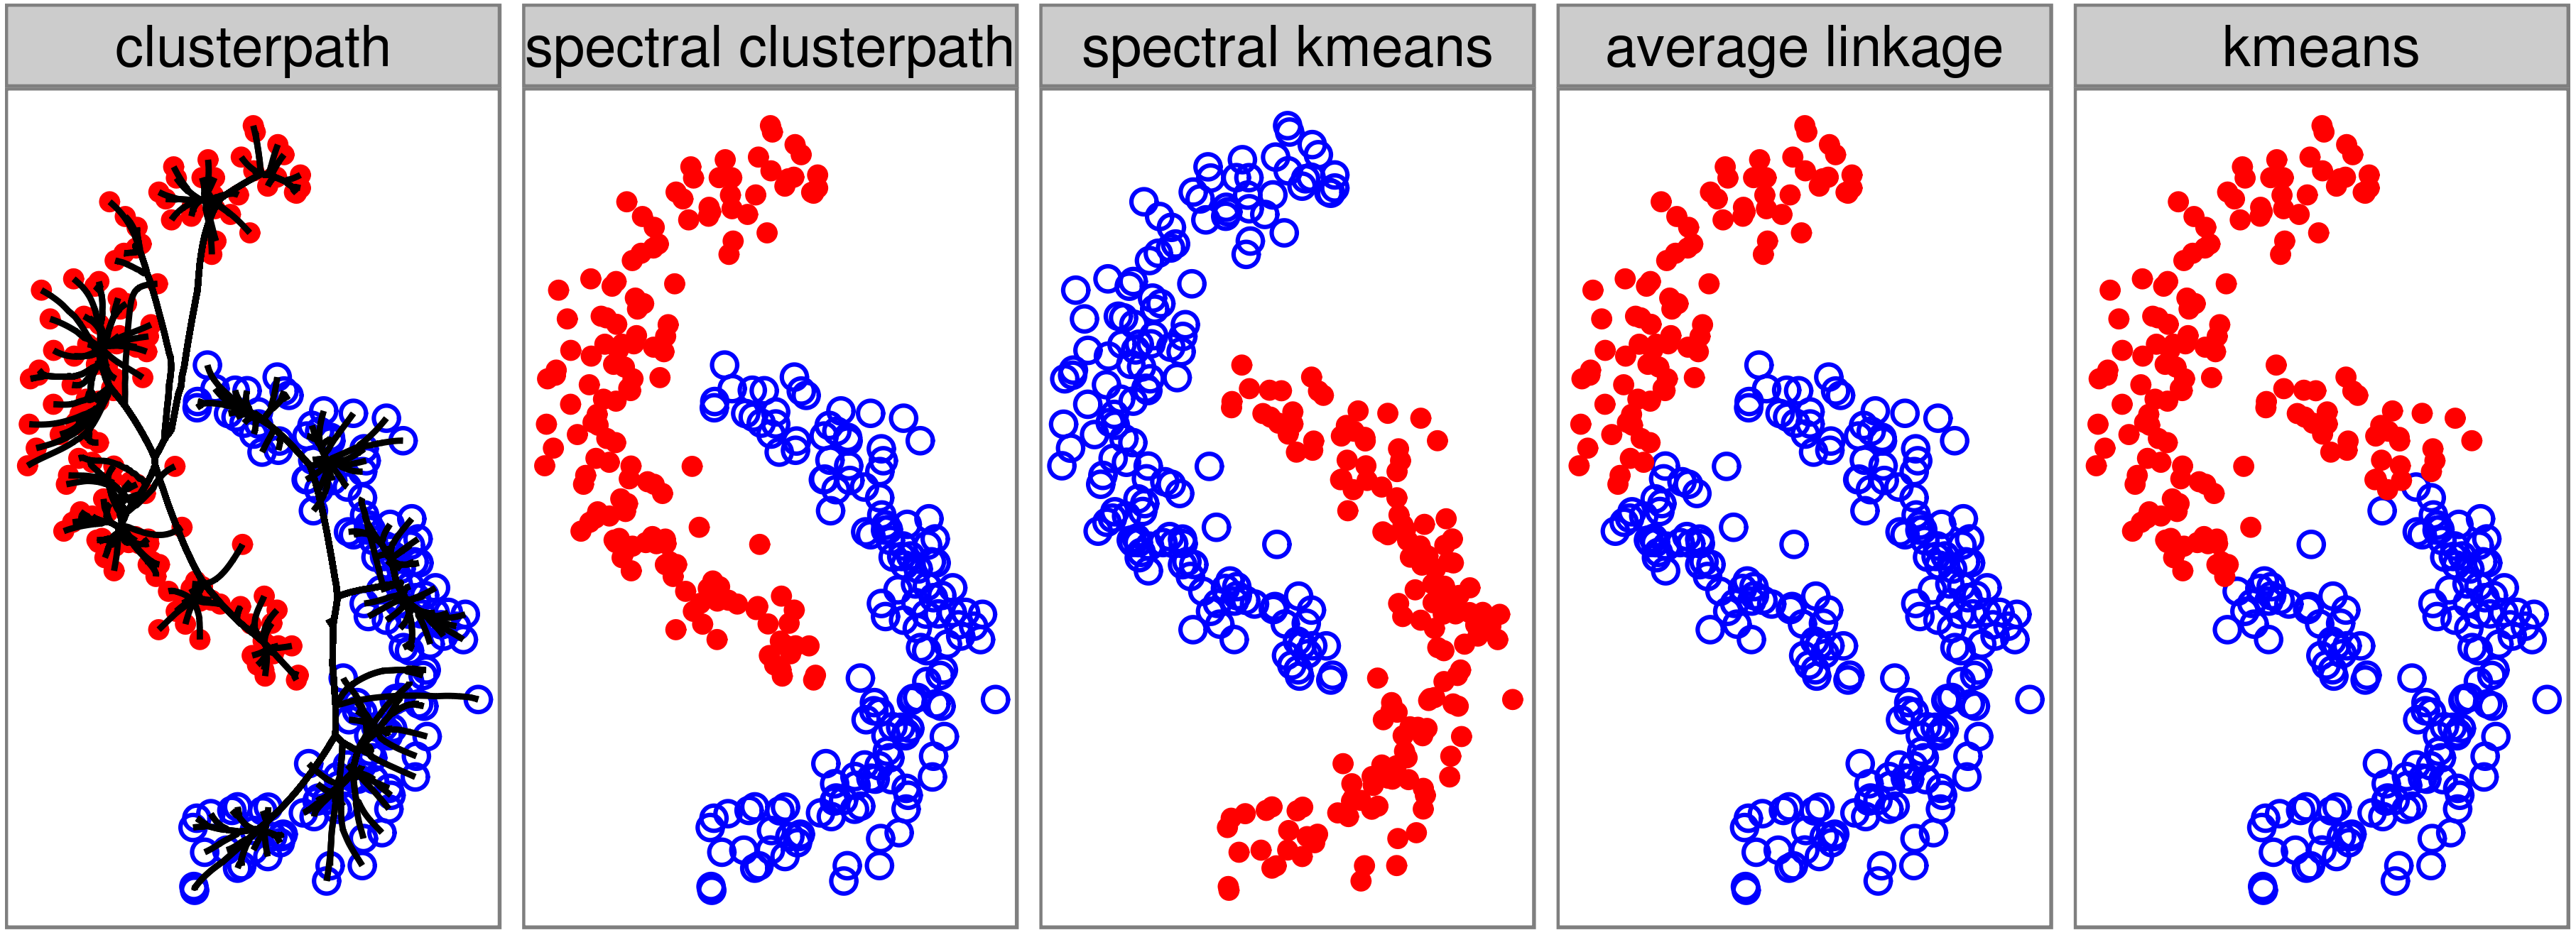
\includegraphics[width=0.3\paperwidth]{moons}

The weighted $\ell_2$ clusterpath applied to the iris data:
\includegraphics{iris-clusterpath}
% Created by tikzDevice version 0.5.3 on 2011-05-02 14:31:11
\begin{tikzpicture}[x=1pt,y=1pt]
\draw[color=white,opacity=0] (0,0) rectangle (289.08,361.35);
\begin{scope}
\path[clip] (  0.00,  0.00) rectangle (289.08,361.35);
\end{scope}
\begin{scope}
\path[clip] (  0.00,  0.00) rectangle (289.08,361.35);
\end{scope}
\begin{scope}
\path[clip] (  0.00,  0.00) rectangle (289.08,361.35);
\end{scope}
\begin{scope}
\path[clip] (  0.00,  0.00) rectangle (289.08,361.35);
\end{scope}
\begin{scope}
\path[clip] (  0.00,  0.00) rectangle (289.08,361.35);
\end{scope}
\begin{scope}
\path[clip] (  0.00,  0.00) rectangle (289.08,361.35);
\end{scope}
\begin{scope}
\path[clip] (  0.00,  0.00) rectangle (289.08,361.35);
\end{scope}
\begin{scope}
\path[clip] (  0.00,  0.00) rectangle (289.08,361.35);
\end{scope}
\begin{scope}
\path[clip] (  0.00,  0.00) rectangle (289.08,361.35);
\end{scope}
\begin{scope}
\path[clip] (  0.00,  0.00) rectangle (289.08,361.35);
\end{scope}
\begin{scope}
\path[clip] (  0.00,  0.00) rectangle (289.08,361.35);
\end{scope}
\begin{scope}
\path[clip] (  0.00,  0.00) rectangle (289.08,361.35);
\end{scope}
\begin{scope}
\path[clip] (  0.00,  0.00) rectangle (289.08,361.35);
\end{scope}
\begin{scope}
\path[clip] (  0.00,  0.00) rectangle (289.08,361.35);
\end{scope}
\begin{scope}
\path[clip] (  0.00,  0.00) rectangle (289.08,361.35);
\end{scope}
\begin{scope}
\path[clip] (  0.00,  0.00) rectangle (289.08,361.35);
\end{scope}
\begin{scope}
\path[clip] (  0.00,  0.00) rectangle (289.08,361.35);
\end{scope}
\begin{scope}
\path[clip] (  0.00,  0.00) rectangle (289.08,361.35);
\end{scope}
\begin{scope}
\path[clip] (  0.00,  0.00) rectangle (289.08,361.35);
\end{scope}
\begin{scope}
\path[clip] (  0.00,  0.00) rectangle (289.08,361.35);
\end{scope}
\begin{scope}
\path[clip] (  0.00,  0.00) rectangle (289.08,361.35);

\draw[fill opacity=0.00,draw opacity=0.00,] (  0.00,  0.00) rectangle (289.08,361.35);
\end{scope}
\begin{scope}
\path[clip] (  0.00,  0.00) rectangle (289.08,361.35);
\end{scope}
\begin{scope}
\path[clip] (  0.00,  0.00) rectangle (289.08,361.35);
\end{scope}
\begin{scope}
\path[clip] (  0.00,  0.00) rectangle (289.08,361.35);
\end{scope}
\begin{scope}
\path[clip] (  0.00,  0.00) rectangle (289.08,361.35);
\end{scope}
\begin{scope}
\path[clip] (  0.00,  0.00) rectangle (289.08,361.35);
\end{scope}
\begin{scope}
\path[clip] (  0.00,  0.00) rectangle (289.08,361.35);
\definecolor[named]{drawColor}{rgb}{0.00,0.00,0.00}

\node[color=drawColor,anchor=base,inner sep=0pt, outer sep=0pt, scale=  1.00] at (112.89, 14.45) {Number of clusters%
};
\end{scope}
\begin{scope}
\path[clip] (  0.00,  0.00) rectangle (289.08,361.35);
\end{scope}
\begin{scope}
\path[clip] (  0.00,  0.00) rectangle (289.08,361.35);
\end{scope}
\begin{scope}
\path[clip] (  0.00,  0.00) rectangle (289.08,361.35);
\definecolor[named]{drawColor}{rgb}{0.00,0.00,0.00}

\node[rotate= 90.00,color=drawColor,anchor=base,inner sep=0pt, outer sep=0pt, scale=  1.00] at ( 19.11,184.81) {Normalized Rand index (bigger means better agreement with known clusters)%
};
\end{scope}
\begin{scope}
\path[clip] (  0.00,  0.00) rectangle (289.08,361.35);
\end{scope}
\begin{scope}
\path[clip] (  0.00,  0.00) rectangle (289.08,361.35);
\end{scope}
\begin{scope}
\path[clip] (  0.00,  0.00) rectangle (289.08,361.35);
\end{scope}
\begin{scope}
\path[clip] ( 22.72,346.90) rectangle ( 46.29,346.90);
\end{scope}
\begin{scope}
\path[clip] (  0.00,  0.00) rectangle (289.08,361.35);
\end{scope}
\begin{scope}
\path[clip] ( 22.72,346.90) rectangle ( 46.29,346.90);
\end{scope}
\begin{scope}
\path[clip] (  0.00,  0.00) rectangle (289.08,361.35);
\end{scope}
\begin{scope}
\path[clip] (  0.00,  0.00) rectangle (289.08,361.35);
\end{scope}
\begin{scope}
\path[clip] (  0.00,  0.00) rectangle (289.08,361.35);
\end{scope}
\begin{scope}
\path[clip] ( 22.72,192.09) rectangle ( 46.29,195.70);
\end{scope}
\begin{scope}
\path[clip] (  0.00,  0.00) rectangle (289.08,361.35);
\end{scope}
\begin{scope}
\path[clip] (  0.00,  0.00) rectangle (289.08,361.35);
\end{scope}
\begin{scope}
\path[clip] (  0.00,  0.00) rectangle (289.08,361.35);
\end{scope}
\begin{scope}
\path[clip] ( 22.72, 40.89) rectangle ( 46.29, 40.89);
\end{scope}
\begin{scope}
\path[clip] (  0.00,  0.00) rectangle (289.08,361.35);
\end{scope}
\begin{scope}
\path[clip] ( 22.72, 22.72) rectangle ( 46.29, 40.89);
\end{scope}
\begin{scope}
\path[clip] (  0.00,  0.00) rectangle (289.08,361.35);
\end{scope}
\begin{scope}
\path[clip] ( 22.72, 22.72) rectangle ( 46.29, 22.72);
\end{scope}
\begin{scope}
\path[clip] (  0.00,  0.00) rectangle (289.08,361.35);
\end{scope}
\begin{scope}
\path[clip] ( 46.29,346.90) rectangle ( 46.29,346.90);
\end{scope}
\begin{scope}
\path[clip] (  0.00,  0.00) rectangle (289.08,361.35);
\end{scope}
\begin{scope}
\path[clip] ( 46.29,346.90) rectangle ( 46.29,346.90);
\end{scope}
\begin{scope}
\path[clip] (  0.00,  0.00) rectangle (289.08,361.35);
\end{scope}
\begin{scope}
\path[clip] ( 46.29,195.70) rectangle ( 46.29,346.90);
\end{scope}
\begin{scope}
\path[clip] (  0.00,  0.00) rectangle (289.08,361.35);
\end{scope}
\begin{scope}
\path[clip] ( 46.29,192.09) rectangle ( 46.29,195.70);
\end{scope}
\begin{scope}
\path[clip] (  0.00,  0.00) rectangle (289.08,361.35);
\end{scope}
\begin{scope}
\path[clip] ( 46.29, 40.89) rectangle ( 46.29,192.09);
\end{scope}
\begin{scope}
\path[clip] (  0.00,  0.00) rectangle (289.08,361.35);
\end{scope}
\begin{scope}
\path[clip] ( 46.29, 40.89) rectangle ( 46.29, 40.89);
\end{scope}
\begin{scope}
\path[clip] (  0.00,  0.00) rectangle (289.08,361.35);
\end{scope}
\begin{scope}
\path[clip] ( 46.29, 22.72) rectangle ( 46.29, 40.89);
\end{scope}
\begin{scope}
\path[clip] (  0.00,  0.00) rectangle (289.08,361.35);
\end{scope}
\begin{scope}
\path[clip] ( 46.29, 22.72) rectangle ( 46.29, 22.72);
\end{scope}
\begin{scope}
\path[clip] (  0.00,  0.00) rectangle (289.08,361.35);
\end{scope}
\begin{scope}
\path[clip] ( 46.29,346.90) rectangle (189.23,346.90);
\end{scope}
\begin{scope}
\path[clip] (  0.00,  0.00) rectangle (289.08,361.35);
\end{scope}
\begin{scope}
\path[clip] ( 46.29,346.90) rectangle (189.23,346.90);
\end{scope}
\begin{scope}
\path[clip] (  0.00,  0.00) rectangle (289.08,361.35);
\end{scope}
\begin{scope}
\path[clip] ( 46.29,195.70) rectangle (189.23,346.90);
\end{scope}
\begin{scope}
\path[clip] (  0.00,  0.00) rectangle (289.08,361.35);
\end{scope}
\begin{scope}
\path[clip] ( 46.29,192.09) rectangle (189.23,195.70);
\end{scope}
\begin{scope}
\path[clip] (  0.00,  0.00) rectangle (289.08,361.35);
\end{scope}
\begin{scope}
\path[clip] ( 46.29, 40.89) rectangle (189.23,192.09);
\end{scope}
\begin{scope}
\path[clip] (  0.00,  0.00) rectangle (289.08,361.35);
\end{scope}
\begin{scope}
\path[clip] ( 46.29, 40.89) rectangle (189.23, 40.89);
\end{scope}
\begin{scope}
\path[clip] (  0.00,  0.00) rectangle (289.08,361.35);
\end{scope}
\begin{scope}
\path[clip] (  0.00,  0.00) rectangle (289.08,361.35);
\end{scope}
\begin{scope}
\path[clip] (  0.00,  0.00) rectangle (289.08,361.35);
\end{scope}
\begin{scope}
\path[clip] ( 46.29, 22.72) rectangle (189.23, 22.72);
\end{scope}
\begin{scope}
\path[clip] (  0.00,  0.00) rectangle (289.08,361.35);
\end{scope}
\begin{scope}
\path[clip] (189.23,346.90) rectangle (189.23,346.90);
\end{scope}
\begin{scope}
\path[clip] (  0.00,  0.00) rectangle (289.08,361.35);
\end{scope}
\begin{scope}
\path[clip] (189.23,346.90) rectangle (189.23,346.90);
\end{scope}
\begin{scope}
\path[clip] (  0.00,  0.00) rectangle (289.08,361.35);
\end{scope}
\begin{scope}
\path[clip] (189.23,195.70) rectangle (189.23,346.90);
\end{scope}
\begin{scope}
\path[clip] (  0.00,  0.00) rectangle (289.08,361.35);
\end{scope}
\begin{scope}
\path[clip] (189.23,192.09) rectangle (189.23,195.70);
\end{scope}
\begin{scope}
\path[clip] (  0.00,  0.00) rectangle (289.08,361.35);
\end{scope}
\begin{scope}
\path[clip] (189.23, 40.89) rectangle (189.23,192.09);
\end{scope}
\begin{scope}
\path[clip] (  0.00,  0.00) rectangle (289.08,361.35);
\end{scope}
\begin{scope}
\path[clip] (189.23, 40.89) rectangle (189.23, 40.89);
\end{scope}
\begin{scope}
\path[clip] (  0.00,  0.00) rectangle (289.08,361.35);
\end{scope}
\begin{scope}
\path[clip] (189.23, 22.72) rectangle (189.23, 40.89);
\end{scope}
\begin{scope}
\path[clip] (  0.00,  0.00) rectangle (289.08,361.35);
\end{scope}
\begin{scope}
\path[clip] (189.23, 22.72) rectangle (189.23, 22.72);
\end{scope}
\begin{scope}
\path[clip] (  0.00,  0.00) rectangle (289.08,361.35);
\end{scope}
\begin{scope}
\path[clip] (189.23,346.90) rectangle (203.07,346.90);
\end{scope}
\begin{scope}
\path[clip] (  0.00,  0.00) rectangle (289.08,361.35);
\end{scope}
\begin{scope}
\path[clip] (189.23,346.90) rectangle (203.07,346.90);
\end{scope}
\begin{scope}
\path[clip] (  0.00,  0.00) rectangle (289.08,361.35);
\end{scope}
\begin{scope}
\path[clip] (189.23,195.70) rectangle (203.07,346.90);
\end{scope}
\begin{scope}
\path[clip] (  0.00,  0.00) rectangle (289.08,361.35);
\end{scope}
\begin{scope}
\path[clip] (189.23,192.09) rectangle (203.07,195.70);
\end{scope}
\begin{scope}
\path[clip] (  0.00,  0.00) rectangle (289.08,361.35);
\end{scope}
\begin{scope}
\path[clip] (189.23, 40.89) rectangle (203.07,192.09);
\end{scope}
\begin{scope}
\path[clip] (  0.00,  0.00) rectangle (289.08,361.35);
\end{scope}
\begin{scope}
\path[clip] (189.23, 40.89) rectangle (203.07, 40.89);
\end{scope}
\begin{scope}
\path[clip] (  0.00,  0.00) rectangle (289.08,361.35);
\end{scope}
\begin{scope}
\path[clip] (189.23, 22.72) rectangle (203.07, 40.89);
\end{scope}
\begin{scope}
\path[clip] (  0.00,  0.00) rectangle (289.08,361.35);
\end{scope}
\begin{scope}
\path[clip] (189.23, 22.72) rectangle (203.07, 22.72);
\end{scope}
\begin{scope}
\path[clip] (  0.00,  0.00) rectangle (289.08,361.35);
\end{scope}
\begin{scope}
\path[clip] (203.07,346.90) rectangle (203.07,346.90);
\end{scope}
\begin{scope}
\path[clip] (  0.00,  0.00) rectangle (289.08,361.35);
\end{scope}
\begin{scope}
\path[clip] (203.07,346.90) rectangle (203.07,346.90);
\end{scope}
\begin{scope}
\path[clip] (  0.00,  0.00) rectangle (289.08,361.35);
\end{scope}
\begin{scope}
\path[clip] (203.07,195.70) rectangle (203.07,346.90);
\end{scope}
\begin{scope}
\path[clip] (  0.00,  0.00) rectangle (289.08,361.35);
\end{scope}
\begin{scope}
\path[clip] (203.07,192.09) rectangle (203.07,195.70);
\end{scope}
\begin{scope}
\path[clip] (  0.00,  0.00) rectangle (289.08,361.35);
\end{scope}
\begin{scope}
\path[clip] (203.07, 40.89) rectangle (203.07,192.09);
\end{scope}
\begin{scope}
\path[clip] (  0.00,  0.00) rectangle (289.08,361.35);
\end{scope}
\begin{scope}
\path[clip] (203.07, 40.89) rectangle (203.07, 40.89);
\end{scope}
\begin{scope}
\path[clip] (  0.00,  0.00) rectangle (289.08,361.35);
\end{scope}
\begin{scope}
\path[clip] (203.07, 22.72) rectangle (203.07, 40.89);
\end{scope}
\begin{scope}
\path[clip] (  0.00,  0.00) rectangle (289.08,361.35);
\end{scope}
\begin{scope}
\path[clip] (203.07, 22.72) rectangle (203.07, 22.72);
\end{scope}
\begin{scope}
\path[clip] (  0.00,  0.00) rectangle (289.08,361.35);
\end{scope}
\begin{scope}
\path[clip] ( 22.72,346.90) rectangle ( 46.29,346.90);
\end{scope}
\begin{scope}
\path[clip] (  0.00,  0.00) rectangle (289.08,361.35);
\end{scope}
\begin{scope}
\path[clip] ( 22.72,346.90) rectangle ( 46.29,346.90);
\end{scope}
\begin{scope}
\path[clip] (  0.00,  0.00) rectangle (289.08,361.35);
\end{scope}
\begin{scope}
\path[clip] (  0.00,  0.00) rectangle (289.08,361.35);
\definecolor[named]{drawColor}{rgb}{0.00,0.00,0.00}

\draw[color=drawColor,line width= 0.0pt,line cap=round,line join=round,fill opacity=0.00,] ( 41.95,233.50) -- ( 46.29,233.50);

\draw[color=drawColor,line width= 0.0pt,line cap=round,line join=round,fill opacity=0.00,] ( 41.95,271.30) -- ( 46.29,271.30);

\draw[color=drawColor,line width= 0.0pt,line cap=round,line join=round,fill opacity=0.00,] ( 41.95,309.10) -- ( 46.29,309.10);

\draw[color=drawColor,line width= 0.0pt,line cap=round,line join=round,fill opacity=0.00,] ( 41.95,346.90) -- ( 46.29,346.90);

\node[color=drawColor,anchor=base east,inner sep=0pt, outer sep=0pt, scale=  0.80] at ( 39.35,230.19) {0.4%
};

\node[color=drawColor,anchor=base east,inner sep=0pt, outer sep=0pt, scale=  0.80] at ( 39.35,267.99) {0.6%
};

\node[color=drawColor,anchor=base east,inner sep=0pt, outer sep=0pt, scale=  0.80] at ( 39.35,305.79) {0.8%
};

\node[color=drawColor,anchor=base east,inner sep=0pt, outer sep=0pt, scale=  0.80] at ( 39.35,343.59) {1.0%
};
\end{scope}
\begin{scope}
\path[clip] (  0.00,  0.00) rectangle (289.08,361.35);
\end{scope}
\begin{scope}
\path[clip] ( 22.72,192.09) rectangle ( 46.29,195.70);
\end{scope}
\begin{scope}
\path[clip] (  0.00,  0.00) rectangle (289.08,361.35);
\end{scope}
\begin{scope}
\path[clip] (  0.00,  0.00) rectangle (289.08,361.35);
\definecolor[named]{drawColor}{rgb}{0.00,0.00,0.00}

\draw[color=drawColor,line width= 0.0pt,line cap=round,line join=round,fill opacity=0.00,] ( 41.95, 78.69) -- ( 46.29, 78.69);

\draw[color=drawColor,line width= 0.0pt,line cap=round,line join=round,fill opacity=0.00,] ( 41.95,116.49) -- ( 46.29,116.49);

\draw[color=drawColor,line width= 0.0pt,line cap=round,line join=round,fill opacity=0.00,] ( 41.95,154.29) -- ( 46.29,154.29);

\draw[color=drawColor,line width= 0.0pt,line cap=round,line join=round,fill opacity=0.00,] ( 41.95,192.09) -- ( 46.29,192.09);

\node[color=drawColor,anchor=base east,inner sep=0pt, outer sep=0pt, scale=  0.80] at ( 39.35, 75.39) {0.4%
};

\node[color=drawColor,anchor=base east,inner sep=0pt, outer sep=0pt, scale=  0.80] at ( 39.35,113.18) {0.6%
};

\node[color=drawColor,anchor=base east,inner sep=0pt, outer sep=0pt, scale=  0.80] at ( 39.35,150.98) {0.8%
};

\node[color=drawColor,anchor=base east,inner sep=0pt, outer sep=0pt, scale=  0.80] at ( 39.35,188.78) {1.0%
};
\end{scope}
\begin{scope}
\path[clip] (  0.00,  0.00) rectangle (289.08,361.35);
\end{scope}
\begin{scope}
\path[clip] ( 22.72, 40.89) rectangle ( 46.29, 40.89);
\end{scope}
\begin{scope}
\path[clip] (  0.00,  0.00) rectangle (289.08,361.35);
\end{scope}
\begin{scope}
\path[clip] ( 22.72, 22.72) rectangle ( 46.29, 40.89);
\end{scope}
\begin{scope}
\path[clip] (  0.00,  0.00) rectangle (289.08,361.35);
\end{scope}
\begin{scope}
\path[clip] ( 22.72, 22.72) rectangle ( 46.29, 22.72);
\end{scope}
\begin{scope}
\path[clip] (  0.00,  0.00) rectangle (289.08,361.35);
\end{scope}
\begin{scope}
\path[clip] ( 46.29,346.90) rectangle ( 46.29,346.90);
\end{scope}
\begin{scope}
\path[clip] (  0.00,  0.00) rectangle (289.08,361.35);
\end{scope}
\begin{scope}
\path[clip] ( 46.29,346.90) rectangle ( 46.29,346.90);
\end{scope}
\begin{scope}
\path[clip] (  0.00,  0.00) rectangle (289.08,361.35);
\end{scope}
\begin{scope}
\path[clip] ( 46.29,195.70) rectangle ( 46.29,346.90);
\end{scope}
\begin{scope}
\path[clip] (  0.00,  0.00) rectangle (289.08,361.35);
\end{scope}
\begin{scope}
\path[clip] ( 46.29,192.09) rectangle ( 46.29,195.70);
\end{scope}
\begin{scope}
\path[clip] (  0.00,  0.00) rectangle (289.08,361.35);
\end{scope}
\begin{scope}
\path[clip] ( 46.29, 40.89) rectangle ( 46.29,192.09);
\end{scope}
\begin{scope}
\path[clip] (  0.00,  0.00) rectangle (289.08,361.35);
\end{scope}
\begin{scope}
\path[clip] ( 46.29, 40.89) rectangle ( 46.29, 40.89);
\end{scope}
\begin{scope}
\path[clip] (  0.00,  0.00) rectangle (289.08,361.35);
\end{scope}
\begin{scope}
\path[clip] ( 46.29, 22.72) rectangle ( 46.29, 40.89);
\end{scope}
\begin{scope}
\path[clip] (  0.00,  0.00) rectangle (289.08,361.35);
\end{scope}
\begin{scope}
\path[clip] ( 46.29, 22.72) rectangle ( 46.29, 22.72);
\end{scope}
\begin{scope}
\path[clip] (  0.00,  0.00) rectangle (289.08,361.35);
\end{scope}
\begin{scope}
\path[clip] ( 46.29,346.90) rectangle (189.23,346.90);
\end{scope}
\begin{scope}
\path[clip] (  0.00,  0.00) rectangle (289.08,361.35);
\end{scope}
\begin{scope}
\path[clip] ( 46.29,346.90) rectangle (189.23,346.90);
\end{scope}
\begin{scope}
\path[clip] (  0.00,  0.00) rectangle (289.08,361.35);
\end{scope}
\begin{scope}
\path[clip] ( 46.29,195.70) rectangle (189.23,346.90);
\definecolor[named]{fillColor}{rgb}{1.00,1.00,1.00}

\draw[fill=fillColor,draw opacity=0.00,] ( 46.29,195.70) rectangle (189.23,346.90);
\definecolor[named]{drawColor}{rgb}{0.98,0.98,0.98}

\draw[color=drawColor,line cap=round,line join=round,fill opacity=0.00,] ( 46.29,195.70) --
	(189.23,195.70);

\draw[color=drawColor,line cap=round,line join=round,fill opacity=0.00,] ( 46.29,214.60) --
	(189.23,214.60);

\draw[color=drawColor,line cap=round,line join=round,fill opacity=0.00,] ( 46.29,233.50) --
	(189.23,233.50);

\draw[color=drawColor,line cap=round,line join=round,fill opacity=0.00,] ( 46.29,252.40) --
	(189.23,252.40);

\draw[color=drawColor,line cap=round,line join=round,fill opacity=0.00,] ( 46.29,271.30) --
	(189.23,271.30);

\draw[color=drawColor,line cap=round,line join=round,fill opacity=0.00,] ( 46.29,290.20) --
	(189.23,290.20);

\draw[color=drawColor,line cap=round,line join=round,fill opacity=0.00,] ( 46.29,309.10) --
	(189.23,309.10);

\draw[color=drawColor,line cap=round,line join=round,fill opacity=0.00,] ( 46.29,328.00) --
	(189.23,328.00);

\draw[color=drawColor,line cap=round,line join=round,fill opacity=0.00,] ( 46.29,346.90) --
	(189.23,346.90);

\draw[color=drawColor,line cap=round,line join=round,fill opacity=0.00,] ( 46.29,195.70) --
	( 46.29,346.90);

\draw[color=drawColor,line cap=round,line join=round,fill opacity=0.00,] ( 54.23,195.70) --
	( 54.23,346.90);

\draw[color=drawColor,line cap=round,line join=round,fill opacity=0.00,] ( 62.17,195.70) --
	( 62.17,346.90);

\draw[color=drawColor,line cap=round,line join=round,fill opacity=0.00,] ( 78.05,195.70) --
	( 78.05,346.90);

\draw[color=drawColor,line cap=round,line join=round,fill opacity=0.00,] ( 93.94,195.70) --
	( 93.94,346.90);

\draw[color=drawColor,line cap=round,line join=round,fill opacity=0.00,] (133.64,195.70) --
	(133.64,346.90);

\draw[color=drawColor,line cap=round,line join=round,fill opacity=0.00,] (173.35,195.70) --
	(173.35,346.90);
\definecolor[named]{drawColor}{rgb}{0.90,0.90,0.90}

\draw[color=drawColor,line width= 0.0pt,line cap=round,line join=round,fill opacity=0.00,] ( 46.29,233.50) --
	(189.23,233.50);

\draw[color=drawColor,line width= 0.0pt,line cap=round,line join=round,fill opacity=0.00,] ( 46.29,271.30) --
	(189.23,271.30);

\draw[color=drawColor,line width= 0.0pt,line cap=round,line join=round,fill opacity=0.00,] ( 46.29,309.10) --
	(189.23,309.10);

\draw[color=drawColor,line width= 0.0pt,line cap=round,line join=round,fill opacity=0.00,] ( 46.29,346.90) --
	(189.23,346.90);

\draw[color=drawColor,line width= 0.0pt,line cap=round,line join=round,fill opacity=0.00,] ( 46.29,195.70) --
	( 46.29,346.90);

\draw[color=drawColor,line width= 0.0pt,line cap=round,line join=round,fill opacity=0.00,] ( 62.17,195.70) --
	( 62.17,346.90);

\draw[color=drawColor,line width= 0.0pt,line cap=round,line join=round,fill opacity=0.00,] ( 93.94,195.70) --
	( 93.94,346.90);

\draw[color=drawColor,line width= 0.0pt,line cap=round,line join=round,fill opacity=0.00,] (173.35,195.70) --
	(173.35,346.90);
\definecolor[named]{drawColor}{rgb}{0.97,0.46,0.43}

\draw[color=drawColor,line width= 2.0pt,line join=round,fill opacity=0.00,] ( 46.29,265.27) --
	( 62.17,263.43) --
	( 78.05,262.27) --
	( 93.94,262.19) --
	(109.82,261.83) --
	(125.70,261.23) --
	(141.58,259.77) --
	(157.46,257.96) --
	(173.35,255.95) --
	(189.23,255.65);
\definecolor[named]{drawColor}{rgb}{0.72,0.62,0.00}

\draw[color=drawColor,line width= 2.0pt,dash pattern=on 2pt off 2pt ,line join=round,fill opacity=0.00,] ( 46.29,265.27) --
	( 62.17,263.43) --
	( 78.05,262.58) --
	( 93.94,260.74) --
	(109.82,260.20) --
	(125.70,259.77) --
	(141.58,259.36) --
	(157.46,259.32) --
	(173.35,258.24) --
	(189.23,256.37);
\definecolor[named]{drawColor}{rgb}{0.00,0.73,0.22}

\draw[color=drawColor,line width= 2.0pt,dash pattern=on 4pt off 2pt ,line join=round,fill opacity=0.00,] ( 46.29,265.27) --
	( 62.17,263.43) --
	( 78.05,262.58) --
	( 93.94,262.19) --
	(109.82,261.63) --
	(125.70,259.77) --
	(141.58,259.36) --
	(157.46,258.47) --
	(173.35,258.03) --
	(189.23,255.63);
\definecolor[named]{drawColor}{rgb}{0.00,0.75,0.77}

\draw[color=drawColor,line width= 2.0pt,dash pattern=on 4pt off 4pt ,line join=round,fill opacity=0.00,] ( 46.29,265.27) --
	( 62.17,328.73) --
	( 78.05,243.42) --
	( 93.94,305.57) --
	(109.82,281.69) --
	(125.70,270.95) --
	(141.58,250.13) --
	(157.46,237.41) --
	(173.35,232.85) --
	(189.23,231.46);
\definecolor[named]{drawColor}{rgb}{0.38,0.61,1.00}

\draw[color=drawColor,line width= 2.0pt,dash pattern=on 1pt off 3pt ,line join=round,fill opacity=0.00,] ( 46.29,265.27) --
	( 62.17,264.14) --
	( 78.05,262.27) --
	( 93.94,262.02) --
	(109.82,254.27) --
	(125.70,262.55) --
	(141.58,254.36) --
	(157.46,252.62) --
	(173.35,228.34) --
	(189.23,234.05);
\definecolor[named]{drawColor}{rgb}{0.96,0.39,0.89}

\draw[color=drawColor,line width= 2.0pt,dash pattern=on 1pt off 3pt on 4pt off 3pt ,line join=round,fill opacity=0.00,] ( 46.29,265.27) --
	( 62.17,266.69) --
	( 78.05,257.27) --
	( 93.94,248.43) --
	(109.82,240.30) --
	(125.70,235.60) --
	(141.58,232.24) --
	(157.46,227.93) --
	(173.35,223.60) --
	(189.23,220.48);

\draw[color=drawColor,line width= 2.0pt,dash pattern=on 1pt off 3pt on 4pt off 3pt ,line join=round,fill opacity=0.00,] ( 46.29,265.27) -- ( 46.29,265.27);

\draw[color=drawColor,line width= 2.0pt,dash pattern=on 1pt off 3pt on 4pt off 3pt ,line join=round,fill opacity=0.00,] ( 62.17,252.00) -- ( 62.17,281.38);

\draw[color=drawColor,line width= 2.0pt,dash pattern=on 1pt off 3pt on 4pt off 3pt ,line join=round,fill opacity=0.00,] ( 78.05,249.16) -- ( 78.05,265.38);

\draw[color=drawColor,line width= 2.0pt,dash pattern=on 1pt off 3pt on 4pt off 3pt ,line join=round,fill opacity=0.00,] ( 93.94,235.55) -- ( 93.94,261.31);

\draw[color=drawColor,line width= 2.0pt,dash pattern=on 1pt off 3pt on 4pt off 3pt ,line join=round,fill opacity=0.00,] (109.82,226.64) -- (109.82,253.96);

\draw[color=drawColor,line width= 2.0pt,dash pattern=on 1pt off 3pt on 4pt off 3pt ,line join=round,fill opacity=0.00,] (125.70,220.21) -- (125.70,250.99);

\draw[color=drawColor,line width= 2.0pt,dash pattern=on 1pt off 3pt on 4pt off 3pt ,line join=round,fill opacity=0.00,] (141.58,216.87) -- (141.58,247.60);

\draw[color=drawColor,line width= 2.0pt,dash pattern=on 1pt off 3pt on 4pt off 3pt ,line join=round,fill opacity=0.00,] (157.46,213.94) -- (157.46,241.91);

\draw[color=drawColor,line width= 2.0pt,dash pattern=on 1pt off 3pt on 4pt off 3pt ,line join=round,fill opacity=0.00,] (173.35,211.10) -- (173.35,236.10);

\draw[color=drawColor,line width= 2.0pt,dash pattern=on 1pt off 3pt on 4pt off 3pt ,line join=round,fill opacity=0.00,] (189.23,208.57) -- (189.23,232.39);
\definecolor[named]{drawColor}{rgb}{0.50,0.50,0.50}

\draw[color=drawColor,line cap=round,line join=round,fill opacity=0.00,] ( 46.29,195.70) rectangle (189.23,346.90);
\end{scope}
\begin{scope}
\path[clip] (  0.00,  0.00) rectangle (289.08,361.35);
\end{scope}
\begin{scope}
\path[clip] ( 46.29,192.09) rectangle (189.23,195.70);
\end{scope}
\begin{scope}
\path[clip] (  0.00,  0.00) rectangle (289.08,361.35);
\end{scope}
\begin{scope}
\path[clip] ( 46.29, 40.89) rectangle (189.23,192.09);
\definecolor[named]{fillColor}{rgb}{1.00,1.00,1.00}

\draw[fill=fillColor,draw opacity=0.00,] ( 46.29, 40.89) rectangle (189.23,192.09);
\definecolor[named]{drawColor}{rgb}{0.98,0.98,0.98}

\draw[color=drawColor,line cap=round,line join=round,fill opacity=0.00,] ( 46.29, 40.89) --
	(189.23, 40.89);

\draw[color=drawColor,line cap=round,line join=round,fill opacity=0.00,] ( 46.29, 59.79) --
	(189.23, 59.79);

\draw[color=drawColor,line cap=round,line join=round,fill opacity=0.00,] ( 46.29, 78.69) --
	(189.23, 78.69);

\draw[color=drawColor,line cap=round,line join=round,fill opacity=0.00,] ( 46.29, 97.59) --
	(189.23, 97.59);

\draw[color=drawColor,line cap=round,line join=round,fill opacity=0.00,] ( 46.29,116.49) --
	(189.23,116.49);

\draw[color=drawColor,line cap=round,line join=round,fill opacity=0.00,] ( 46.29,135.39) --
	(189.23,135.39);

\draw[color=drawColor,line cap=round,line join=round,fill opacity=0.00,] ( 46.29,154.29) --
	(189.23,154.29);

\draw[color=drawColor,line cap=round,line join=round,fill opacity=0.00,] ( 46.29,173.19) --
	(189.23,173.19);

\draw[color=drawColor,line cap=round,line join=round,fill opacity=0.00,] ( 46.29,192.09) --
	(189.23,192.09);

\draw[color=drawColor,line cap=round,line join=round,fill opacity=0.00,] ( 46.29, 40.89) --
	( 46.29,192.09);

\draw[color=drawColor,line cap=round,line join=round,fill opacity=0.00,] ( 54.23, 40.89) --
	( 54.23,192.09);

\draw[color=drawColor,line cap=round,line join=round,fill opacity=0.00,] ( 62.17, 40.89) --
	( 62.17,192.09);

\draw[color=drawColor,line cap=round,line join=round,fill opacity=0.00,] ( 78.05, 40.89) --
	( 78.05,192.09);

\draw[color=drawColor,line cap=round,line join=round,fill opacity=0.00,] ( 93.94, 40.89) --
	( 93.94,192.09);

\draw[color=drawColor,line cap=round,line join=round,fill opacity=0.00,] (133.64, 40.89) --
	(133.64,192.09);

\draw[color=drawColor,line cap=round,line join=round,fill opacity=0.00,] (173.35, 40.89) --
	(173.35,192.09);
\definecolor[named]{drawColor}{rgb}{0.90,0.90,0.90}

\draw[color=drawColor,line width= 0.0pt,line cap=round,line join=round,fill opacity=0.00,] ( 46.29, 78.69) --
	(189.23, 78.69);

\draw[color=drawColor,line width= 0.0pt,line cap=round,line join=round,fill opacity=0.00,] ( 46.29,116.49) --
	(189.23,116.49);

\draw[color=drawColor,line width= 0.0pt,line cap=round,line join=round,fill opacity=0.00,] ( 46.29,154.29) --
	(189.23,154.29);

\draw[color=drawColor,line width= 0.0pt,line cap=round,line join=round,fill opacity=0.00,] ( 46.29,192.09) --
	(189.23,192.09);

\draw[color=drawColor,line width= 0.0pt,line cap=round,line join=round,fill opacity=0.00,] ( 46.29, 40.89) --
	( 46.29,192.09);

\draw[color=drawColor,line width= 0.0pt,line cap=round,line join=round,fill opacity=0.00,] ( 62.17, 40.89) --
	( 62.17,192.09);

\draw[color=drawColor,line width= 0.0pt,line cap=round,line join=round,fill opacity=0.00,] ( 93.94, 40.89) --
	( 93.94,192.09);

\draw[color=drawColor,line width= 0.0pt,line cap=round,line join=round,fill opacity=0.00,] (173.35, 40.89) --
	(173.35,192.09);
\definecolor[named]{drawColor}{rgb}{0.97,0.46,0.43}

\draw[color=drawColor,line width= 2.0pt,line join=round,fill opacity=0.00,] ( 46.29,192.09) --
	( 62.17,190.83) --
	( 78.05,189.58) --
	( 93.94,158.73) --
	(109.82,136.95) --
	(125.70,120.07) --
	(141.58, 94.51) --
	(157.46, 94.21) --
	(173.35, 64.83) --
	(189.23, 61.58);
\definecolor[named]{drawColor}{rgb}{0.72,0.62,0.00}

\draw[color=drawColor,line width= 2.0pt,dash pattern=on 2pt off 2pt ,line join=round,fill opacity=0.00,] ( 46.29, 13.73) --
	( 62.17,144.42) --
	( 78.05,132.64) --
	( 93.94,131.87) --
	(109.82,131.65) --
	(125.70,122.97) --
	(141.58, 79.28) --
	(157.46, 79.27) --
	(173.35, 67.35);
\definecolor[named]{drawColor}{rgb}{0.00,0.73,0.22}

\draw[color=drawColor,line width= 2.0pt,dash pattern=on 4pt off 2pt ,line join=round,fill opacity=0.00,] ( 46.29,192.09) --
	( 62.17,160.98) --
	( 78.05,154.36) --
	( 93.94,107.16) --
	(109.82, 93.34) --
	(125.70, 67.83) --
	(141.58, 58.38) --
	(157.46, 56.71) --
	(173.35, 56.69) --
	(189.23, 56.39);
\definecolor[named]{drawColor}{rgb}{0.00,0.75,0.77}

\draw[color=drawColor,line width= 2.0pt,dash pattern=on 4pt off 4pt ,line join=round,fill opacity=0.00,] ( 46.29,106.30) --
	( 62.17, 45.06) --
	( 78.05, 96.26) --
	( 93.94, 81.92) --
	(109.82, 67.84) --
	(125.70, 57.84) --
	(141.58, 50.45) --
	(157.46, 45.51) --
	(173.35, 44.39) --
	(189.23, 42.52);
\definecolor[named]{drawColor}{rgb}{0.38,0.61,1.00}

\draw[color=drawColor,line width= 2.0pt,dash pattern=on 1pt off 3pt ,line join=round,fill opacity=0.00,] ( 46.29, 66.33) --
	( 62.17, 55.66) --
	( 78.05, 98.64) --
	( 93.94, 82.80) --
	(109.82, 68.94) --
	(125.70, 60.65) --
	(141.58, 52.24) --
	(157.46, 49.38) --
	(173.35, 46.18) --
	(189.23, 41.33);
\definecolor[named]{drawColor}{rgb}{0.96,0.39,0.89}

\draw[color=drawColor,line width= 2.0pt,dash pattern=on 1pt off 3pt on 4pt off 3pt ,line join=round,fill opacity=0.00,] ( 46.29, 60.52) --
	( 62.17, 57.67) --
	( 78.05, 58.80) --
	( 93.94, 57.74) --
	(109.82, 56.09) --
	(125.70, 53.06) --
	(141.58, 49.58) --
	(157.46, 45.86) --
	(173.35, 42.11) --
	(189.23, 39.09);

\draw[color=drawColor,line width= 2.0pt,dash pattern=on 1pt off 3pt on 4pt off 3pt ,line join=round,fill opacity=0.00,] ( 46.29, 60.52) -- ( 46.29, 60.52);

\draw[color=drawColor,line width= 2.0pt,dash pattern=on 1pt off 3pt on 4pt off 3pt ,line join=round,fill opacity=0.00,] ( 62.17, 55.96) -- ( 62.17, 59.38);

\draw[color=drawColor,line width= 2.0pt,dash pattern=on 1pt off 3pt on 4pt off 3pt ,line join=round,fill opacity=0.00,] ( 78.05, 56.01) -- ( 78.05, 61.59);

\draw[color=drawColor,line width= 2.0pt,dash pattern=on 1pt off 3pt on 4pt off 3pt ,line join=round,fill opacity=0.00,] ( 93.94, 52.93) -- ( 93.94, 62.56);

\draw[color=drawColor,line width= 2.0pt,dash pattern=on 1pt off 3pt on 4pt off 3pt ,line join=round,fill opacity=0.00,] (109.82, 51.15) -- (109.82, 61.02);

\draw[color=drawColor,line width= 2.0pt,dash pattern=on 1pt off 3pt on 4pt off 3pt ,line join=round,fill opacity=0.00,] (125.70, 49.20) -- (125.70, 56.92);

\draw[color=drawColor,line width= 2.0pt,dash pattern=on 1pt off 3pt on 4pt off 3pt ,line join=round,fill opacity=0.00,] (141.58, 46.63) -- (141.58, 52.54);

\draw[color=drawColor,line width= 2.0pt,dash pattern=on 1pt off 3pt on 4pt off 3pt ,line join=round,fill opacity=0.00,] (157.46, 43.80) -- (157.46, 47.91);

\draw[color=drawColor,line width= 2.0pt,dash pattern=on 1pt off 3pt on 4pt off 3pt ,line join=round,fill opacity=0.00,] (173.35, 41.33) -- (173.35, 42.88);

\draw[color=drawColor,line width= 2.0pt,dash pattern=on 1pt off 3pt on 4pt off 3pt ,line join=round,fill opacity=0.00,] (189.23, 37.64) -- (189.23, 40.53);
\definecolor[named]{drawColor}{rgb}{0.50,0.50,0.50}

\draw[color=drawColor,line cap=round,line join=round,fill opacity=0.00,] ( 46.29, 40.89) rectangle (189.23,192.09);
\end{scope}
\begin{scope}
\path[clip] (  0.00,  0.00) rectangle (289.08,361.35);
\end{scope}
\begin{scope}
\path[clip] ( 46.29, 40.89) rectangle (189.23, 40.89);
\end{scope}
\begin{scope}
\path[clip] (  0.00,  0.00) rectangle (289.08,361.35);
\end{scope}
\begin{scope}
\path[clip] (  0.00,  0.00) rectangle (289.08,361.35);
\definecolor[named]{drawColor}{rgb}{0.00,0.00,0.00}

\draw[color=drawColor,line width= 0.0pt,line cap=round,line join=round,fill opacity=0.00,] ( 46.29, 36.56) -- ( 46.29, 40.89);

\draw[color=drawColor,line width= 0.0pt,line cap=round,line join=round,fill opacity=0.00,] ( 62.17, 36.56) -- ( 62.17, 40.89);

\draw[color=drawColor,line width= 0.0pt,line cap=round,line join=round,fill opacity=0.00,] ( 93.94, 36.56) -- ( 93.94, 40.89);

\draw[color=drawColor,line width= 0.0pt,line cap=round,line join=round,fill opacity=0.00,] (173.35, 36.56) -- (173.35, 40.89);

\node[color=drawColor,anchor=base,inner sep=0pt, outer sep=0pt, scale=  0.80] at ( 46.29, 27.34) {2%
};

\node[color=drawColor,anchor=base,inner sep=0pt, outer sep=0pt, scale=  0.80] at ( 62.17, 27.34) {3%
};

\node[color=drawColor,anchor=base,inner sep=0pt, outer sep=0pt, scale=  0.80] at ( 93.94, 27.34) {5%
};

\node[color=drawColor,anchor=base,inner sep=0pt, outer sep=0pt, scale=  0.80] at (173.35, 27.34) {10%
};
\end{scope}
\begin{scope}
\path[clip] (  0.00,  0.00) rectangle (289.08,361.35);
\end{scope}
\begin{scope}
\path[clip] ( 46.29, 22.72) rectangle (189.23, 22.72);
\end{scope}
\begin{scope}
\path[clip] (  0.00,  0.00) rectangle (289.08,361.35);
\end{scope}
\begin{scope}
\path[clip] (189.23,346.90) rectangle (189.23,346.90);
\end{scope}
\begin{scope}
\path[clip] (  0.00,  0.00) rectangle (289.08,361.35);
\end{scope}
\begin{scope}
\path[clip] (189.23,346.90) rectangle (189.23,346.90);
\end{scope}
\begin{scope}
\path[clip] (  0.00,  0.00) rectangle (289.08,361.35);
\end{scope}
\begin{scope}
\path[clip] (189.23,195.70) rectangle (189.23,346.90);
\end{scope}
\begin{scope}
\path[clip] (  0.00,  0.00) rectangle (289.08,361.35);
\end{scope}
\begin{scope}
\path[clip] (189.23,192.09) rectangle (189.23,195.70);
\end{scope}
\begin{scope}
\path[clip] (  0.00,  0.00) rectangle (289.08,361.35);
\end{scope}
\begin{scope}
\path[clip] (189.23, 40.89) rectangle (189.23,192.09);
\end{scope}
\begin{scope}
\path[clip] (  0.00,  0.00) rectangle (289.08,361.35);
\end{scope}
\begin{scope}
\path[clip] (189.23, 40.89) rectangle (189.23, 40.89);
\end{scope}
\begin{scope}
\path[clip] (  0.00,  0.00) rectangle (289.08,361.35);
\end{scope}
\begin{scope}
\path[clip] (189.23, 22.72) rectangle (189.23, 40.89);
\end{scope}
\begin{scope}
\path[clip] (  0.00,  0.00) rectangle (289.08,361.35);
\end{scope}
\begin{scope}
\path[clip] (189.23, 22.72) rectangle (189.23, 22.72);
\end{scope}
\begin{scope}
\path[clip] (  0.00,  0.00) rectangle (289.08,361.35);
\end{scope}
\begin{scope}
\path[clip] (189.23,346.90) rectangle (203.07,346.90);
\end{scope}
\begin{scope}
\path[clip] (  0.00,  0.00) rectangle (289.08,361.35);
\end{scope}
\begin{scope}
\path[clip] (189.23,346.90) rectangle (203.07,346.90);
\end{scope}
\begin{scope}
\path[clip] (  0.00,  0.00) rectangle (289.08,361.35);
\end{scope}
\begin{scope}
\path[clip] (189.23,195.70) rectangle (203.07,346.90);
\definecolor[named]{drawColor}{rgb}{0.50,0.50,0.50}
\definecolor[named]{fillColor}{rgb}{0.80,0.80,0.80}

\draw[color=drawColor,line cap=round,line join=round,fill=fillColor,] (189.23,195.70) rectangle (203.07,346.90);
\definecolor[named]{drawColor}{rgb}{0.00,0.00,0.00}

\node[rotate=-90.00,color=drawColor,anchor=base,inner sep=0pt, outer sep=0pt, scale=  0.80] at (192.84,271.30) {data: iris%
};
\end{scope}
\begin{scope}
\path[clip] (  0.00,  0.00) rectangle (289.08,361.35);
\end{scope}
\begin{scope}
\path[clip] (189.23,192.09) rectangle (203.07,195.70);
\end{scope}
\begin{scope}
\path[clip] (  0.00,  0.00) rectangle (289.08,361.35);
\end{scope}
\begin{scope}
\path[clip] (189.23, 40.89) rectangle (203.07,192.09);
\definecolor[named]{drawColor}{rgb}{0.50,0.50,0.50}
\definecolor[named]{fillColor}{rgb}{0.80,0.80,0.80}

\draw[color=drawColor,line cap=round,line join=round,fill=fillColor,] (189.23, 40.89) rectangle (203.07,192.09);
\definecolor[named]{drawColor}{rgb}{0.00,0.00,0.00}

\node[rotate=-90.00,color=drawColor,anchor=base,inner sep=0pt, outer sep=0pt, scale=  0.80] at (192.84,116.49) {data: moons%
};
\end{scope}
\begin{scope}
\path[clip] (  0.00,  0.00) rectangle (289.08,361.35);
\end{scope}
\begin{scope}
\path[clip] (189.23, 40.89) rectangle (203.07, 40.89);
\end{scope}
\begin{scope}
\path[clip] (  0.00,  0.00) rectangle (289.08,361.35);
\end{scope}
\begin{scope}
\path[clip] (189.23, 22.72) rectangle (203.07, 40.89);
\end{scope}
\begin{scope}
\path[clip] (  0.00,  0.00) rectangle (289.08,361.35);
\end{scope}
\begin{scope}
\path[clip] (189.23, 22.72) rectangle (203.07, 22.72);
\end{scope}
\begin{scope}
\path[clip] (  0.00,  0.00) rectangle (289.08,361.35);
\end{scope}
\begin{scope}
\path[clip] (203.07,346.90) rectangle (203.07,346.90);
\end{scope}
\begin{scope}
\path[clip] (  0.00,  0.00) rectangle (289.08,361.35);
\end{scope}
\begin{scope}
\path[clip] (203.07,346.90) rectangle (203.07,346.90);
\end{scope}
\begin{scope}
\path[clip] (  0.00,  0.00) rectangle (289.08,361.35);
\end{scope}
\begin{scope}
\path[clip] (203.07,195.70) rectangle (203.07,346.90);
\end{scope}
\begin{scope}
\path[clip] (  0.00,  0.00) rectangle (289.08,361.35);
\end{scope}
\begin{scope}
\path[clip] (203.07,192.09) rectangle (203.07,195.70);
\end{scope}
\begin{scope}
\path[clip] (  0.00,  0.00) rectangle (289.08,361.35);
\end{scope}
\begin{scope}
\path[clip] (203.07, 40.89) rectangle (203.07,192.09);
\end{scope}
\begin{scope}
\path[clip] (  0.00,  0.00) rectangle (289.08,361.35);
\end{scope}
\begin{scope}
\path[clip] (203.07, 40.89) rectangle (203.07, 40.89);
\end{scope}
\begin{scope}
\path[clip] (  0.00,  0.00) rectangle (289.08,361.35);
\end{scope}
\begin{scope}
\path[clip] (203.07, 22.72) rectangle (203.07, 40.89);
\end{scope}
\begin{scope}
\path[clip] (  0.00,  0.00) rectangle (289.08,361.35);
\end{scope}
\begin{scope}
\path[clip] (203.07, 22.72) rectangle (203.07, 22.72);
\end{scope}
\begin{scope}
\path[clip] (  0.00,  0.00) rectangle (289.08,361.35);
\end{scope}
\begin{scope}
\path[clip] (  0.00,  0.00) rectangle (289.08,361.35);
\end{scope}
\begin{scope}
\path[clip] (  0.00,  0.00) rectangle (289.08,361.35);
\end{scope}
\begin{scope}
\path[clip] (  0.00,  0.00) rectangle (289.08,361.35);

\draw[fill opacity=0.00,draw opacity=0.00,] (206.68,122.96) rectangle (271.01,246.66);
\end{scope}
\begin{scope}
\path[clip] (  0.00,  0.00) rectangle (289.08,361.35);
\definecolor[named]{drawColor}{rgb}{0.00,0.00,0.00}

\node[color=drawColor,anchor=base west,inner sep=0pt, outer sep=0pt, scale=  0.80] at (211.02,235.70) {\bfseries method%
};
\end{scope}
\begin{scope}
\path[clip] (  0.00,  0.00) rectangle (289.08,361.35);
\definecolor[named]{drawColor}{rgb}{0.80,0.80,0.80}

\draw[color=drawColor,line cap=round,line join=round,fill opacity=0.00,] (211.02,214.02) rectangle (228.36,231.36);
\end{scope}
\begin{scope}
\path[clip] (  0.00,  0.00) rectangle (289.08,361.35);
\definecolor[named]{drawColor}{rgb}{0.97,0.46,0.43}

\draw[color=drawColor,line width= 2.0pt,line join=round,fill opacity=0.00,] (212.75,222.69) -- (226.63,222.69);
\end{scope}
\begin{scope}
\path[clip] (  0.00,  0.00) rectangle (289.08,361.35);
\definecolor[named]{drawColor}{rgb}{0.97,0.46,0.43}

\draw[color=drawColor,line width= 2.0pt,line join=round,fill opacity=0.00,] (212.75,222.69) -- (226.63,222.69);
\end{scope}
\begin{scope}
\path[clip] (  0.00,  0.00) rectangle (289.08,361.35);
\definecolor[named]{drawColor}{rgb}{0.00,0.00,0.00}

\node[color=drawColor,anchor=base west,inner sep=0pt, outer sep=0pt, scale=  0.80] at (232.70,219.38) {$\gamma=10$%
};
\end{scope}
\begin{scope}
\path[clip] (  0.00,  0.00) rectangle (289.08,361.35);
\definecolor[named]{drawColor}{rgb}{0.80,0.80,0.80}

\draw[color=drawColor,line cap=round,line join=round,fill opacity=0.00,] (211.02,196.67) rectangle (228.36,214.02);
\end{scope}
\begin{scope}
\path[clip] (  0.00,  0.00) rectangle (289.08,361.35);
\definecolor[named]{drawColor}{rgb}{0.72,0.62,0.00}

\draw[color=drawColor,line width= 2.0pt,dash pattern=on 2pt off 2pt ,line join=round,fill opacity=0.00,] (212.75,205.34) -- (226.63,205.34);
\end{scope}
\begin{scope}
\path[clip] (  0.00,  0.00) rectangle (289.08,361.35);
\definecolor[named]{drawColor}{rgb}{0.72,0.62,0.00}

\draw[color=drawColor,line width= 2.0pt,dash pattern=on 2pt off 2pt ,line join=round,fill opacity=0.00,] (212.75,205.34) -- (226.63,205.34);
\end{scope}
\begin{scope}
\path[clip] (  0.00,  0.00) rectangle (289.08,361.35);
\definecolor[named]{drawColor}{rgb}{0.00,0.00,0.00}

\node[color=drawColor,anchor=base west,inner sep=0pt, outer sep=0pt, scale=  0.80] at (232.70,202.04) {$\gamma=0.5$%
};
\end{scope}
\begin{scope}
\path[clip] (  0.00,  0.00) rectangle (289.08,361.35);
\definecolor[named]{drawColor}{rgb}{0.80,0.80,0.80}

\draw[color=drawColor,line cap=round,line join=round,fill opacity=0.00,] (211.02,179.33) rectangle (228.36,196.67);
\end{scope}
\begin{scope}
\path[clip] (  0.00,  0.00) rectangle (289.08,361.35);
\definecolor[named]{drawColor}{rgb}{0.00,0.73,0.22}

\draw[color=drawColor,line width= 2.0pt,dash pattern=on 4pt off 2pt ,line join=round,fill opacity=0.00,] (212.75,188.00) -- (226.63,188.00);
\end{scope}
\begin{scope}
\path[clip] (  0.00,  0.00) rectangle (289.08,361.35);
\definecolor[named]{drawColor}{rgb}{0.00,0.73,0.22}

\draw[color=drawColor,line width= 2.0pt,dash pattern=on 4pt off 2pt ,line join=round,fill opacity=0.00,] (212.75,188.00) -- (226.63,188.00);
\end{scope}
\begin{scope}
\path[clip] (  0.00,  0.00) rectangle (289.08,361.35);
\definecolor[named]{drawColor}{rgb}{0.00,0.00,0.00}

\node[color=drawColor,anchor=base west,inner sep=0pt, outer sep=0pt, scale=  0.80] at (232.70,184.69) {$\gamma=2$%
};
\end{scope}
\begin{scope}
\path[clip] (  0.00,  0.00) rectangle (289.08,361.35);
\definecolor[named]{drawColor}{rgb}{0.80,0.80,0.80}

\draw[color=drawColor,line cap=round,line join=round,fill opacity=0.00,] (211.02,161.98) rectangle (228.36,179.33);
\end{scope}
\begin{scope}
\path[clip] (  0.00,  0.00) rectangle (289.08,361.35);
\definecolor[named]{drawColor}{rgb}{0.00,0.75,0.77}

\draw[color=drawColor,line width= 2.0pt,dash pattern=on 4pt off 4pt ,line join=round,fill opacity=0.00,] (212.75,170.65) -- (226.63,170.65);
\end{scope}
\begin{scope}
\path[clip] (  0.00,  0.00) rectangle (289.08,361.35);
\definecolor[named]{drawColor}{rgb}{0.00,0.75,0.77}

\draw[color=drawColor,line width= 2.0pt,dash pattern=on 4pt off 4pt ,line join=round,fill opacity=0.00,] (212.75,170.65) -- (226.63,170.65);
\end{scope}
\begin{scope}
\path[clip] (  0.00,  0.00) rectangle (289.08,361.35);
\definecolor[named]{drawColor}{rgb}{0.00,0.00,0.00}

\node[color=drawColor,anchor=base west,inner sep=0pt, outer sep=0pt, scale=  0.80] at (232.70,167.35) {GMM%
};
\end{scope}
\begin{scope}
\path[clip] (  0.00,  0.00) rectangle (289.08,361.35);
\definecolor[named]{drawColor}{rgb}{0.80,0.80,0.80}

\draw[color=drawColor,line cap=round,line join=round,fill opacity=0.00,] (211.02,144.64) rectangle (228.36,161.98);
\end{scope}
\begin{scope}
\path[clip] (  0.00,  0.00) rectangle (289.08,361.35);
\definecolor[named]{drawColor}{rgb}{0.38,0.61,1.00}

\draw[color=drawColor,line width= 2.0pt,dash pattern=on 1pt off 3pt ,line join=round,fill opacity=0.00,] (212.75,153.31) -- (226.63,153.31);
\end{scope}
\begin{scope}
\path[clip] (  0.00,  0.00) rectangle (289.08,361.35);
\definecolor[named]{drawColor}{rgb}{0.38,0.61,1.00}

\draw[color=drawColor,line width= 2.0pt,dash pattern=on 1pt off 3pt ,line join=round,fill opacity=0.00,] (212.75,153.31) -- (226.63,153.31);
\end{scope}
\begin{scope}
\path[clip] (  0.00,  0.00) rectangle (289.08,361.35);
\definecolor[named]{drawColor}{rgb}{0.00,0.00,0.00}

\node[color=drawColor,anchor=base west,inner sep=0pt, outer sep=0pt, scale=  0.80] at (232.70,150.00) {HC%
};
\end{scope}
\begin{scope}
\path[clip] (  0.00,  0.00) rectangle (289.08,361.35);
\definecolor[named]{drawColor}{rgb}{0.80,0.80,0.80}

\draw[color=drawColor,line cap=round,line join=round,fill opacity=0.00,] (211.02,127.29) rectangle (228.36,144.64);
\end{scope}
\begin{scope}
\path[clip] (  0.00,  0.00) rectangle (289.08,361.35);
\definecolor[named]{drawColor}{rgb}{0.96,0.39,0.89}

\draw[color=drawColor,line width= 2.0pt,dash pattern=on 1pt off 3pt on 4pt off 3pt ,line join=round,fill opacity=0.00,] (212.75,135.96) -- (226.63,135.96);
\end{scope}
\begin{scope}
\path[clip] (  0.00,  0.00) rectangle (289.08,361.35);
\definecolor[named]{drawColor}{rgb}{0.96,0.39,0.89}

\draw[color=drawColor,line width= 2.0pt,dash pattern=on 1pt off 3pt on 4pt off 3pt ,line join=round,fill opacity=0.00,] (212.75,135.96) -- (226.63,135.96);
\end{scope}
\begin{scope}
\path[clip] (  0.00,  0.00) rectangle (289.08,361.35);
\definecolor[named]{drawColor}{rgb}{0.00,0.00,0.00}

\node[color=drawColor,anchor=base west,inner sep=0pt, outer sep=0pt, scale=  0.80] at (232.70,132.66) {$k$-means%
};
\end{scope}
\begin{scope}
\path[clip] (  0.00,  0.00) rectangle (289.08,361.35);
\end{scope}
\begin{scope}
\path[clip] (  0.00,  0.00) rectangle (289.08,361.35);
\end{scope}
\begin{scope}
\path[clip] (  0.00,  0.00) rectangle (289.08,361.35);
\end{scope}
\begin{scope}
\path[clip] (  0.00,  0.00) rectangle (289.08,361.35);
\end{scope}
\begin{scope}
\path[clip] (  0.00,  0.00) rectangle (289.08,361.35);
\end{scope}
\end{tikzpicture}
 


\end{column}
\end{columns}

\end{frame}
\end{document}

